\documentclass[aos,preprint]{imsart}

%% Packages
\RequirePackage{amsthm,amsmath,amsfonts,amssymb,multirow,bbm}
%\RequirePackage[numbers]{natbib}
\RequirePackage[authoryear]{natbib} %% uncomment this for author-year bibliography
\RequirePackage[colorlinks,citecolor=blue,urlcolor=blue]{hyperref}
\RequirePackage{graphicx,graphics,epstopdf}
\RequirePackage{soul}
\newcommand{\Yao}[1]{{\textcolor{red}{[Yao: #1]}}}% added by Yao 10/15/2020

\startlocaldefs
%%%%%%%%%%%%%%%%%%%%%%%%%%%%%%%%%%%%%%%%%%%%%%
%%                                          %%
%% Uncomment next line to change            %%
%% the type of equation numbering           %%
%%                                          %%
%%%%%%%%%%%%%%%%%%%%%%%%%%%%%%%%%%%%%%%%%%%%%%
%\numberwithin{equation}{section}
%%%%%%%%%%%%%%%%%%%%%%%%%%%%%%%%%%%%%%%%%%%%%%
%%                                          %%
%% For Axiom, Claim, Corollary, Hypothezis, %%
%% Lemma, Theorem, Proposition              %%
%% use \theoremstyle{plain}                 %%
%%                                          %%
%%%%%%%%%%%%%%%%%%%%%%%%%%%%%%%%%%%%%%%%%%%%%%
%\theoremstyle{plain}
\newtheorem{axiom}{Axiom}
\newtheorem{claim}[axiom]{Claim}
\newtheorem{theorem}{Theorem}[section]
\newtheorem{lemma}[theorem]{Lemma}
\newtheorem{assumption}[theorem]{Assumption}
%%%%%%%%%%%%%%%%%%%%%%%%%%%%%%%%%%%%%%%%%%%%%%
%%                                          %%
%% For Assumption, Definition, Example,     %%
%% Notation, Property, Remark, Fact         %%
%% use \theoremstyle{remark}                %%
%%                                          %%
%%%%%%%%%%%%%%%%%%%%%%%%%%%%%%%%%%%%%%%%%%%%%%
\theoremstyle{remark}
\newtheorem{definition}[theorem]{Definition}
\newtheorem*{remark}{Remark}
\newtheorem*{example}{Example}
\newtheorem*{fact}{Fact}
%%%%%%%%%%%%%%%%%%%%%%%%%%%%%%%%%%%%%%%%%%%%%%
%% Please put your definitions here:        %%
%%%%%%%%%%%%%%%%%%%%%%%%%%%%%%%%%%%%%%%%%%%%%%
\endlocaldefs

\begin{document}

\begin{frontmatter}
\title{Manifold fitting by ridge estimation: a subspace-constrained approach}
%\title{A sample article title with some additional note\thanksref{t1}}
\runtitle{Manifold fitting by ridge estimation}
%\thankstext{T1}{A sample additional note to the title.}

\begin{aug}
%%%%%%%%%%%%%%%%%%%%%%%%%%%%%%%%%%%%%%%%%%%%%%
%%Only one address is permitted per author. %%
%%Only division, organization and e-mail is %%
%%included in the address.                  %%
%%Additional information can be included in %%
%%the Acknowledgments section if necessary. %%
%%%%%%%%%%%%%%%%%%%%%%%%%%%%%%%%%%%%%%%%%%%%%%
\author{\fnms{Zhigang} \snm{Yao}\thanksref{t1}\ead[label=e1]{zhigang.yao@nus.edu.sg}},
\and
\author{\fnms{Zheng} \snm{Zhai}\ead[label=e2]{stazhai@nus.edu.sg}}
\thankstext{t1}{Supported in part by Singapore MOE Tier 1 funding (R-155-000-210-114) and Tier 2 funding (R-155-xxx-xxx-xxx).}
%\thankstext{t2}{Correspondence can be addressed to: zhigang.yao@nus.edu.sg or stazhai@nus.edu.sg}
%\and
%\author[B]{\fnms{Third} \snm{Author}\ead[label=e3]{third@somewhere.com}}
%%%%%%%%%%%%%%%%%%%%%%%%%%%%%%%%%%%%%%%%%%%%%%
%% Addresses                                %%
%%%%%%%%%%%%%%%%%%%%%%%%%%%%%%%%%%%%%%%%%%%%%%
\affiliation{National University of Singapore}
%\address[A,B]{National University of Singapore} 
%\printead{e1,e2}
%}

%\address[B]{Department,
%University or Company Name,
%\printead{e2,e3}}
\end{aug}

%\begin{aug}
%\author{\fnms{First} \snm{Author}\thanksref{t1,t2}\ead[label=e1]{first@somewhere.com}},
%\author{\fnms{Second} \snm{Author}\thanksref{t3}\ead[label=e2]{second@somewhere.com}}
%\and
%\author{\fnms{Third} \snm{Author}\thanksref{t1}
%\ead[label=e3]{third@somewhere.com}
%\ead[label=u1,url]{http://www.foo.com}}
%
%\thankstext{t1}{Some comment}
%\thankstext{t2}{First supporter of the project}
%\thankstext{t3}{Second supporter of the project}
%\runauthor{F. Author et al.}
%
%\affiliation{Some University and Another University}
%
%\address{Address of the First and Second authors\\
%usually few lines long\\
%\printead{e1}\\
%\phantom{E-mail:\ }\printead*{e2}}
%
%\address{Address of the Third author\\
%usually few lines long\\
%usually few lines long\\
%\printead{e3}\\
%\printead{u1}}
%\end{aug}

\begin{abstract}
Modern statistics encounters with the high dimensional data in ambient space in almost everywhere. Although a data point usually represents itself as a long vector or a big matrix, in principle they all can be viewed as points on or near an intrinsic manifold. Estimation of the underlying manifold has been emerging as a great interest to the statistics community. In this paper, we propose the Subspace-Constrained Ridge Estimator (SCRE) to estimate the underlying manifold. The essence of the local SCRE is to extend a local version of the kernel-density estimation (KDE) approach to the manifold fitting field. First, we demonstrate the connection between the ridge, essentially an approximation of the unknown manifold coming from the probability density function of the data, and the manifold itself.  Second, we show that, under mild conditions, this new approach has more promising theoretical results than the classical KDE-based approaches with respect to Hausdorff margin to the manifold. Third, we further show that the necessity of nonlinear transformation composed with the SCRE estimator, in order to improve the estimated ridge.  An algorithm is also provided which outputs an discrete ridge sets. Numerical simulated examples as well as real data sets demonstrate that the ridge obtained from our new approach does indeed have an improved average margin to the underlying manifold relative to other primary methods in the field of manifold fitting.
\end{abstract}


\begin{keyword}[class=MSC2010]
\kwd[Primary ]{00X00}
\kwd{00X00}
\kwd[; secondary ]{00X00}
\end{keyword}

\begin{keyword}
\kwd{Manifold Fitting}
\kwd{Ridge estimation}
\kwd{Kernel density estimation}
\kwd{Derivatives estimation}
\end{keyword}

\end{frontmatter}

%\begin{quote}
%{\bf Keywords}:    Manifold Fitting, Ridge Estimation, Kernel Density Estimation, Derivatives Estimation, Rank-one Modification
%\end{quote}
%\begin{quote} \small
%{\bf AMS 2000 subject classifications}:   Primary 62G05;
%secondary 62G32.
%\end{quote}

%%%%%%%%%%%%%%%%%%%%%%%%%%%%%%%%%%%%%%%%%%%%%%
%% Please use \tableofcontents for articles %%
%% with 50 pages and more                   %%
%%%%%%%%%%%%%%%%%%%%%%%%%%%%%%%%%%%%%%%%%%%%%%
%\tableofcontents

\section{Introduction}

Today, the process of dealing with high-dimensional data requires the exponential consumption of computational resources, and is therefore costly but effective. Yet, even so, challenges remain, as the high-dimensional data tend to lie near a low-dimensional sub-manifold of the ambient space, which is a phenomenon termed ``the curse of dimensionality'' by \cite{fefferman2018fitting}.  Although, the geometric foundation of statistical inference in nonlinear regression was brought to attention of the statistical community as early as the 1980s by \cite{Kass1989}, the role of geometry was not primarily explored back then. At present, there are numerous works concerning manifold learning, with different areas of focus, such as dimension reduction focusing on approximating the embedding \citep{roweis2000nonlinear,zhang2004principal,donoho2003hessian,zha2007} and manifold approximation via fitting the unknown manifold \citep{genovese2012manifold,chen2015asymptotic,genovese2014nonparametric}. In another seemingly-related direction, there have been works on statistical methods on manifolds over the past decades, centering on finding the mode of distribution \citep{huckemann2010intrinsic,chen2016nonparametric,chen2016comprehensive} and searching for the principal components of manifold \citep{hauberg2015principal,huckemann2006principal,hastie1989principal}.

There has also been some theoretical research into manifold learning using hypothesis testing. For instance, \cite{fefferman2018fitting} provided a condition and proved that the produced putative manifold ${\mathcal M}_o$'s Hausdorff distance to $\mathcal M$ is small, and its reach is not much smaller than that of $\mathcal M$. Mohammed and Narayanan proposed that the output manifold $\mathcal M$ can be defined by the set of points where the gradient of the approximate squared distance function (asdf) is orthogonal to the subspace spanned by the largest $D-d$ eigenvectors of the Hessian of the asdf \citep{mohammed2017manifold}.

%Dimension-reduction algorithms such as LLE, LTSA, Isomap\cite{roweis2000nonlinear,zhang2004principal,balasubramanian2002isomap} etc. aim to find a new low-dimensional representation such that the local representation, local coordinate, and geodesic distance are still retained to some degree within the lower-dimensional space.

Manifold-fitting algorithms intend to recover the low-dimensional manifold in the ambient space by supposing that the observation data is generated from the manifold with some noise added. There are many classical algorithms to find the lower-dimensional manifold, such as the principal flow \citep{panaretos2014principal} and the local principal curves and surfaces based on kernel-density estimation \citep{ozertem2011locally}. The principal flow attempts to fit a curve moving along the maximal variation of the data, subject to a smoothness constraint. The solution to the principal flow is reduced to an ODE problem via the Euler-Lagrange method.  \cite{ozertem2011locally} redefined the principal curves and surfaces in terms of the gradient and Hessian of the probability density estimate. They also provided an algorithm based on the classical KDE. \cite{jung2012analysis} propose a general framework to fit the high-dimensional data with principal nested spheres. In addition, there is a large amount of literature about searching for hidden structure with an application in the point clouds, nebular hypothesis, earthquake locations, and object-oriented objects \citep{adams2011morse,davenport2010joint,klemela2009smoothing,book}.

%Some works also address the bias reduction for the KDE method, for instance \cite{ImprovingBias2014,sain1996locally}. The exact behavior of the optimally adaptive smoothing parameter function is studied in \cite{sain1996locally}. \cite{ImprovingBias2014} reduced the bias by transforming a kernel into a higher-order kernel, via multiplication by polynomials. With the transformed kernel, they showed that the bias could be made as small as possible and the variance be controlled to not increase.


Overall, the problem of manifold estimation is treated as a statistical manifold-fitting problem under the observed data $\{x_i, i=1:n\}$. The observed data, it may be assumed, are constructed as 
\[
x_i=\tilde{x}_i+\epsilon_i, i=1:n,
\] 
where noiseless data $\{\tilde{x}_i, i= 1:n\}$ are assumed to be sampled from some unknown manifold $\mathcal M$ and the noise $\epsilon_i$ obeys the rules of some distributions, such as the Gaussian distribution.  %With these observations, we can solve the manifold-interpolation problem to pull an outlier $x$ back to the manifold.  
Thus, the manifold-estimation problem is aimed at recovering a set of new samples $\{\hat{x}_i, i= 1:n'\}$, which we label $\hat{\cal G}$ from the data $\{x_i\}$ such that the recovered samples in $\hat{\cal G}$ stay in the real manifold $\mathcal M$ as much as possible. Normally, we can obtain $\hat{\cal G}$ by constructing an estimator using the data:
\begin{equation}\label{Estimator}
\hat{\cal G} = \hat{\cal G}(x_1,...,x_n | \Theta),
\end{equation}
where $\Theta$ represents the parameters used in the estimator. It is worth noting that the number of recovered samples in $\hat{\cal G}$ may be different from that of the data because we can always resample to find more points. Here, $\hat{\cal G}$ is named as a ridge estimator (discrete set). Regardless of the methods/algorithms used to obtain $\hat{\cal G}$, this estimator is, in principle, a subset of the ridge (continuous function) defined for the manifold $\cal{M}$; the connections between them will be elaborated in the later sections.



\subsection{The connection between $\cal M$ and the probability density function}
We use the probability density function as a useful tool to describe the manifold $\cal M$ for the following three reasons.
\begin{itemize}
\item The domain of the density function can be exactly on the manifold. 
\item The geometric property can be described by the analytic differential forms derived from the density function, such as the gradient and Hessian matrix.
\item The probability that a point $x$ belongs to the manifold can be determined from the density function. As a result, we can recover the manifold from the density function through sampling-rejection methods.
\end{itemize}

\begin{remark}   
The discussion on the relation among the principal curve/surface, the ridge with the Hessian or the gradient of the probability density function can be found in \cite{ozertem2011locally,genovese2014nonparametric,mohammed2017manifold}. In the low-dimensional structure estimation approach, KDE, as a plug-in method, is commonly used in place of the unknown probability density function because of its concise form. %The subspace-constrained-mean-shift algorithm is proposed to obtain the ridge numerically.
\end{remark}


In this way, the manifold-fitting problem is closely related to the analysis of the density function. We will now explain the reasons in details.
%In this paper, we provide a new algorithm to find the low-dimensional manifold using an iterative method. We also show that, in some cases, directly applying the iteration by projecting the gradient onto the D-d principal eigen-space of $H(x)$ is not a good choice because of the shifting eigenvalues of the matrix field $H(x)$. To overcome this difficulty, we select the proper eigenvectors from the eigen-space of $H(x)$ by evaluating each eigenvector with a function defined by the nearest tangent space from the current observation point $x$. Our method can be understood as a tangent-space-aided, subspace-constrained algorithm.

The manifold $\cal M$ can also be viewed as a particular lower-dimensional data distribution in the ambient space. At the population level, we can also use a density function $p(x)$ to describe the data distribution for $\cal M$ in the ambient space:
%\[
%  p(x)= \left\{
%  \begin{array}{cc}
%  0, &x\not\in \cal M\\
%  \tilde{p}(x), &x\in \cal M
%  \end{array} 
%  \right. ,
%\]
\[
p(x)\geq 0,\quad  \int_{x\in \cal M} p(x)dx=1, \quad p(x) = 0, \forall x\not \in \cal M.
\] 
It should be noted that, even though $p(x)$ is not continuous for $x$ in every direction (such as the directions in the normal space of $\cal M$), we can think of $p(x)$ as continuous and differentiable in the directions parallel with the manifold. Knowing $p(x)$ is equivalent to obtaining the information about $\cal M$, because we can recover the manifold by re-sampling and rejecting the points with small values of $p(x)$.

Clearly, it is possible to judge whether a point $x$ is on $\cal M$ by directly evaluating $p(x)$. The simplest way is to check the condition $p(x)\not = 0$: if true, $x\in \cal M$. Another useful characteristic is that, when $x\in \cal M$, we know the gradient at $x$ lies exactly in the tangent space of $\cal M$ at $x$, i.e. $\nabla p(x)\in {\cal T}_x$. For the density function $p(x)$, we can get the tangent space from the eigenvalue decomposition of the subspace-constrained Hessian matrix of $p(x)$ at $x$. The discontinuous property of $p(x)$ makes it impossible to derive the derivative in the normal directions of $\cal M$. To overcome this problem, we use the smooth density function $p_h(x)$ through convolution:
\begin{equation}\label{smoothed density}
p_h(x) = \int p(y) K_h(x-y)dy.
\end{equation}
Note that the resultant density function $p_h(x)$ is continuous and smooth in every direction. We would also need to choose a proper $h$ such that the following conditions are satisfied:
\begin{itemize}
\item For $x\not \in \cal M$, the gradient $\nabla p_h(x)$ points to ${P_{\cal M}}(x)$ (the projected nearest point of $x$ in $\cal M$).
\item For $x\in \cal M$, the gradient $\nabla p_h(x)$ lies in the space spanned by the top $d$ eigenvectors of $H_{p_h}(x)$, i.e., the tangent space of $\cal M$ at $x$.
\item There is $\tau$, such that when $x\in \cal M\oplus \tau$, the projection $P(x) = U(x)U(x)^T$ corresponding to the top $d$ eigenvectors of the Hessian $p_h(x)$ changes continuously when $x\rightarrow {P_{\cal M}}(x)$, where ${\cal M}\oplus \tau = \cup_{y\in \cal M} B^D_\tau (y)= \cup_{y\in \cal M} \{x|\|x-y\|_2\leq \tau\}$.
\end{itemize}

At the sample level, we will need to use the empirical version, instead of \eqref{smoothed density}, as follows:
\[
 \hat{p}_{n,h}(x) = \frac{1}{n}\sum_{k=1}^n K_h(x-x_k).
\]
where $h$ is the bandwidth and $n$ is the number of samples. In order to ensure $\int  \hat{p}_{n,h}(x) dx = 1$, we need to normalize it within $K_h(x-x_k)$. Usually, when we do not distinguish the bandwidth in each dimension, $K_h(x-x_k)$ can yield a simple KDE form, ${1}/{h^D} K({x_i-x}/{h})$. Assume $K(u)$ is a kernel that satisfies
\[
\int K(u) du = 1, \int u K(u) du = 0, \int uu^T K(u) du= I \{{1}/{D} \int \|u\|_2^2 K(u) du\} .
\]
For ease of notation, from this point we will omit the subscript $n$ in $ \hat{p}_{n,h}(x)$ (i.e. render it as $\hat{p}_h(x)$), when we do not need to emphasize $n$.

\begin{remark}   
 $\hat{p}_h(x)$ is a random function depending on the observations $\{x_k\}$. $\hat{p}_h(x)$ can be used to estimate $p_h(x)$ is unbiased, i.e. the expectation of $\hat{p}_h(x)$ is $p_h(x)$. Even though we can use $ \hat{p}(x)$ to approximate $p_h(x)$, it is not guaranteed that the gradient and Hessian of $\hat{p}_h(x)$ will approximate those of $p(x)$ well enough, as shown in the work of \cite{sasaki2017mode}.
  It is well known that ${\rm E}(\hat{p}_h(x))-p(x) = O(h^2)$, and this is also true for the derivatives.
\end{remark}



\subsection{Subspace-Constrained Derivatives}
Note that $p(x)$ is only smooth and differentiable in the direction parallel with $\cal M$. For $v\in {\cal T}_x$, recall that the directional derivative of $p(x)$ is
\[
 \partial_v p(x) = \lim_{t\rightarrow 0} \frac{p(x+vt)-p(x)}{t}.
\]
Similarly, we have the second-order directional derivative $\partial_{v_1,v_2}p(x)$ by recurrently differentiating from the first-order derivative. For the tangent space ${\cal T}_x$ of $\cal M$ at $x$, we can find any orthogonal basis $V(x) = \{v_1(x), v_2(x),..., v_d(x)\}$. Then the Hessian constrained in the tangent space is
\[
H_{ V}(x) = V(x) X V(x)^T.
\]
where $X$ is a $d\times d$ matrix with the $i,j$-th element as $X_{ij}=  \{ \partial_{v_i,v_j} p(x )\}, 0\leq i,j \leq d$. Since $X$ is a real symmetric matrix, we can find the eigenvalue decomposition 
\[
X = U(x) \Lambda U(x)^T.
\]
where $U(x)$ is an $d\times d$ orthonormal matrix and $\Lambda$ is a $d\times d$ diagonal matrix. Next, when we use the columns of $M(x) = V(x)U(x)$ as the new basis in the tangent space, we will get 
\[
H_{V}(x) = M(x) \Lambda M(x)^T.
\]
After defining the subspace-constrained gradient and Hessian, we can extent the non-zero domain of $p(x)$ to  $\cal M\oplus \tau$:
\[
\bar{p}(x) = p(\tilde{x}) + (x-\tilde{x})^T M(\tilde{x}) M^T(\tilde{x}) \nabla p_M (\tilde{x}) +\frac{1}{2}  (x-\tilde{x})^TM(\tilde{x})\Lambda M(\tilde{x})^T (x-\tilde{x}).
\]
The constructed $\bar{p}(x)$ has several good properties: 
\begin{itemize}
\item First, for any $x_1,x_2 \in \cal M\oplus \tau$, if $P_{\cal M}(x_1) = P_{\cal M}(x_2)$, we have $\bar{p}(x_1) = \bar{p}(x_2)$. 
\item Second, the gradient and Hessian remain unchanged with $x$ moving in the normal space, which is a constant vector or matrix equal to the subspace-constrained gradient and Hessian of $p(x)$ at the projected point $P_{\cal M}(x)$.
\end{itemize}

To be more concrete, the set corresponding to a large $\bar{p}(x)$ will produce a geometric structure $\bar{\cal M}$ much thicker than $\cal M$. Even though we can extend the non-zero domain of $p(x)$ to get $\bar{p}(x)$, $\bar{p}(x)$ is still not continuous and not smooth on the boundary of $\cal M\oplus \tau$.

\subsection{Hessian Matrix Decomposition for $p_h(x)$}
For this reason, we can consider the convolution form $p_h(x)$, which is smooth and continuous everywhere.

A few calculation steps make it clear that $p_h(x) = p(x)+O(h^2)$.
% By taking derivatives on both sides, we have, after the convolutional operation, the Hessian matrix of $p_h(x)$ becoming
%\[
% H_{p_h}(x) = M \Lambda M^T + O(h^2)
%\]
Because $p(x)$ only has derivatives along the manifold when $x\in \cal M$ and $p_h(x)$ are differentiable in every direction, we need to split the Hessian of $p_h(x)$ into two parts based on the tangent space of $p(x)$. In other words, we consider the derivatives in two independent spaces respectively. For the Hessian in the tangent space, we have
\[
\begin{aligned}
 &M(x)^T H_{p_h}(x) M(x) =  \Lambda + O(h^2) \mathbbm 1_{d\times d},\\
 &M(x)_\perp^T H_{p_h}(x) M(x)_\perp  =  O(h^2) {\mathbbm 1}_{\{D-d\}\times \{D-d\}},\\
 &M(x)_\perp^T H_{p_h}(x) M(x) = O(h^2) {\mathbbm 1}_{\{D-d\}\times d}.
\end{aligned}
\]
Merging the above three equalities, we conclude that $H_{p_h}(x)$ can be written as a main part and a small part concerning $h$:
\[
H_{p_h}(x) = M(x) \Lambda M(x)^T + O(h^2){\mathbbm 1}_{D\times D}.
\]
The existence of the perturbation term $O(h^2){\mathbbm 1}_{D\times D}$ in $H_{p_h}(x)$ makes it difficult to recover the tangent-space orthonormal matrix $M(x)$ directly when $h$ gradually becomes large. To fix this problem, in this paper we propose a local approach to construct a better estimator and explain the effectiveness of our approach in reducing the effect of the perturbation. Our approach recovers the subspace $M(x)$ more accurately.

\subsection{Ridge and Manifold}
The most common examples of the manifold $\cal M$ are $d$-dimensional structures embedded in a $D$-dimensional space, such as $\cal M$ being the ball surface ($d=2, D=3$) or the torus ($d=2, D=3$). To deal with the manifold, we define a function 
\[\phi(x): {\mathbb R}^D\rightarrow {\mathbb R}^+,
\] 
and construct a set 
\[R = \{x | \omega (\phi(x),\nabla \phi(x), H_\phi(x))=0 \}\] 
such that $R$ will approximate $\cal M$ well. Here, we refer $\omega$ to some abstract relations or formulas. When $\phi(x)$ is selected as the density function, the points on $\cal M$ satisfy the subspace-constrained optimal condition. This is because, for $x\in \cal M$, $\phi(x)$ will decrease when $x$ moves along any direction $v$ as long as $v\perp {\cal T}_{\cal M}(x)$, i.e. $x$ is a local optimal for the normal space of $\cal M$ at $x$. We call the set $R$ consisting of points satisfying the subspace-constrained optimal condition the {\it Ridge}, which is similar to the ridge of a mountain in the real world.

%Furthermore, by using the more accurately estimated tangent subspace, we can obtain a ridge closer to the real manifold.


%\subsection{The equivalence of density function and manifold}


The manifold-estimation problem is closely related to ridge estimation for the following reasons. First, the ridge is the set of points that satisfies the subspace-constrained optimal condition of a function $p(x)$, and, as a result, it can be smooth as long as the derivatives of $p(x)$ are continuous. Second, the ridge can easily yield a geometry structure of any dimension since the dimension size is controlled by the dimension of the constrained subspace. This property is also another key reason for using the ridge to estimate the manifold. For these two reasons, the ridge-estimation method bridges the gap between the discrete samples and the smooth manifold.

In this paper, we propose to estimate the ridge using the solution manifold of a local kernel density. The ridge obtained is shown to have a smaller distance (average margin or Hausdorff distance) from the underlying manifold where the observations are generated. We explain this phenomenon mainly from two perspectives: the bias of derivatives and the stability of the eigenspace corresponding to the Hessian matrix. In the first part of the paper, we provide the theoretical analysis of the bias of derivatives. In the second part, we show the relationship between a nonlinear transformation and the rank-one modification of the Hessian matrix. We also use a numerical experiment to verify the effectiveness of our method by measuring the ridge error between the estimated and the ideal hidden manifold.



\subsection{{\it l}-SCRE vs SCRE}
In this paper, our objective is to obtain a ridge that is closer to the underlying manifold, `closer' here referring to the average margin or the Hausdorff distance. Previous works have shown that the Hausdorff distance between the estimated ridge and the real manifold is highly related to the approximation error for the gradients and the Hessians. This relation can be seen in the ridge definition, which shows that the ridge is a level set satisfying a specific gradient-Hessian condition, as the Hausdorff distance between two sets is the largest margin that corresponds to the $L_{\infty}$ norm in functional space. Besides the Hausdorff-distance measurement, we also consider the average margin, which stands for the overall approximation level between them. The average margin corresponds to the $L_2$ or $L_1$ norm. Unlike the Hausdorff distance, the average margin is less prone to be affected by the noise of some outliers. Therefore, when we are more interested in evaluating the overall approximating standard, it is better to use the average margin than the Hausdorff distance.

To obtain a ridge that yields a much smaller average margin, we concentrate mainly on the following two questions:
\begin{itemize}
\item How do we reduce the approximation error for each element in the gradient and Hessian, i.e. the first and second order of the partial derivatives, by defining a new density function?
\item How do we make a modification with respect to the Hessian matrix such that we can derive an algorithm that can yield a more robust performance?
\end{itemize}


The first approach is an analysis from a microscopic perspective, and the second approach is an analysis from a macroscopic perspective.
More specifically, we define a local version of the SCRE ({\it l}-SCRE) using only the partial of the nearest samples, and also give the theoretical result for the bias of derivatives in the first step. Following this, we adopt nonlinear transformation for the {\it l}-SCRE to obtain a stable Hessian matrix. `Stable Hessian' refers to the Hessian matrix field in which the eigenvectors' direction does not shift frequently with different locations of interest.


The advantage of {\it l}-SCRE compared with SCRE is that the local strategy makes the smooth parameter $h$ selection process much easier, as the local domain of $\mathcal M$ tends to be a linear subspace. In an extreme case, if the samples of interest are located in an affine space, any local combination weight $w_k $ that sums to 1 is also a point in the affine space. Therefore, everything in the smooth parameter $h$ range from $0$ to $\infty$ becomes acceptable. This phenomenon can also be verified in Section \ref{experiments}.

\subsection{{\it l}-SCRE in a Nutshell}
Our intuition is from the observation of the convergence-speed comparison between two functions. Suppose there is a radial basis function $\phi(r)$ that satisfies $\phi(r)\rightarrow 0$ and $\phi(r)r^2\rightarrow 0$ when $ r \rightarrow +\infty$. First, consider a scalar quantity 
\[
 Q(x) = \sum_i \phi(\|x_i-x\|),
\]
which is often seen in constructing SCRE for density estimation, and the weighted covariance matrix $C(x) = \sum_k \phi(\|x_i-x\|)(x_i-x)(x_i-x)^T$, which is often used to estimate the local principal vector field. When extracting the squared norm, we see
\[
  C(x) = \sum_i \|x_i-x\|^2\phi(\|x_i-x\|)\frac{(x_i-x)(x_i-x)^T}{\|x_i-x\|^2} ,
\]
where $\frac{(x_i-x)(x_i-x)^T}{\|x_i-x\|^2}$ is a rank-one projection matrix constructed by sample $x_i$ and $x$. Therefore, the weight for sample $x_i$ is $\|x_i-x\|^2\phi(\|x_i-x\|)$.
We know the weight $\|x_i-x\|^2\phi(\|x_i-x\|)$ is more sensitive to the samples that have a large scale of $\|x_i-x\|$ when computing $C(x)$ than the component $\phi(\|x_i-x\|)$ for constructing $Q(x)$. Therefore, it is worthwhile to remove some samples with a large scale to improve $C(x)$, because the degree of improvement for $C(x)$ is larger than the deterioration for $Q(x)$. %After this, we know $\sum_k \phi(\|x_k-x\|)$ stands for the kernel-density function and $\sum_k \|x_k-x\|^2\phi(\|x_k-x\|)$ stands for the weight of the Hessian matrix.

\begin{figure}[h] %  figure placement: here, top, bottom, or page
   \centering
   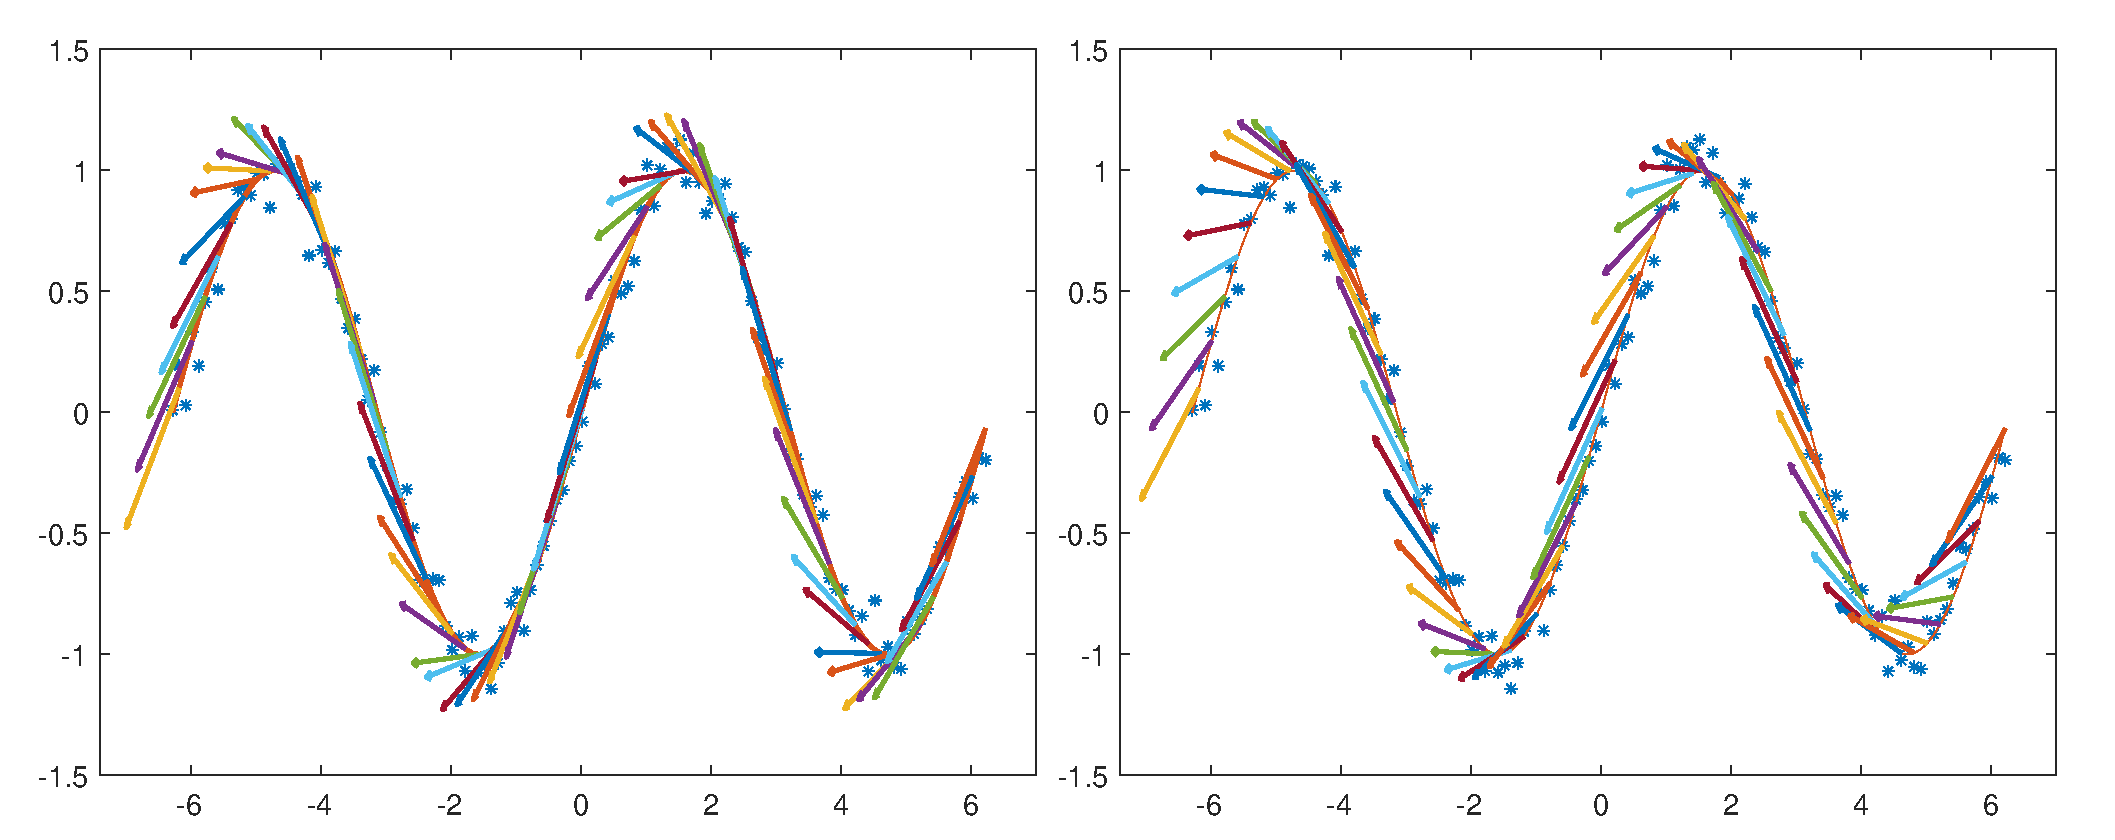
\includegraphics[width=\linewidth]{field_demo.eps} 
   \caption{Illustration of the vector field. Left: using partial nearest samples Right: using all samples}
   \label{fig:example:1}
\end{figure}

The effect of improving the quality of $C(x)$ by neglecting samples with a large scale can be seen in the vector field in Figure \ref{fig:example:1}. The vector field is constructed from the dominant eigenvector of the weighted covariance matrix $C(x)$. In the left diagram, the set $S$ is the $k$-nearest neighborhood of $x$, and in the right diagram the set $S$ represents all the samples. From the figure, we know that by selecting the nearest samples we can get a weighted covariance matrix to approximate the vector field better.

Based on the above intuition, we show that constructing the {\it l}-SCRE by neglecting the far-away samples will help to reduce the point-wise bias of the derivatives. The reduced-bias phenomenon will further lead us to a ridge that is `closer' than that obtained by using all the samples.
 \subsection{Main Contributions}
Our contributions consist mainly of the following:
\begin{itemize}
\item[1.] We propose to use the nearest samples to construct a local version of the SCRE method, and in turn use that to construct the ridge-estimator function. The proposed {\it l}-SCRE  can obtain a ridge that is closer to the original manifold.
\item[2.] We provide the theoretical result of the component-wise bias and variance corresponding to the {\it l}-SCRE and prove that, under mild conditions, the local kernel function can indeed reduce the bias of derivatives more effectively than the KDE-based approaches.
\item[3.] By building the connection Hessian of the estimated density function with the empirical covariance matrix, we show the necessity of rank-one modification to obtain a stable tangent space estimator, which further improves the performance of the {\it l}-SCRE.
%\item[1.] We develop the connection between the two common methods (kernel-density estimation and tangent-space estimation) to define the fitted manifold.
%\item[2.] By analyzing the eigenspace of the Hessian matrix $H(x)$ of the kernel-density estimation function, we show that the normal space is not always generated by the principal eigenvectors of $H(x)$. To solve this problem, we split the $H(x)$ into two parts, $A(x)$ and $B(x)$. By estimating the normal space from $B(x)$, we can get a stable estimate of the normal space. The numerical experiment also demonstrates the effectiveness of our method.
%\item[3.] Our method can not only move an outlier $x_i$ onto the manifold, but also restrict the path of the convergence to be in the normal space of the intended targeting point $c(x)$.
%\item[4.] We also provide a faster algorithm to cope with the vanishing-gradient phenomenon for the kernel-density function.
\end{itemize}
Finally, we provide numerical examples to show the effectiveness of our strategy, and also show that the vector field corresponding to our method is smoother and more appropriate for the manifold-estimation problem.
\subsection{Notations}
The most frequently used symbols and notations are listed in Table 1.%\ref{symbols}.


\begin{table}[h]\label{symbols}
\caption{Symbols and Notations}
\resizebox{14cm}{!}{
\begin{tabular}{c|c}\hline
Symbols & Meaning and Explanation\\\hline
$d$,$D$ & The dimension of the manifold and the dimension of the ambient space\\
${\rm E},{\rm Var}$ & The expectation and the variance operator\\
$\mathcal M,\hat{\mathcal G}$ & The true unknown manifold and the ridge estimator (discrete set)\\ 
$\mathcal M_{\hat{G}}$ & The projection of the ridge estimator $\hat{\mathcal G}$ onto $\mathcal M$\\
$p_n(x),g_n(x),H(x)$& The smooth density function, its gradient, and the Hessian Matrix\\
$\hat{p}_{r,h}(x), g_{\hat{p}_{r,h}}(x),H_{\hat{p}_{r,h}}(x)$& The local KDE estimator, its gradient, and the Hessian Matrix\\
 $\Pi,\Pi^c$ & The projection onto the top $d$ eigenvectors and its orthogonal complement\\
 $f$ & The nonlinear increasing, nonnegative, and concave function\\ 
 $J(x)$ & The semi-positive definite matrix, which is a key component of the Hessian\\  
 {$C(x)$, $H(x)$} &  {The weighted sample covariance matrix and the Hessian matrix at $x$}\\
 $\Pi_H$ & The projection matrix constructed by the top $d$ eigenvectors of $H$ \\ 
 ${\mathcal D}_r(x_0)$ & The $D$-dimensional ball centered at $x_0$ with a radius of $r$\\
 ${\cal N}(x, r)$ & The samples in the neighborhood of $x$ with a radius of $r$ \\
 \hline 
\end{tabular}}
\end{table}


\subsection{Related Work}
\cite{ozertem2011locally} proposed a KDE-based subspace mean-shift algorithm (SCMS) to find the principal curve projection where the kernel density estimator is defined as a data-related covariance sum of kernel functions 
\[
\hat{p}(x) = \frac{1}{n}\sum_i G_{\Sigma_i}(x -x_i).
\] 
{Note that $\hat{p}(x)$ depends only on the $n$.} By setting $\nabla \hat{p}(x) = 0$, we can obtain the mean-shift iteration: 
\[
x\leftarrow m(x) = (\sum_i c_i \Sigma_i^{-1} )^{-1} \sum_i c_i \Sigma_i^{-1}x_i.
\]
Directly applying the mean-shift algorithm will make $x$ converge to the local maximum of $\hat{p}(x)$, which we call a mode. By restricting $x$ to converge to the $d$ dimension ridge defined by $\hat{p}(x)$, the subspace-constrained mean-shift iteration \cite{ozertem2011locally} is given as
\[
x\leftarrow m(x) =V(x)_{\perp} V(x)_{\perp}^T (\sum_i c_i \Sigma_i^{-1} )^{-1} \sum_i c_i \Sigma_i^{-1}x_i,
\]
where $V(x)_{\perp}$ is the eigenvectors corresponding to the $D-d$ largest eigenvectors of the Hessian matrix $\Sigma^{-1} = -\hat{p}^{-1}(x)\hat{H}(x)+\hat{p}^{-2}(x)\hat{g}(x)\hat{g}(x)^T$, where $\hat{H}(x), \hat{g}(x)$ are the Hessian and gradient of $\hat{p}(x)$.

\cite{myhre2016manifold} used the spectral decomposition on the Hessian matrix $H(x) = Q(x)\Lambda(x)Q(x)^T$, and, furthermore, decomposed $Q(x)$ into $Q(x)=[Q_\perp(x), Q_{\|}(x)]$, where $Q_\perp(x)$ is the eigenvectors corresponding to the $d$ largest eigenvalues of $H(x)$. Then, projecting points onto a density ridge can be rendered as the following initial value problem:
\[
\frac{d x(t)}{dt} = Q_{\perp}(x(t)) Q^T_{\perp}(x(t)) g(x(t)), \quad x(0) = x_0,
\]
where $g(x(t))$ is the gradient of $P(x)$ at $x(t)$.

\cite{mohammed2017manifold} also performed the gradient-ascent algorithm in the direction of $V(x)V(x)^Tg(x)$, with $V$ consisting of the eigenvectors corresponding to the $D-d$ largest eigenvalues, and $g(x)$ being the gradient of the approximate squared-distance function (asdf). The asdf is defined as a minus $\log$ transform of density function $p(x)$ or a weighted summation of squared distance for each cylinder.

Besides being defined with a kernel-density function, the manifold can also be defined with the zero points $\{x| F(x)={\bf 0}\}$ of a vector-valued function $F(x): R^D \rightarrow R^D$. Such methods, as used by \cite{fefferman2018fitting, mohammed2017manifold, yao2019manifold}, normally require estimating the local tangent space of the points residing in the neighborhood of the interested point $x$. The vector-valued function $F(x)$ is defined differently in works with different objectives. For example,  \cite{fefferman2018fitting} define the function $F(x)$ as
\[
F(x)= \Pi_x \sum_i \alpha_i(x) \Pi^i(x - x_i).
\]
Furthermore, \cite{yao2019manifold} simplify the two-step projection format into $F(x)= \Pi_x \sum_i \alpha_i(x) (x - x_i)$ by neglecting the inner projection $\Pi^i$. They also show the simplified version, which can also achieve good performance.

The work of \cite{chen2020solution}, albeit tangentially related to the above, provides some theoretical results, such as the smoothness theorem, stability theorem, and convergence property of the gradient flow on the solution manifold. The solution manifold is defined as a set of points satisfying the abstract form $\{x| \Psi(x) = 0\}$.


\section{Manifold Estimation}

We adopt the classical kernel-density estimation approach to handle our manifold-fitting problem, as the majority of previous works do. From the kernel-density perspective, the manifold can be viewed as points that satisfy some specific ridge conditions of the estimated density function.
\subsection{Ridge Definition}
There are two main definitions of a ridge, both of which involve describing the eigenspace of the Hessian and the gradient.
\begin{definition}\label{RR}
A point $x$ is on the $d$-dimensional ridge $R$ of its probability density function when the gradient $g(x)$ is orthogonal to at least $D-d$ eigenvectors of $H(x)$ and the corresponding $D-d$ eigenvalues are negative. See \cite{ozertem2011locally}
\end{definition}
This definition gives us only a condition to test whether a point $x$ lies on the $d$-dimensional ridge. Given any $x$, it does not necessarily tell us how to pull it onto the $d$-dimensional ridge. There are $D-d$ eigenvectors of $H(x)$ that are orthogonal to the gradient $g(x)$, but it does not tell us the eigenvalues of $H(x)$ to which the eigenvectors correspond.

In some other works, such as \cite{genovese2014nonparametric}, the ridge is defined more concretely by restriction of the specific eigenvectors. Given any density function $p(x)$, we can define the ridge as the subset of the domain that satisfies
\begin{equation}\label{ridgeDF}
R = \{x| \Pi^{\perp}(H(x)) g(x) = 0, \lambda_{d+1}(H(x))<0\},
\end{equation}
where $H(x)$ is the Hessian matrix of $p(x)$, $g(x)$ is its gradient, and $\Pi^{\perp}$ is the projection onto the eigenspace spanned by the $D-d$ smallest eigenvalues.

At the sample level, given an empirical density function $\hat{p}(x)$ ($\hat{p}_h(x)$ or $\hat{p}_{r, h}(x)$),  we will have the estimated ridge 
\begin{align*}
\hat{R}_h =&R(\hat{p}_h(x))= \{x| \Pi^{\perp}(H_{\hat{p}_{h}}(x)) g_{\hat{p}_{h}}(x) = 0, \lambda_{d+1}(H_{\hat{p}_{h}}(x))<0\} \quad \mbox{or}\\
\hat{R}_{r, h}=& R(\hat{p}_{r,h}(x))=\{x| \Pi^{\perp}(H_{\hat{p}_{r,h}}(x)) g_{\hat{p}_{r,h}}(x) = 0, \lambda_{d+1}(H_{\hat{p}_{r,h}}(x))<0\},
\end{align*} 
respectively. 

\begin{remark}   
It is worth noting that both the ridge $\hat{R}$ and the estimated ridges, such as $\hat{R}_h$ or $\hat{R}_{r,h}$ are continuous sets.
\end{remark}


When $H(x)$ has exactly $D-d$ negative eigenvalues, these two definitions have no practical differences. However, when $H(x)$ has more than $D-d$ negative eigenvalues, then, from Definition \ref{RR}, we have multiple choices to build the space to satisfy the ridge definition. Under this condition, the ridge in \eqref{ridgeDF} is the only choice, and this ridge, corresponding to definition \eqref{ridgeDF}, is a subset of Definition \ref{RR}.

From the definition, it can be observed that the ridge set $R$ is closely related to the Hessian $H(x)$ and the gradient $g(x)$. The following section will show the connection between the distance between the ridges and the bias of the Hessian and gradient.



\subsection{Ridge Estimation and Error Measurement}
In practice, we use the ridge $R$ as an approximation of the unknown manifold $\mathcal M$ numerically. However, the definition of a ridge in \eqref{ridgeDF} is arguably too descriptive and unrealistic. We can only judge whether a point resides on the ridge, but the definition provides an explicit continuous function to describe the ridge. In reality, starting from a random sample given in advance, we will need an algorithm to push the data points onto the ridge so that the resultant points satisfy the ridge definition. To be specific, what we obtain is a set of modified discrete samples, $\hat{\mathcal G}$, satisfying the ridge definition. To this end, we may further specify the ridge estimator $\hat{\cal G}$ in \eqref{Estimator} by
\[
\hat{\mathcal G} = {\rm Algorithm}(\{x_i, i=1:n\},  \hat{R})
\]
where the estimated $\hat{R}$ can be $\hat{R}_h$ or $\hat{R}_{r,h}$. Note that the resultant $\hat{\mathcal G}$ relies on the initial data points $\{x_i\}$, the estimated ridge $\hat{R}$, and the actual implementation (algorithm) involved in determining how to process the data $\{x_i\}$ by moving them onto the defined ridge. Obviously, we know $\hat{\mathcal G} \subset \hat{R}$.
\begin{figure}[htbp] %  figure placement: here, top, bottom, or page
   \centering
   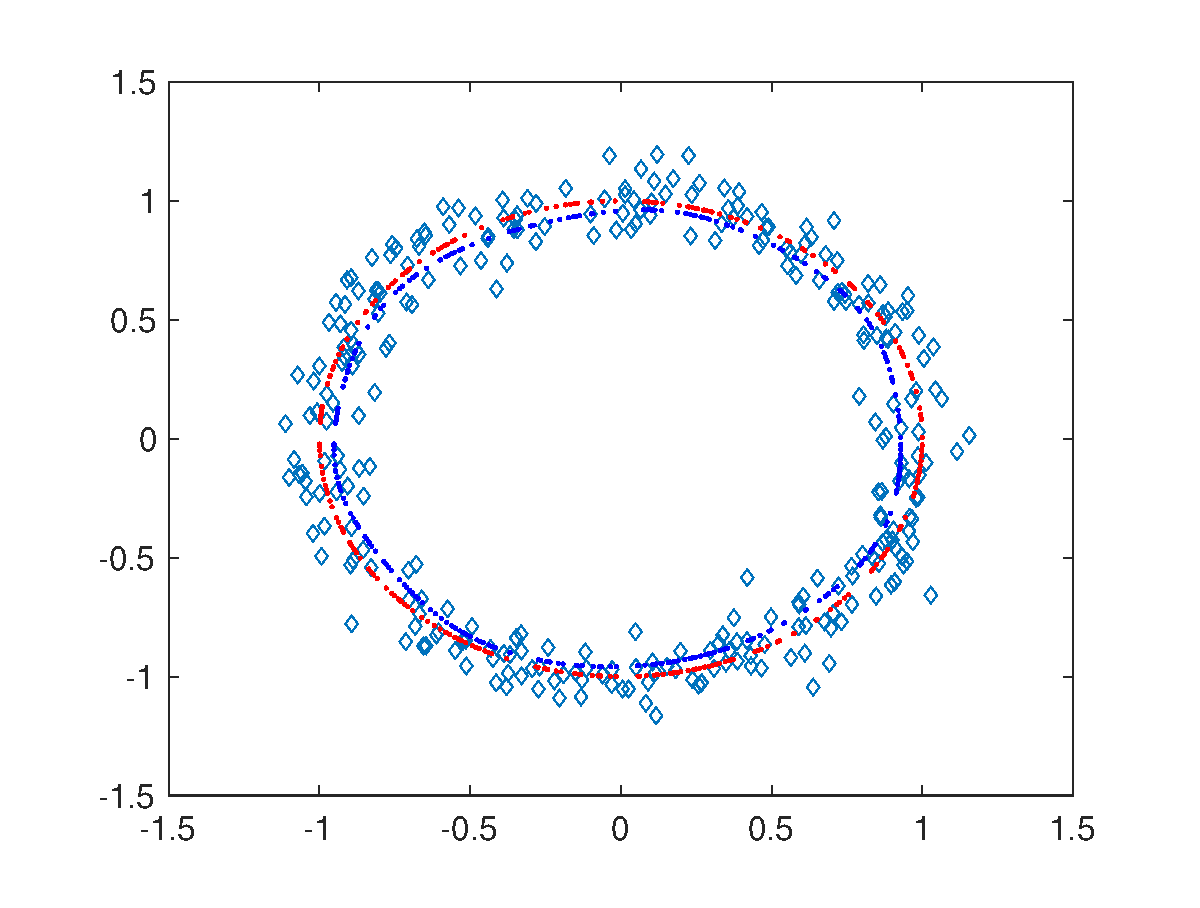
\includegraphics[width=3.5in]{introduction_demo.eps} 
      \caption{Illustration of the $\hat{\mathcal G},\mathcal M, \mathcal M_{\hat{\mathcal G}}$ and the Hausdorff and average margin using the example of a toy circle. The blue diamond markers represent the observation points. The blue dots represent the computed points that satisfy the ridge condition, i.e. $\hat{\mathcal G}$. The red dots represent the projection of $\hat{\mathcal G}$ onto $\mathcal M$, denoted by $\cal M_{\hat{G}}$. }
   \label{fig:example:2}
\end{figure}

Because $\hat{\mathcal G}$ is a discrete set and $\mathcal M$ is supposed to be continuous and smooth, the two sets have different cardinalities. Consider an extreme case where $\hat{\mathcal G}$ is a discrete subset of $\mathcal M$. Clearly, the largest distance from $\mathcal M$ to $\hat{\mathcal G}$ is $\sup_{x\in \mathcal M}\inf_{y\in\hat{\mathcal G}} \|x-y\|_2$, which is largely affected by the distribution of samples in $\hat{\mathcal G}$.

To diminish the random factor in the distance measurement between $\hat{\mathcal G}$ and $\mathcal M$, we extract a subset from $\mathcal M$, ${\mathcal M}_{\hat{\mathcal G}}=\pi_{\mathcal M}(\hat{\mathcal G})$, and consider the Hausdorff distance between ${\hat{\mathcal G}}$ and ${\mathcal M}_{\hat{\mathcal G}}$ (see Figure \ref{fig:example:2}). Since the projection $\pi_{\mathcal M}(\hat{\mathcal G})$ from $\hat{\mathcal G}$ to $\mathcal M_{\hat{G}}$ is onto, the Hausdorff distance equals the quasi-Hausdorff distance
\begin{equation}\label{Hausd}
{\rm Haus}({\hat{\mathcal G}}, {\mathcal M}_{\hat{\mathcal G}}) = \max_{\hat{x}_k\in \hat{\mathcal G}} \min_{\tilde{y}_s\in {\mathcal M}_{\hat{\mathcal G}}}\|\hat{x}_k-\tilde{y}_s\|_2.
\end{equation}
The Hausdorff distance is the largest margin between $\hat{\mathcal G}$ and ${\mathcal M}_{\hat{\mathcal G}}$. The largest margin is dominated by only one point in $\hat{\mathcal G}$, which cannot reflect the overall margin level. So we also consider the average margin, defined as
\begin{equation}\label{margin}
{\rm Marg}({\hat{\mathcal G}, {\mathcal M}_{\hat{\mathcal G}}}) = \frac{1}{|\hat{\mathcal G}|} \sum_{\hat{x}_k\in \hat{\mathcal G}} \min_{\tilde{y}_s\in {\mathcal M}_{\hat{\mathcal G}}}\|\hat{x}_k-\tilde{y}_s\|_2,
\end{equation}
where $|\cal \hat{G}|$ represents the number of samples in $\cal \hat{G}$.
The distances, whether Hausdorff or average margin, are too complicated to bound or optimize directly. Because $\hat{\cal G}\subset \hat{R}$,  we also need to connect $\cal M$ with some ridge under the following assumption:
\begin{assumption}\label{Data_assumption}
Assume there is a density function $p(x)$ such that 
\begin{itemize}
\item[1.] For the ridge $R(p(x))$ derived from $p(x)$: $R(p(x))={\cal M}$.
\item[2.] The projection of $\hat{G}$ onto ${\cal M}$ satisfies ${\cal M}_{\hat{G}}\subset R(p(x))$.
\item[3.] The distance between $R(p(x))$ and $\hat{R}(x)$ is comparable, where $\hat{R}(x)$ is a ridge derived from some empirical functions.
\end{itemize}
% \Yao{Assume the points on $\hat{\cal G}, \cal M_{\hat{G}}$ satisfy the ridge definition corresponding to two density functions $\hat{p}(x), p(x)$ respectively. }
\end{assumption}
\begin{remark}
Since $\cal M$ can also be considered  as a ridge of some density function $p(x)$, the problem of estimating the distance between $\cal M_{\hat{\cal G}}$ and $\hat{\cal G}$ can be converted to one of estimating the distance between two ridges. 
This assumption can be verified by selecting an appropriate form of $p(x)$, for instance by restricting $p(x)$ to nonzero only on $\cal M$. 
\end{remark}
Next, we connect the distance between any pair of ridges $R_1, R_2$ with the analytic quantity (such as gradient and Hessian) of their corresponding density functions $p_1(x), p_2(x)$. 
%We show, for any pair of ridges $R_1$ and $R_2$ (which satisfies the ridge definition of $p_1(x)$ and $p_2(x)$ respectively), 
Specifically, the  distance between $R_1$ and $R_2$ is of the same order as the error of the corresponding derivatives. 
\begin{lemma}{ 
For any $R_1$, $R_2$, and any point $x_1\in R_1$, the pairwise distance from $x_1$ to $R_2$ yields the order of: %$\min_{x_2\in R_2}\|x_1-x_2\|_2$ %between any two ridges $R_1$ and $R_2$ 
%is of order $O(\|H_1(x_1)-H_2(x_1)\|_F+\|g_1(x_1)-g_2(x_1)\|_2)$, 
\[
\min_{x_2\in R_2}\|x_1-x_2\|_2 = O(\|H_1(x_1)-H_2(x_1)\|_F+\|g_1(x_1)-g_2(x_1)\|_2)
\]
where $H_1(x_1), g_1 (x_1)$ are the Hessian and gradient of some estimated density function $p_1(x_1)$ evaluated at $x_1$; $H_2(x_1)$ and $g_2(x_1)$ are the Hessian and gradient of the density function of $p_2(x)$ evaluated at $x_1$, respectively.
%For any two ridges $R, \hat{R}$ defined by $R = \{x| \Pi_{H}(x)g(x) = 0\}$,$\hat{R} = \{x| \Pi_{\hat{H}}(x))\hat{g}(x) = 0\}$, 
 %$d(x, \hat{R}) = O(\|\hat{H}(x)-H(x)\|_F+\|\hat{g}(x)-g(x)\|_2)$
 }\label{margin}
\end{lemma}
The proof of Lemma \ref{margin} can be found in the supplementary material.% appendix \ref{Ridge Derivative Lemma}.
\begin{remark}
Lemma \ref{margin} builds the bridge between the geometric quantities and the analytic differential quantities. Through this lemma, we can easily convert the problem of searching for a `closer' ridge to the problem of searching for a `better' approximation of the Hessian and gradient. As illustrated in Figure \ref{fig:example:3}, this conversion arguably give our work a stronger foundation and greater versatility.
\end{remark}
\begin{figure}[htbp] %  figure placement: here, top, bottom, or page
   \centering
   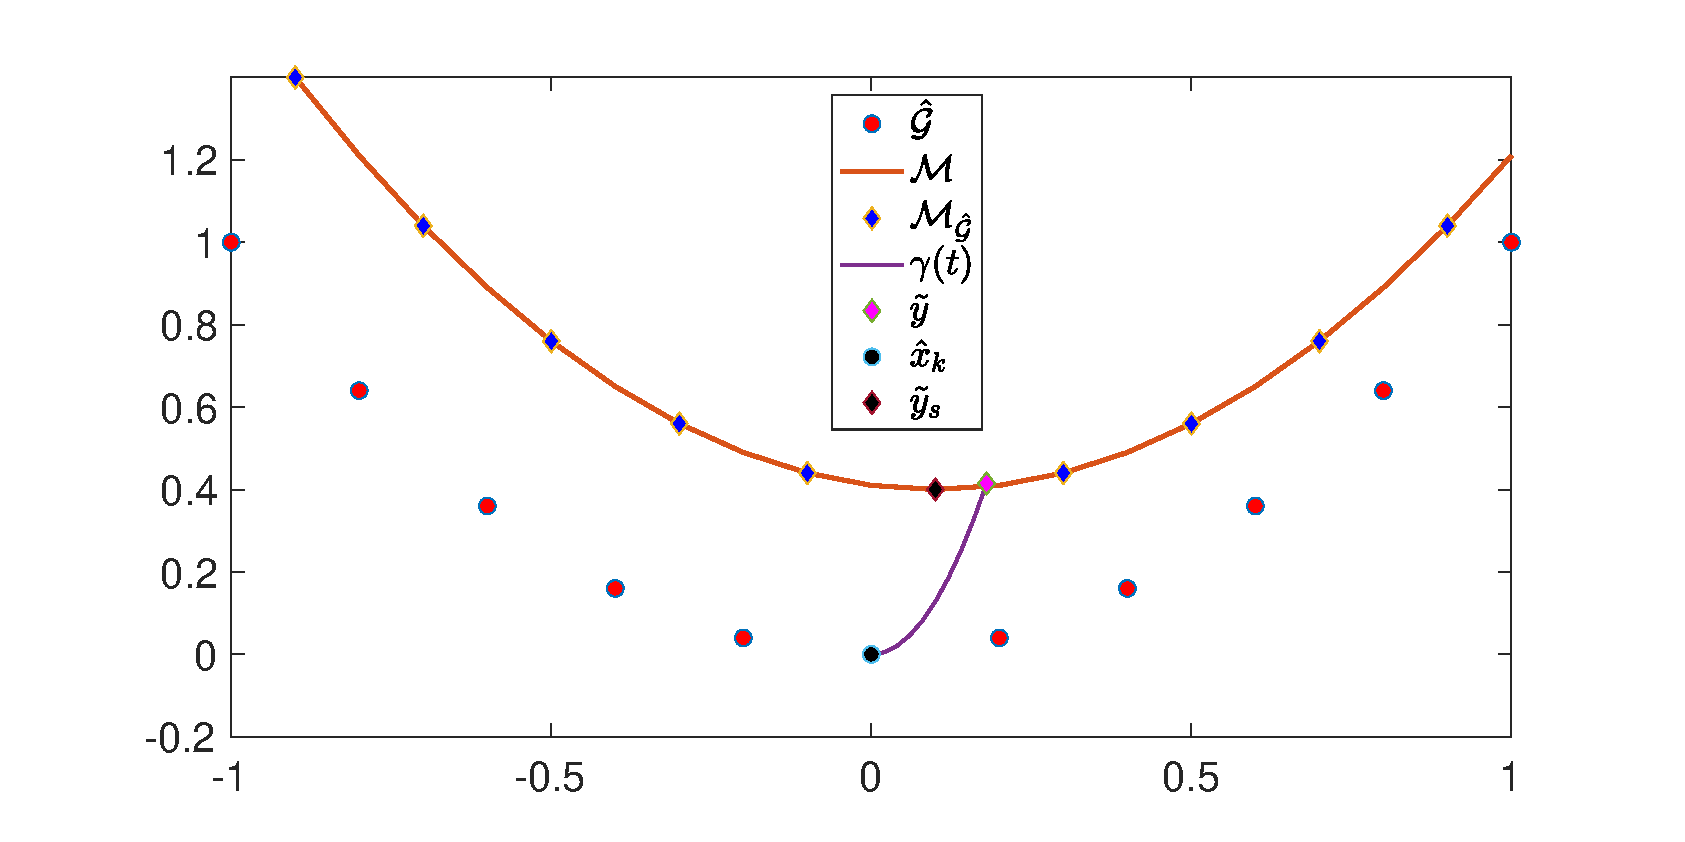
\includegraphics[width=0.8\linewidth]{demoMG.eps} 
   \caption{Illustration of the relationship  between $\hat{\cal G},{\cal M}, {\cal M}_{\cal \hat{G}}, \gamma(t),\hat{x}_k, \tilde{y}, \tilde{y}_s$}
   \label{fig:example:3}
\end{figure}


Using assumption \ref{Data_assumption} and Lemma \ref{margin}, we have, for any $\hat{x}_k\in \hat{\mathcal G}$, a $\tilde{y}\in {\mathcal M}$ that is the end point of the unit speed curve $\gamma(t)$ starting from $\hat{x}_k$. Meanwhile, both  $\hat{x}_k$ and $\tilde{y}$ satisfy the ridge definition in \eqref{ridgeDF}. 
Thus, we know that 
\begin{equation}\label{pointwise-bound}
\min_{\tilde{y}_s\in {\mathcal M}_{\hat{\mathcal G}}}\|\hat{x}_k-\tilde{y}_s\|_2 \leq \|\hat{x}_k-\tilde{y}\|_2 = O (\|H_{\hat{p}}(\hat{x}_k)-H(\hat{x}_k)\|_F+\|g_{\hat{p}}(\hat{x}_k)-g(\hat{x}_k)\|_2  ).
\end{equation}
\begin{remark}
The distance between two discrete sets $\hat{\cal G}, {\cal M}_{\hat{\cal G}}$ is converted to the distance between $\hat{\cal G}$ and ${\cal M}$ by the unit speed curve $\gamma(t)$. $\gamma(t)$ starts from a point in $\hat{\cal G}$ (such as $\hat{x}_k$) with a direction of $\Pi_{H_p}(\gamma(t)) g_{p}(\gamma(t))$. The point at which $\gamma(t)$ goes through $\cal M$ is denoted by $\tilde{y}$. The details of the construction method of the curve $\gamma(t)$ can be found in the supplementary material.
%appendix \ref{Ridge Derivative Lemma}.
\end{remark}
From \eqref{Hausd}, by maximizing the distance with respect to $x_k\in 
\hat{\cal G}$ in \eqref{pointwise-bound}, we know that ${\rm Haus}({\mathcal {\hat{G}}}, {\mathcal M}_{\mathcal {\hat{G}}})$ yields a uniform upper bound by the sup norm at the right side:
\begin{equation}\label{Hausmargin}
{\rm Haus}({\hat{\mathcal G}}, {\mathcal M}_{\hat{\mathcal G}}) = O (\sup_{\hat{x}\in\hat{\cal G}}( \|H_{\hat{p}}(\hat{x})-H(\hat{x})\|_F+\|g_{\hat{p}}(\hat{x})-g(\hat{x})\|_2 ) ),
\end{equation}
where $\hat{p}$ is the estimated density, which can be chosen as $\hat{p}_h(x)$, $\hat{p}_{r,h}(x)$, or any other empirical forms.

\begin{example}
When we approximate $\hat{p}(x), g_{\hat{p}}(x), H_{\hat{p}}(x)$ using the kernel-density function as $\hat{p}_h(x), g_{\hat{p}_h}(x), H_{\hat{p}_h}(x)$, %where the subscript $n$ means the functions are related with the samples and the sample size $n$.
the pairwise error for the derivatives yields the following result:
\[
\begin{aligned}
& ( |g_{\hat{p}_h}(x)-g_p(x)|)_i = O(h^2) + O_p(\sqrt{\frac{1}{{{n h^{D+2}}}}}),\\
& ( |H_{\hat{p}_h}(x)-H_p(x)| )_{ij} = O(h^2) + O_p(\sqrt{\frac{1}{{{n h^{D+4}}}}}).
\end{aligned}
\]
The empirical-process theory gives the uniform error as
\[
\begin{aligned}
& \sup_x( |g_{\hat{p}_h}(x)-g_p(x)|)_i = O(h^2) + O_p(\sqrt{\frac{\log n}{{{n h^{D+2}}}}}),\\
& \sup_x( |H_{\hat{p}_h}(x)-H_p(x)| )_{ij} = O(h^2) + O_p(\sqrt{\frac{\log n}{{{n h^{D+4}}}}}).
\end{aligned}
\]
The error rates for the pairwise and uniform differ only in the stochastic term, with a scale of $\sqrt{\log n}$. See \cite{chen2017tutorial,JMLR:v17:ariascastro16a, genovese2014nonparametric}.
\end{example}
%From \eqref{Hausmargin}, we can conclude that the Hausdorff distance of ${\mathcal G}$ and ${\mathcal M}_{\mathcal G}$ is controlled by the uniform approximation error of the Hessian and gradient, as $\sup_x( \|H_n(x)-H(x)\|_2+\|g_n(x)-g(x)\|_2$. The uniform derivatives rate is proved to be $L_{\infty}$, and the norm as , where the difference is the result of introducing $\log n$. This result is shown in \cite{JMLR:v17:ariascastro16a, genovese2014nonparametric}.
%Clearly, the Hausdorff distance between is the largest gap. As shown in \cite{genovese2014nonparametric}, the Hausdorff distance between the manifold and the ridge yields a uniform bound 
%${\rm Haus}({\mathcal G}, {\mathcal M}_{\mathcal G}) = O(h^2) + O_p((\frac{\log n}{{{n h^{d+4}}}})^{1/2})$. When $h={(\frac{\log n}{n}})^{1/(d+8)}$, the optimal minimum achieved is $O_p((\frac{\log n}{n})^{2/(d+8)})$. This optimum is the estimated convergent speed for the Hausdorff distance with the process of increasing the sample size $n$ and simultaneously decreasing $h$. However, in this paper, we mainly focus on how to get a closer ridge under the current observations, i.e. the number of samples is fixed.

Unlike the upper bound of the Hausdorff distance shown in \eqref{Hausmargin}, the average margin ${\rm Margin}(\hat {\mathcal G}, M_{\hat{\cal G}})$ is closely related to the point-wise approximation error of $O (\|H_{\hat{p}_h}(x)-H_p(x)\|_F+\|g_{\hat{p}_h}(x)-g_p(x)\|_2)$. To reduce the average margin, we should focus on finding a new density function to improve the point-wise error with respect to the gradient and Hessian, and hope that this improvement of the error will lead to good performance of the estimated ridge.

To our knowledge, the most widely used nonparametric approach to approximate $p(x)$ is the KDE method. Therefore, we will review the classical KDE approach to approximate a density function, and derive the details of the corresponding derivatives' approximation error.
\subsection{Derivatives for KDE}
%Suppose we have multidimensional samples $\{x_k, x_k \in {\mathbb R}^D\}$ from a distribution $p(x)$. Then, we can build a kernel density function to estimate $p(x)$ using the kernel's summation from all the samples, as follows:
%\begin{equation}\label{KDE}
%p_n(x) = \frac{1}{n h^D} \sum_k K(\frac{x-x_k}{h}).
%\end{equation}
%The kernel $K(u)$ is supposed to be positive and differentiable at least with an order 2 and satisfies
%\[
%\int K(u) du = 1, \int u K(u) du = 0, \int \|u\|_2^2 K(u) du >0.
%\]
The derivatives' bias generated from the kernel-density function is highly related to the distance between the ridges constructed by $p(x)$ and $\hat{p}_h(x)$, respectively. We introduce the bias of the first-order and second-order derivatives when using the kernel-density function to approximate the real density function.
\subsubsection{Derivative Bias}
To derive the bias of the first-order and second-order derivatives, we need to repeatedly implement the integration by the substitution method on the multiple-variable function. For the sake of completeness, we first recall some results for the bias and variance with respect to the derivatives. Subsequently, we show that using $\hat{p}_{r,h}(x)$ can improve the bias and variance results more than using $\hat{p}_{h}(x)$.

\begin{theorem}
The bias of the first order and second order of the $\hat{p}_h(x)$ is 
\begin{equation*}\label{BiasResult}
|{\rm E}(\partial_{x_s}  \hat{p}_h(x)) - \partial_{x_s}p(x)|  = \frac{h^2|\Delta (\partial_{x_s}p(x))|}{2D}  \int \|u\|_2^2 K(u) du+o(h^2),
\end{equation*}
\begin{equation*}\label{order2}
|{\rm E}( \partial_{x_s} \partial_{x_t}  \hat{p}_h(x)) -  \partial_{x_s} \partial_{x_t} p(x)| = \frac{h^2 |\Delta (\partial_{x_s}\partial_{x_t} p(x))|}{2D} \int \|u\|_2^2 K(u) du+o(h^2).
\end{equation*}
where $\Delta$ is the Laplace-Beltrami operator.
\end{theorem}
The details of the procedure for proof can be found in the supplementary material.%appendix \ref{bias_proof}.

\remark{
The Laplace-Beltrami operator is the divergence of the gradient. For any $f(x)$, $\Delta f(x)$ is the summation of the diagonal elements of $H_f(x)$ (the Hessian of $f(x)$), which is also the summation of the eigenvalues of $H_f(x)$.
}
% The largest eigenvalue of the Hessian matrix $H(\partial_{x_s}p(x))$ and $\Delta (\partial_{x_s}\partial_{x_t}p(x))$ is the largest eigenvalue of the matrix $M_{st}$, whose $i,j$-th element is $\frac{\partial^4}{\partial x_s\partial x_t \partial x_i \partial x_j} p(x)$, i.e. $\lambda_{st}(x)= \max_k \lambda_k( M_{st}(x))$.

\begin{remark}
It should be noted that in \eqref{BiasResult} the square term $h^2$ originates from the fact that the positive kernel is of order 2, which is fixed and cannot be improved. However, we can make $\int \|u\|_2^2 K(u)du$ much smaller by making a small modification-{\it truncating the kernel}-as discussed below.
\end{remark}
\subsubsection{Derivative Variance}
After we get the bias of the derivatives, in order to gain a better understanding of the stochastic property of the derivatives, we should also consider the variance. In this section, we give the variance result of the first and second derivatives of the KDE under the i.i.d. samples assumption. 

Let $\phi_s(x)$ and $\phi_{s,t}(x)$ be
\[
\phi_s(x) = p(x) \int (\partial_{ u_s } K (u) )^2 du,\quad  \phi_{s,t}(x) = p(x) \int (\partial_{u_s}\partial_{u_t} K (u) )^2 du
\]
\begin{theorem}
The variance of the first- and second-order derivatives for $\hat{p}_h(x)$ has the following bound: 
\begin{equation*}\label{VarResult}
\begin{aligned}
&{\rm E} |\partial_{x_s} \hat{p}_h(x)-{\rm E}(\partial_{x_s} \hat{p}_h(x))| = \sqrt{\frac{\phi_s(x)}{n h^{D+2}}}+O(\frac{1}{n^{1/2}h^{(D+1)/2}}),\\
&{\rm E} | \partial_{x_s}\partial_{x_t} \hat{p}_h(x) -{\rm E}(\partial_{x_s}\partial_{x_t} \hat{p}_h(x))| = \sqrt{\frac{\phi_{s,t}(x)}{nh^{D+4}}}+O(\frac{1}{n^{1/2}h^{(D+3)/2}}).
\end{aligned}
\end{equation*}
%where $M(u) = \partial_{u_s}K(u)$ and $N(u) = \partial_{u_t}\partial_{u_s}K(u)$, respectively.
\end{theorem}
The details of the procedure for proof can be found in the supplementary material. %appendix \ref{variance_proof}.

\subsubsection{Optimal-Parameter Dilemma}
The bandwidth parameter $h$ controls the smoothness of the density function and its derivatives. We can derive the best possible $h$ to obtain the best approximation error for the kernel-density function. However, we cannot select a single optimum $h$ to be the optimum solution for the multiple objectives, such as the first-order and second-order derivatives.

Using the triangle inequality of absolute function, we derive the upper bound for  $|\partial_{x_s} \hat{p}_h(x) - \partial_{x_s} p(x)|$ by
\[
|\partial_{x_s} \hat{p}_h(x) - \partial_{x_s} p(x)|\leq |{\rm E}(\partial_{x_s}  \hat{p}_h(x)) - \partial_{x_s}p(x)|+ |{\rm E}  (\partial_{x_s} \hat{p}_h(x)) -\partial_{x_s}\hat{p}_h(x)| .
\]
The first term $|{\rm E}(\partial_{x_s}  \hat{p}_h(x)) - \partial_{x_s}p(x)|$ is deterministic and the second term $|{\rm E}  (\partial_{x_s} \hat{p}_h(x)) -\partial_{x_s}\hat{p}_h(x)|$ is a random variable. From \eqref{BiasResult} and \eqref{VarResult}, we know the upper bound of $|\partial_{x_s} \hat{p}_h(x) - \partial_{x_s} p(x)| $ is
\[
|\partial_{x_s} \hat{p}_h(x) - \partial_{x_s} p(x)| =  \frac{h^2|\Delta (\partial_{x_s}p(x))|}{2D}  \int \|u\|_2^2 K(u) du +O_p( \sqrt{\frac{\phi_s(x)}{n h^{D+2}} } ).
\]
Clearly, for the first-order partial derivative, the optimum $h$ should minimize the objective $C_1(x)h^2+C_2(x)\frac{1}{\sqrt{n h^{D+2}}}$. Thus, $h = O({n^{-\frac{1}{D+6}}})$.
\[
|\partial_{x_s}\partial_{x_t} \hat{p}_h(x) - \partial_{x_s}\partial_{x_t} p(x)| = \frac{h^2 |\Delta (\partial_{x_s}\partial_{x_t} p(x))|}{2D} \int \|u\|_2^2 K(u) du + O_p(\sqrt{\frac{\phi_{s,t}(x)}{nh^{D+4}}}).
\]
In the same way, for the second-order partial derivative, the optimum $h$ should minimize the objective $C_3(x)h^2+C_4(x)\frac{1}{\sqrt{n h^{D+4}}}$ as well. Thus, $h = O(n^{-\frac{1}{D+8}})$. Clearly, we cannot minimize the first and second derivative approximations at the same time.

Next, we bring in another parameter, $r$, to restrict our objective function such that we can construct the {\it l}-SCRE by using only the samples with better quality in a surrounding neighborhood of $x$.
%\section{Locally Defined Kernel-Density Estimation}
\section{{\it l}-SCRE}
In this section, we propose the estimator derived from a local kernel-density function, which is called {\it l}-SCRE.
We consider a type of generalized, locally defined kernel, $K_r (\frac{x-x_i}{h})$, controlled by two parameters $r$ and $h$, $h$ being the bandwidth that controls the distribution of each of the samples $x_i$ in a soft manner, and $r$ determining which partition of the samples should be used in our kernel-density function.
\begin{equation}\label{GKDE}
\hat{p}_{r, h}(x) = \frac{1}{n h^D}\sum_i K(\frac{x-x_i}{h}) I(\|x -x_i\|_2\leq r),
\end{equation}
where $I(\cdot)$ is the indicator function, which equals 1 when the condition is met, and 0 otherwise.
The necessity of bringing in the kernel with two parameters is a result of the fact that, in some cases, we will fall into the dilemma of having to use a large $h$ to get a smoother estimation, while, at the same time, needing a smaller $h$ to keep a low bias for the estimated density function and even the derivatives.

It should be noted that in \eqref{GKDE} we consider only the samples in the ball with a radius of $r$; this can also be regarded as a truncated kernel function using the following definition:
\begin{equation}\label{TK}
K_r(\frac{x-x_i}{h}) = K(\frac{x-x_i}{h}) I(\|x -x_i\|_2\leq r).
\end{equation}
Note that $K_r(\frac{x-x_i}{h})$ is not differentiable where $\|x-x_i\|_2=r$. From \eqref{TK}, we also know that for $x$ such that $\|x-x_i\|< r$,
\begin{equation}\label{DTK}
|\frac{\partial}{\partial x_s} K_r(\frac{x-x_i}{h}) | \leq |\frac{\partial}{\partial x_s} K(\frac{x-x_i}{h})|.
\end{equation}
Clearly, $K(u)$ satisfies $\int K(u)du=1$. When necessary, we can also renormalize $K_r(u)$ by a constant value $c>1$, such that
\[
\int c K_r (u) du =  c\int_{\|u\|\leq r/h} K(u) du= 1.
\]
When selecting $K(u)$ as the exponential decreasing function $K(u) = \frac{1}{{(2\pi)}^{d/2}}\exp(-\frac{1}{2}\|u\|^2_2)$, the error for a non-normalized $K_r(u)$ will be small. Using the Gaussian integral formula, we know 
\begin{equation}\label{Perror}
 \int_{\|u\|\leq r/h} K(u) du =1- O(\exp(-(r^2/h^2))).
\end{equation}
When $r$ is larger than $h$, the residue part $O(\exp(-(r^2/h^2)))$ will become ignorable. %We use this relation in the subsequent bias-analysis section.
\subsection{Parameter Setup}
Suppose the true density function $p(x)$ is a constant on $\cal M$ and the observations $\{x_i\}$ are evenly sampled from $p(x)$. However, the shape of the manifold $\cal M$ can be very complicated, for instance a twisted two-dimensional surface embedded in the three-dimensional ambient space. In this case, the kernel-density estimated function $\hat{p}_h(x)$ will have the following characteristics:
\begin{itemize}
\item[1.] If the manifold in the neighborhood of ${\mathcal D}_r(x)$ is complicated, $\hat{p}_h(x)$ will be large because the neighborhood of $x$ will contain more observations.
\item[2.] If the manifold in the neighborhood of ${\mathcal D}_r(x)$ is relatively simple, for instance a flat surface, $\hat{p}_h(x)$ will be small because the neighborhood of $x$ will contain far fewer observations.
\end{itemize}
Recall that $n$ is the total number of observations. The expected number of observations in ${\mathcal N}(x_0 ,r)$ is 
\[
{\rm E}(\sum_i I(x_i\in {\mathcal N}(x_0 ,r)))=n \int_{u\in {\cal M}\cap{\mathcal D}_r(x_0) } p(u) du.
\]

Based on the above analysis, we know that a larger value of $\hat{p}(x)$ implies a complicated structure of $\cal M$ in the neighborhood of $x$, and a smaller value of $\hat{p}(x)$ implies a simple structure of $\cal M$ in the neighborhood of $x$.
For the complicated area of ${\cal D}_r(x) \cap\cal M$, we should focus on an area ${\cal D}_r(x)$ with a small radius $r$. For the simple area of ${\cal D}_r(x) \cap\cal M$, we can enlarge $r$, which could speed up our fitting process.
%
%For a density function defined on a manifold $\mathcal M$ that is embedded in $\mathbb{R}^d$, if the density function $p(x)$ is large at $x_0$, we assume the manifold is more complicated at $x_0$ as it has a smaller local reach. In such a case, we would prefer to construct our local kernel-density function in a smaller neighbor ${\mathcal N}(x_0,r)$. Conversely, if the density $p(x)$ is small, to obtain a more accurate estimation from the data, we would prefer to concentrate on a relatively large area.
%
%For a particular $x$ such that $p(x)$ is relatively large, there is a high probability of sample $x_i$ being generated around $x$, i.e. the sample density around $x$ is higher relative to other places.
%In this paper, we assume that the parameter $r$ is related to the current $x$, from the intuition that when $p(x)$ is large a small partition

In this way, we can select $r$ adaptively and think of it as a function of the true density function $p(x)$; this is denoted by $r(x)$. We determine $r(x)$ by requiring the accumulating density function 
\[
\phi(x,r) = \int_{y\in {\cal M}\cap {\mathcal D}_r(x)} p(y) dy,
\] 
to be a constant $\theta$. %such that the following value $\phi(x,r) $ is a constant $C$. $\phi(x,r)$ is defined as
The implicit function $\phi(x,r)=\theta$ can determine the function $r(x)$.
Note that we can approximate the accumulating density function $\phi(x,r)$ with the samples:
\[
\phi(x,r) \approx \frac{1}{n} \sum_k I(x_k\in {\mathcal N}(x,r)).
\]
In real computational cases, $r(x)$ can be chosen adaptively as the smallest radius that still fulfils the condition that the set $\{x_i | \|x-x_i\|\leq r\}$ contain exactly $m$ elements, where $m$ is a predefined parameter.
%\subsection{Bias and Variance of Derivative of  $p_{r,h}(x)$}

As with the bias for the derivative of $\hat{p}_h(x)$, we also have the bias for the derivative $\hat{p}_{r,h}(x)$. It is easy to show that, under some mild conditions, the bias of the derivatives of $\hat{p}_{r,h}(x)$ is smaller than that of $\hat{p}_h(x)$.
\subsection{Upper Bound of the Bias}
In the previous section, we derived the upper bound of the bias for the classical $\hat{p}_h(x)$. Here, we present the bias result of $\hat{p}_{r,h}(x)$, and show that, under some mild conditions, the bias of the derivatives $\hat{p}_{r,h}(x)$ is smaller than that of $\hat{p}_h(x)$.
%\[
%|{\rm E}(\partial_{x_s}  p_n(x)) - \partial_{x_s}p(x)|  \leq \frac{\lambda_s(x)}{2} h^2 \int \|u\|^2 K(u) du+o(h^2)
%\]

Given any parameter $r,h$ and a density function $p(x)$, we can define two functions $B_s(x| r,h, p)$ and $B_{s,t}(x| r,h, p)$ as
\[
B_s(x| r,h, p)  = \frac{h^2|\Delta (\partial_{x_s}p(x))|}{2D} \int_{\|u\|\leq r /h} \|u\|_2^2 K(u) du
+ |\partial_{x_s} p(x)| \int_{\|u\|\geq r/h} K(u) du
\]
\begin{multline*}
B_{s,t}(x|r,h, p) = \frac{h^2|\Delta (\partial_{x_s}\partial_{x_t} p(x))|}{2D}  \int_{\|u\|\leq r /h} \|u\|_2^2 K(u) du
 + |\partial_{x_s} \partial_{x_t} p(x)| \int_{\|u\|\geq r/h} K(u) du
\end{multline*}
\remark{
From the definition of $B_s(x| r,h, p)$ and $B_{s,t}(x|r,h, p)$, 
if $\|u\|_2>1$, %decreases slower than ${1}/{\|u\|_2^2}$, 
the first term will become a major part because of the existence of the term $\int_{\|u\|\leq r /h} \|u\|_2^2 K(u) du$. 
Taking the limit for $r\rightarrow+\infty$, we will of course have
\begin{equation}\label{asy}
\lim_{\|r\|\rightarrow+\infty} B_s(x|r,h,p) =  \frac{h^2|\Delta (\partial_{x_s}p(x))|}{2D} \int \|u\|_2^2 K(u) du,
\end{equation}
where the right side is the bias of the first derivative for $\hat{p}_{h}(x)$.
}
\begin{lemma} \label{lSCRE}For the derivatives of $\hat{p}_{r,h}(x)$, we have the bias relationship for first- and second-order derivatives as
\begin{gather*}\label{order11}
|{\rm E}( \partial_{x_s}  \hat{p}_{r,h}(x)) -  \partial_{x_s } p(x)|  \leq B_s(x| r,h, p)  ,\\
|{\rm E} (\partial_{x_s} \partial_{x_t}   \hat{p}_{r, h}(x)) -  \partial_{x_s} \partial_{x_t} p(x)| \leq B_{s,t}(x| r,h, p).
\end{gather*}
Furthermore, if  
\begin{equation}\label{condition1}
r \geq\max \{ h, \sqrt{\frac{2|\partial_{x_s} p(x)|}{ |\Delta(\partial_{x_s} p(x))|}} , \sqrt{\frac{2|\partial_{x_s} \partial_{x_t} p(x)|}{ |\Delta(\partial_{x_s}\partial_{x_t} p(x))|}}\},
\end{equation}
the bound of the pairwise derivatives' bias for $\hat{p}_{r,h}(x)$ %{\it l}-SCRE 
will be bounded by that of $\hat{p}_h(x)$%SCRE. In other words,
\begin{gather}\label{bias_bound2}
|{\rm E}( \partial_{x_s}  \hat{p}_{r,h}(x)) -  \partial_{x_s } p(x)| \leq |{\rm E}( \partial_{x_s}  \hat{p}_{h}(x)) -  \partial_{x_s } p(x)|,\\
|{\rm E}( \partial_{x_s} \partial_{x_t} \hat{p}_{r,h}(x)) - \partial_{x_s} \partial_{x_t} p(x)| \leq |{\rm E}( \partial_{x_s}  \partial_{x_t} \hat{p}_{h}(x)) -  \partial_{x_s }\partial_{x_t} p(x)|.\label{bias_bound3}
\end{gather}
\end{lemma}
The proof can be found in the supplementary material.
\remark{
To obtain \eqref{bias_bound2} and \eqref{bias_bound3}, we show that, under the conditions of \eqref{condition1}, the upper bounds $B_s(x| r,h, p)$ and $B_{s,t}(x| r,h, p)$ are less than the pairwise biases $|{\rm E}( \partial_{x_s}  \hat{p}_{h}(x)) -  \partial_{x_s } p(x)|$ and $|{\rm E}( \partial_{x_s}  \partial_{x_t} \hat{p}_{h}(x)) -  \partial_{x_s }\partial_{x_t} p(x)|$, respectively. Thus, we have
\begin{equation}\label{bound-inequality}
|{\rm E}( \partial_{x_s}  \hat{p}_{r,h}(x)) -  \partial_{x_s } p(x)| \leq B_s(x| r,h, p) \leq |{\rm E}( \partial_{x_s}  \hat{p}_{h}(x)) -  \partial_{x_s } p(x)|
\end{equation}
The procedure for obtaining the result for $|{\rm E}( \partial_{x_s} \partial_{x_t} \hat{p}_{r,h}(x)) - \partial_{x_s} \partial_{x_t} p(x)|$ is similar.
}

\subsection{Ridge-Improvement Justification}
%By bringing in two parameters $\gamma,\mu_s(x)$ Lemma \ref{LKDE bias} can be further simplified as Lemma \ref{bias_theorem}.
We are interested in the ratio of the bias improvement. From \eqref{bound-inequality}, we have
\[
\frac{|{\rm E}( \partial_{x_s}  \hat{p}_{r,h}(x)) -  \partial_{x_s } p(x)|}{|{\rm E}( \partial_{x_s}  \hat{p}_{h}(x)) -  \partial_{x_s } p(x)|} \leq \frac{B_s(x| r,h, p)}{|{\rm E}( \partial_{x_s}  \hat{p}_{h}(x)) -  \partial_{x_s } p(x)|}
\]
For notational convenience, we bring in three notations, $\gamma, \mu_s(x,r,h), \mu_{s,t}(x,r,h)$, to simplify the result in Lemma \ref{lSCRE}.
%\[
%\begin{aligned}
%&\gamma = \frac{\int_{\|u\|\geq r/h } \|u\|_2^2 K(u) du}{ 2\int_{\|u\|\geq r/h} K(u) du },\\
%&\mu_s(x,r,h) = \frac{\Delta (\partial_{x_s}p(x)) h^2 \int_{\|u\|\leq r /h} \|u\|_2^2 K(u) du +  2\int_{\|u\|\geq r/h} K(u) du |\partial_{x_s} p(x)|}{\Delta (\partial_{x_s}p(x)) h^2 \int\|u\|_2^2 K(u) du },\\
%&\mu_{s,t}(x,r,h) = \frac{\Delta (\partial_{x_s}\partial_{x_t} p(x)) h^2 \int_{\|u\|\leq r /h} \|u\|_2^2 K(u) du +  2\int_{\|u\|\geq r/h} K(u) du |\partial_{x_s} \partial_{x_t}p(x)|}{\Delta (\partial_{x_s}\partial_{x_t} p(x)) h^2 \int\|u\|_2^2 K(u) du }.
%\end{aligned}
%\]
\begin{gather*}
\gamma(r,h) = \frac{\int_{\|u\|\geq r/h } \|u\|_2^2 K(u) du}{ 2\int_{\|u\|\geq r/h} K(u) du }, \quad
\mu_s(x,r,h) = \frac{B_s(x| r,h, p)}{|{\rm E}( \partial_{x_s}  \hat{p}_{h}(x)) -  \partial_{x_s } p(x)|},\\
\mu_{s,t}(x,r,h) = \frac{B_{s,t}(x| r,h, p)}{|{\rm E}( \partial_{x_s}\partial_{x_t}  \hat{p}_{h}(x)) -  \partial_{x_s } \partial_{x_t}p(x)|}
\end{gather*}

\remark{
Clearly, there exists $r_0 = h$ such that, when $r > r_0$($\|u\|_2>1$), we have $\|u\|_2^2K(u)\geq K(u)$, which implies $\gamma(r_0,h)\geq 1/2$.
%When $r/h \geq 1$, we have, for $\|u\|_2>r/h$, $\|u\|_2^2K(u)\geq K(u)$, which implies $\gamma\geq 1/2$.  
}
\remark{ The observation that $K(u)$'s value approaches 0 as $\|u\|_2$ increases is important for our choice of $r$. Because of \eqref{asy}, we have the following:
\[
\lim_{r \rightarrow \infty }\mu_s(x,r,h) =1,  \lim_{r \rightarrow \infty }\mu_{s,t}(x,r,h) =1.
\]
The scalars $\mu_s(x,r,h)$ and $\mu_{s,t}(x,r,h)$ decrease as $r$ increases. Thus, we need to choose a relatively smaller $r_0$ to ensure that {\it l}-SCRE is more effective than SCRE.
}
\remark{
For any $x\in {\mathbbm R}^D$, there is $r_0(x,h,s)$ (depending on $x$, $h$, and $s$), such that, when $r >r_0(x,h,s)$, the following inequality holds: 
%\[
%\begin{aligned}
%&2\int_{\|u\|\geq r/h} K(u) du |\partial_{x_s} p(x)| < \lambda_{s}(x) h^2 \int_{\|u\|\geq r/h}\|u\|_2^2 K(u) du, \\
%&2\int_{\|u\|\geq r/h} K(u) du |\partial_{x_s}\partial_{x_t} p(x)| < \lambda_{s,t}(x) h^2 \int_{\|u\|\geq r/h}\|u\|_2^2 K(u) du.
%\end{aligned}
%\]
\[
2 D|\partial_{x_s} p(x)|\int_{\|u\|\geq r/h} K(u) du <|\Delta (\partial_{x_s}p(x))| h^2 \int_{\|u\|\geq r/h}\|u\|_2^2 K(u) du,
\]
Similarly, for any $x\in {\mathbbm R}^D$, there is $r_0(x,h,s,t)$ (depending on $x$, $h$, $s$, $t$), such that, when $r >r_0(x,h,s,t)$, the following inequality holds:
\[
2 D |\partial_{x_s}\partial_{x_t} p(x)| \int_{\|u\|\geq r/h} K(u) du < |\Delta (\partial_{x_s}\partial_{x_t}p(x))| h^2 \int_{\|u\|\geq r/h}\|u\|_2^2 K(u) du
\]
}
Using the above two inequalities and the form of $\mu_s(x,r,h),\mu_{s,t}(x,r,h)$, we know that
\[
r_0(x,h) = \max \{ \max_{s}r_0(x,h,s), \max_{s,t}r_0(x,h,s,t)\},
\]
such that, when $r\geq r_0(x,h)$, for any $s,t$, we have
\[
0<\mu_s(x,r,h)<1,\quad 0<\mu_{s,t}(x,r,h)<1.
\]
Substituting $\mu_s(x,r,h), \mu_{s,t}(x,r,h)$ into the results in Lemma \ref{lSCRE} will naturally lead to Lemma \ref{bias_theorem}.

%As a result, we can provide a sufficient condition under which it is better to use the LKDE instead of the KDE for the bias reduction.


\begin{lemma}\label{bias_theorem}
For any $x\in {\mathbbm R}^D$, there is $r_0(x,h)$ (depending on $x$, $h$), such that, when $r> r_0(x,h)$, for any $s, t$, the following two inequalities hold:
%If $|\partial_{x_s} p(x)| \leq \gamma h^2 \lambda_s(x)$ and $|\partial_{x_s} \partial_{x_t} p(x)| \leq \gamma h^2 \lambda_{s,t}(x)$, there is $0<\mu_s(x)<1,0<\mu_{s,t}(x)<1$ such that the bias of $\partial_ {x_s} \hat{p}_{r,h}(x)$ and $\partial_{x_s} \partial_{x_t}  \hat{p}_{r, h}(x)$ will satisfy both of the following inequalities:
\begin{gather*}
|{\rm E} (\partial_ {x_s} \hat{p}_{r,h}(x)) -\partial_{x_s} p(x)| \leq  \frac{ \mu_s(x,r,h)h^2 |\Delta (\partial_{x_s}p(x))|}{2D} \int \|u\|_2^2 K(u) du,\\
|{\rm E} (\partial_{x_s} \partial_{x_t}  \hat{p}_{r, h}(x))-  \partial_{x_s} \partial_{x_t} p(x)| \leq   \frac{\mu_{s,t}(x,r,h)h^2|\Delta (\partial_{x_s}\partial_{x_t}p(x))|}{2D}  \int \|u\|_2^2 K(u) du,
\end{gather*}
where the parameters are $\mu_s(x,r,h)\in(0,1), \mu_{s,t}(x,r,h)\in(0,1)$.
\end{lemma}
%The proof of Theorem \ref{bias_theorem} can be found in Appendix \ref{Simplified Bias Result}.
\begin{remark}
From comparing the above results with \eqref{BiasResult} and \eqref{order2}, we can conclude that the bias for the derivatives of $\hat{p}_{r,h}(x)$ is reduced with a scale of $\mu_s(x,r,h)\in(0,1)$ and $\mu_{s,t}(x,r,h)\in(0,1)$. In the following subsection, we determine that the derivative's variance of $\hat{p}_{r,h}(x)$ is also bounded by that of $\hat{p}_h(x)$.
\end{remark}

\subsubsection{Variance of Upper Bound}
Recall that the variance of the partial derivative is
\[
{{\rm Var}}(\partial_{x_s} \hat{p}_h(x)) = \frac{1}{n h^{D+2}}  (p(x) \int (\partial_{ u_s } K (u) )^2  du + O(h)).
\] 
Here, we can show that the variance of the derivative of $\hat{p}_{r,h}(x)$ also has a similar upper bound to that of $\hat{p}_{h}(x)$.
\begin{theorem}{The variance of derivative of $\hat{p}_{r,h}(x)$ is controlled by}
\[
{{\rm Var}}(\partial_{x_s} \hat{p}_{r,h}(x)) \leq \frac{1}{n h^{D+2}}  (p(x) \int (\partial_{ u_s } K (u) )^2   du + O(h)).
\]
\end{theorem}
The proof can be found in the supplementary material.  %appendix \ref{Derivatives' Variance for LKDE}. 
By combining the bias and variance, we have the overall approximation for the derivative of $\hat{p}_{r,h}(x)$.
\subsubsection{Estimation for $\hat{p}_{r,h}(x)$'s Derivatives}
Using the analysis of bias and variance and Chebyshev's inequality, we obtain the overall approximation error for the derivatives of $\hat{p}_{r,h}(x)$ satisfying
\begin{equation}\label{bias_result_final}
\begin{aligned}
 &|\partial_{x_s} \hat{p}_{r,h}(x)-\partial_{x_s} p(x)|\\
 \leq & |\partial_{x_s} p(x) - {\rm E} (\partial_{x_s}\hat{p}_{r,h}(x)) |+(|\partial_{x_s} \hat{p}_{r,h}(x) - {\rm E} (\partial_{x_s}\hat{p}_{r,h}(x)) | )\\
\leq & \mu_s(x, r, h)( \frac{ h^2|\Delta(\partial_{x_s} p(x))|}{2D}  \int \|u\|_2^2 K(u) du) + O_p(\sqrt{\frac{\phi_s(x)}{n h^{D+2}}}).
\end{aligned}
\end{equation}
Similarly, for the second-order differential form, we have
\begin{equation}\label{bias_result_final2}
\begin{aligned}
 &|\partial_{x_{s}}\partial_{x_t} \hat{p}_{r,h}(x)-\partial_{x_{s}}\partial_{x_t} p(x)|\\
 \leq & |\partial_{x_{s}}\partial_{x_t} p(x) - {\rm E} (\partial_{x_{s}}\partial_{x_t} \hat{p}_{r,h}(x)) |+|\partial_{x_{s}}\partial_{x_t} \hat{p}_{r,h}(x) - {\rm E} (\partial_{x_s} \partial_{x_t} \hat{p}_{r,h}(x)) | \\
 \leq & \mu_{s,t}(x, r, h)( \frac{ h^2|\Delta(\partial_{x_s} \partial_{x_t} p(x))|}{2D}  \int \|u\|_2^2 K(u) du) + O_p(\sqrt{\frac{\phi_{s,t}(x)}{n h^{D+4}}} ).
\end{aligned}
\end{equation}
\remark{To derive an optimum with respect to $h$, we can abbreviate the parts in \eqref{bias_result_final}, \eqref{bias_result_final2} that are not related to $h$. For example, in Lemma \ref{improve_lemma}, we abbreviate $\frac{\Delta(\partial_{x_s}p(x))}{2D}$ as $a_1$ and $\sqrt{\phi_s(x)}$ as $a_2$.}

\subsection{Ridge-Estimator Analysis}
Based on the relatively smaller approximation error, we can expect the ridge obtained from {\it l}-SCRE to be at a smaller distance from the underlying manifold.

From Lemma \ref{bias_theorem}, we know for any $x$ there is $r_0(x,h)$ such that, when $r\geq r_0(x,h)$, we have $\mu_s(x,r,h)\in (0,1), \mu_{s,t}(x,r,h)\in(0,1)$ for any $s,t$. To derive a uniform bound for distance in pairwise point measurement, we let the partial uniform supremum be denoted by
\[
\mu(r,h) = \sup_x \max\{\max_s \mu_s(x,r,h), \max_{s,t}\mu_{s,t}(x,r,h)\}.
\]
Corresponding to $\mu(r,h)$, there is $r_0(h)$ such that, 
%When we take the supremum with respect to $x$ to get $r_0(h)$ as
%\[
%r_0(h) =  \sup_x r_0(x, h).
%\]
when we have $r>r_0(h)$, we will still get $\mu(r,h)\in(0,1)$. To get a further result, a stronger assumption may require $\mu(r,h)$ to be upper-bounded by some number in $(0,1)$ when we choose $r$ properly.

Since the form of $\mu(r,h)$ is complicated, it is not easy to get an optimum of $h$ from an objective with a term related to $\mu(r,h)$. To simplify our analysis, we make the following assumption:
%By selecting the optimum $h$ in the estimation of the gradient and Hessian, we can get the estimate of the margin between $\hat{\cal G}$ and $\cal M_{\hat{\cal G}}$ as follows. First, we observe that improving only one term in \eqref{bias_result_final} can indeed improve the optimum function value.

\begin{assumption}\label{assum}
There is a hyper-parameter $r_1$ such that $\mu(r_1,h)$ yields a uniform upper bound $\ell\in(0,1)$.
\end{assumption}
\remark{
Using this assumption, we can obtain a result on the margin or Hausdorff distance with respect to the estimated ridge. When $\mu(r_1,h)$ has a uniform bound $\ell$ for any $h$, we can neglect the specific form of $\mu(r_1,h)$ and obtain a result for the worst occasions (i.e. the most conservative result).
}
%For the following discussion, we can choose the super parameters $r_1$ that satisfy $r_1\geq r_0$. Assume that, for $r_1$, $\mu(r_1, h)<\ell$. ($\mu(r_1, h)$ is upper-bounded by $\ell<1$) 
\begin{lemma}\label{improve_lemma}
We have two functions $\nu(h) = a_0 h^2 + a_1 \sqrt{\frac{1}{nh^{D+m}}}$ and $\nu_\ell (h) = \ell a_0 h^2 + a_1 \sqrt{\frac{1}{nh^{D+m}}}$ with $m=2,4,\ell \in(0,1)$. Then, the optimal minimums of them have the following relationship:  $\min_h \nu_\ell (h) = \ell^{\frac{D+2}{D+6}}\min_h \nu(h)$
\end{lemma} 
\begin{remark}
The point-wise and uniform derivatives' variance differs with a term $\sqrt{\log n}$. This term can also be taken into consideration by choosing a different form of $a_1$. In other words, when the Hausdorff distance is anything other than the average margin, we can assume $a_1=\bar{a}_1*\sqrt{\log n}$, where $\bar{a}_1$ is the parameter considered for the average-margin measurement.
\end{remark}
\begin{remark}
From Lemma \ref{improve_lemma}, we know that by reducing the bias with a scalar of $\ell$ we will have the optimal minimum solution reduced with a scalar of $\ell^{\frac{D+m}{D+m+4}}$. It should be noted that, with the increase in the dimension $D$, we will obtain a smaller $\ell^{\frac{D+m}{D+m+4}}$. Lemma \ref{improve_lemma} proves that we can improve the distance between the ridges by reducing the derivatives' bias corresponding to the density function. As before, the details can be found in the supplementary material.%appendix \ref{minimum_proof}.
\end{remark}
%\begin{lemma}\label{improve_lemma}
%For a function $f(h) = a_0 h^2 + a_1 \sqrt{\frac{1}{nh^{D+4}}}$, the minimum is achieved at $h^* = \arg\min_h f(h) = (\frac{a_1^2}{n a_0^2})^{\frac{1}{D+8}}$, with the value
%\[
%f(h^*) = 2(\frac{a_1^2 a_0^{\frac{D+4}{2}}}{n})^{\frac{2}{D+8}}=2 a_0^{\frac{D+4}{D+8}} a_1^{\frac{1}{D+8}} {({\frac{1}{n}})}^{\frac{2}{D+8}}.
%\]
%Consider another function 
%\begin{equation}\label{f_mu}
%f_\mu (h) = \mu a_0 h^2 + a_1 \sqrt{\frac{1}{nh^{D+4}}}.
%\end{equation}
%where in \eqref{f_mu} we replace $a_0$ with $\mu a_0$ by multiplying it by $\mu \in (0,1)$. This will lead to a new minimum optimum point for $f_\mu(h)$:
%\[
%h^{**} =\arg\min f_\mu( h)=(\frac{a_1^2}{n \mu^2 a_0^2})^{\frac{1}{D+8}}.
%\] 
%Substitute this into \eqref{f_mu}, after which it clearly becomes $f_\mu (h^{**}) = \mu^{\frac{D+4}{D+8}}f(h^*)$.
%\end{lemma}
From Lemma \ref{improve_lemma}, we know that, by replacing the SCRE with {\it l}-SCRE, the upper bound of the margin or Hausdorff of an optimal ridge will be reduced by at least a scalar $\ell^{\frac{D+2}{D+6}}$.
\begin{theorem} If the Assumption \ref{assum} is satisfied and the optimal $h$ is chosen with respect to the sample size $n$, %there is $r_1$ such that $\mu(r_1, h)\leq \ell,\ell\in(0,1)$, 
and then the upper bound with respect to the average margin or Hausdorff distance of the ridge obtained from {\it l}-SCRE will be reduced by at least a scalar $\ell^{\frac{D+2}{D+6}}$,  i.e. 
%as long as the hyper-parameter $r$ of {\it l}-SCRE is set as $r = r_1$, i.e.
\begin{gather*}
{\rm Marg}(\hat{\cal G}_{{\it l-}{\rm SCRE}}, {\cal M}_{\hat{\cal G}_{{\it l}-{\rm SCRE}}}) \leq \ell^{\frac{D+2}{D+6}} {\rm Marg}(\hat{\cal G}_{\rm SCRE}, {\cal M}_{\hat{\cal G}_{\rm SCRE}}).\\
{\rm Haus}(\hat{\cal G}_{{\it l-}{\rm SCRE}}, {\cal M}_{\hat{\cal G}_{{\it l}-{\rm SCRE}}}) \leq \ell^{\frac{D+2}{D+6}} {\rm Haus}(\hat{\cal G}_{\rm SCRE}, {\cal M}_{\hat{\cal G}_{\rm SCRE}}).
\end{gather*}
\end{theorem}
\begin{remark}
From the proof of Lemma \ref{improve_lemma}, we can see the optimal $h=O(n^{-\frac{1}{D+8}})$.  When increasing the samples $n$ to infinity, the optimal $h$ will tend to be close to or equal to 0. With the optimal $h$ chosen, the number of effective samples around $x$ equals $O(n^\frac{D+7}{D+8})$.
\end{remark}
\begin{remark}
As the dimension $D$ increases, the scalar $\ell^{\frac{D+2}{D+6}}$ will become smaller and smaller. This asymptotical behavior shows that, as the dimension of the ambient space $D$ increases, the effect of {\it l}-SCRE will become more and more apparent compared with SCRE.
\end{remark}
\remark{ As the radius $r_1$ increases to $+\infty$, the distinction between the performances of {\it l}-SCRE and SCRE will gradually disappear.
In other words, {\it l}-SCRE will gradually become SCRE when $r_1\rightarrow+\infty$. Thus, SCRE is a special case of $\it l$-SCRE.
}

\subsection{Confidence Regions for $\cal M$}
Here, we give the confidence region for $\cal M$. $x\in\cal M$ satisfies $V^T(H(x))g(x) = 0$, where $V$ is a orthonormal matrix of shape $D\times (D-d)$, and each of its columns is the eigenvector corresponding to the $d+1$ to $D$ largest eigenvalues of $H(x)$. Thus, we write $V(H(x))$ to indicate that $V$ is a function depending on $H(x)$.

Meanwhile, if we can approximate $V^T({\hat{H}}(x))- V^T(H(x))$ by a first-order approximation with ${\rm vech}(\hat{H}(x)-H(x))$, i.e.
\begin{equation}\label{first_approx_v}
V^T({\hat{H}}(x))- V^T(H(x))\approx M(x){\rm vech}(\hat{H}(x)-H(x)),
\end{equation}
multiplying by $\hat{g}(x)$ on both sides in \eqref{first_approx_v} leads to
\[
V^T({\hat{H}}(x))\hat{g}(x)- V^T(H(x))\hat{g}(x)\approx M(x){\rm vech}(\hat{H}(x)-H(x))\hat{g}(x).
\]
Note that $V^T(H(x))\hat{g}(x) = V^T(H(x))(\hat{g}(x) - g(x))$, which is of the same order as $\hat{g}(x) - g(x)$.

Based on the above analysis, when $h\rightarrow 0$, $M(x){\rm vech}(\hat{H}(x)-H(x))\hat{g}(x)$ can be regarded as a major part of $V^T({\hat{H}}(x))\hat{g}(x)$. Let the variance matrix of $M(x){\rm vech}(\hat{H}(x)-H(x))\hat{g}(x)$ be denoted by $\hat{\Gamma}$. Using the eigenvalue decomposition, we have $\hat{Q}(x)$ such that $\hat{Q}(x)\hat{Q}(x)^T = \hat{\Gamma}^{-1} $. Using $\hat{Q}(x)$, we can define a region in a form similar to that in \cite{qiao2020asymptotic}:
\[
\hat{C}_{r,h}(a_n, b_n) = \{x: \sqrt{nd^{D+4}}\|\hat{Q}(x) {V}^T({\hat{H}}(x))\hat{g}(x)\|\leq a_n, \lambda_{d+1}(\hat{H}(x))\leq b_n\},
\]
%where $\hat{Q}(x)$ is a normalizing matrix.
\remark{
Note that the condition ${\cal M} \subset  {\hat C}_{r,h}(a_n, b_n) $ is equivalent to 
\[
\sup_{x\in{\cal M}} \sqrt{nd^{D+4}}\|\hat{Q}(x) V^T({\hat{H}}(x))\hat{g}(x)\|_2 \leq a_n, \quad \sup_{x\in{\cal M}} {\lambda}_{d+1}(\hat{H}(x))\leq b_n.
\]
}
To cover $\cal M$ with the confidence region $\hat{C}_{r,h}(a_n, b_n)$, we just need to make the above relation satisfy probability.
\begin{theorem}\label{confidence}
For any $\alpha\in(0,1)$, there exist $a_n(\alpha), b_n(\alpha)$ such that, when $n\rightarrow \infty$, we have
\[
P({\cal M}\subset \hat{C}_{r,h}(a_n(\alpha), b_n(\alpha)) ) \geq 1-\alpha.
\]
\end{theorem}
To derive $a_n(\alpha)$, please refer to the proof in the supplementary material. % \ref{confidence_region}.
The procedure to derive $b_n(\alpha)$ is similar to that for $a_n(\alpha)$.
\remark{
Note that, for any point $x\in \cal M$, both of these conditions are satisfied:
\[
\hat{Q}(x)V^T(H(x))g(x) = 0, \quad \lambda_{d+1}(H(x))\leq 0.
\]
Using the above relation, we can convert the condition of $\hat{C}_{r,h}(a_n, b_n)$ into the supremum of the estimated error on the manifold. Because $\hat{Q}(x)V^T(H(x))g(x) = 0, \forall x\in \cal M$,
\[
\sup_{x\in{\cal M}} \sqrt{nd^{D+4}}\|\hat{Q}(x) V^T({\hat{H}}(x))\hat{g}(x)\|_2 \leq a_n,
\] which is equivalent to
\begin{equation}\label{eq_condition}
\sup_{x\in{\cal M}} \sqrt{nd^{D+4}}\|\hat{Q}(x) V^T({\hat{H}}(x))\hat{g}(x) -\hat{Q}(x)V^T(H(x))g(x) \|_2 \leq a_n.
\end{equation}
Similarly, because of $-\lambda_{d+1}(H(x))\geq 0, \forall x\in \cal M$, we have the condition
\begin{equation}\label{su_condition}
\sup_{x\in\cal M} (\lambda_{d+1}(\hat{H}(x))-\lambda_{d+1}(H(x)))\leq b_n,
\end{equation}
which is sufficient for $\sup_{x\in\cal M} \lambda_{d+1}(\hat{H}(x))\leq b_n$.} To obtain the confidence ridge of $\cal M$, we just need to perform a confidence analysis on \eqref{eq_condition} and \eqref{su_condition}.
%{To prove Theorem \ref{confidence}}

In this section, we consider the advantage of the bias and variance for the kernel-density function $\hat{p}_{r,h}(x)$ corresponding to {\it l}-SCRE over those of the classical KDE corresponding to SCRE. The results show that we can indeed obtain a ridge closer than that obtained from using the {\it l}-SCRE.

Next, instead of the analyzing the element-wise partial derivatives, from a higher perspective, we give the spectral property of $H(x) = \nabla\nabla \hat{p}_{r,h}(x)$ with the smooth movement of $x$, and show the necessity of transformation with a concave function.
\section{Transformation of $\hat{p}_{r,h}(x)$}
In this section, we are concerned mainly with the relationship between two ridges, $R({\hat{p}_{r,h}(x)})$ and $R({f({\hat{p}_{r,h}(x)})})$, which are the ridges derived from two functions, $\hat{p}_{r,h}(x)$ and  $f( \hat{p}_{r,h}(x))$, respectively. Here, we perform a deep analysis of the effectiveness of nonlinear function $f$ acting on the density function $\hat{p}_{r,h}(x)$. As Theorem \ref{Transformed Inequality Theorem} demonstrates, the Hausdorff distance between the ridge and the manifold projection would be reduced via transformation with a nonlinear concave function.

The transformation of the density function is a composite function $f$ acting on $\hat{p}_{r,h}(x)$ as $f( \hat{p}_{r,h}(x))$. Usually, $f$ is chosen to be a function that has a first- and second-order derivative satisfying $f'(x)>0$ and $f''(x)<0$. The transformation has two main benefits:
\begin{itemize}
\item[1.] Since the transformation of $\hat{p}_{r,h}(x)$ corresponds to a rank-one modification to the Hessian matrix, the ridge generated after the transformation will leave out some singular points, compared with the ridge obtained before the transformation.
\item[2.] The eigenspace of the Hessian of $f( \hat{p}_{r,h}(x))$ becomes more stable and has an intuitive explanation as a tangent space. However, the eigenspace of the Hessian of $\hat{p}_{r,h}(x)$ is more complicated because of the perturbation effect of the scale of a rank-one matrix.
\end{itemize}



\subsection{The Weighted-Covariance Form}
When we restrict the form of $K_h(u)$ as a radial basis class $\phi(-\|u\|_2^2/h^2)$, the Hessian matrix $\nabla\nabla \hat{p}_{r,h}(x)$ yields a simple form of a covariance matrix added via a scaling matrix:
\begin{equation}\label{HP}
H_{\hat{p}_{r,h}}(x) =\frac{4}{nh^{D+4}}\{ \sum_{i\in {\mathcal I}_r } \phi''(-\|\frac{x-x_i}{h}\|^2)(x-x_i) (x-x_i)^T +\gamma_r(x)I\},
\end{equation}
where $\gamma_r(x) = -\frac{h^2}{2}\sum_{i\in {\mathcal I}_r} \phi'(-\|\frac{x-x_i}{h}\|_2^2)$.
Since the shifting caused by an identity matrix multiplied by a scalar does not affect the eigenspace, the former component
\begin{equation}\label{phi''}
\psi_r(x) = \sum_{i\in {\mathcal I}_r } \phi''(-\|\frac{x-x_i}{h}\|^2)(x-x_i) (x-x_i)^T
\end{equation}
determines the spectral property of $H_{\hat{p}_{r,h}}(x)$. For simplicity, we introduce $w_h(x, x_i)$ by normalizing the weights of $\phi''(-\|\frac{x-x_i}{h}\|^2)$ in \eqref{phi''}, which will also keep the eigenspace unchanged.
%The normalized second derivative can be denoted by
\[
w_h(x, x_i) = \phi''(-\|\frac{x-x_i}{h}\|^2)/\sum_{i\in I_r}\phi''(-\|\frac{x-x_i}{h}\|^2) .
\]
After the normalization, we have $\sum_{i \in {\mathcal I}_r} w_h(x, x_i) = 1$. With this notation, the semi-definite covariance matrix $\psi(x)$ can be simplified as a weighted summation of a rank-one matrix:
\begin{equation}\label{Jx}
J_r(x) = \sum_{i\in {\mathcal I}_r } w_h(x, x_i)(x-x_i) (x-x_i)^T.
\end{equation}
The matrix fields $J_r(x)$ and $\psi_r(x)$ share the same eigenspace because the two matrices are connected by
\[
J_r(x)\sum_{i\in I_r}\phi''(-\|\frac{x-x_i}{h}\|^2) =\psi_r(x).
\]
The weights for different samples in $J_r(x)$ sum to 1, which makes the analysis and notation much easier in the following context.


Since the matrix field $J_r(x)$ is parameterized by $x$, the eigenspace corresponding to the largest $d$ eigenvalues is largely affected by $x$. Next, we express the locally weighted mean $c_r(x)$ as
 \begin{equation}\label{c_r_x}
 c_r(x) =  \sum_{i\in {\mathcal I}_r }w_h(x, x_i) x_i.
 \end{equation}
%We then analyze the behavior of the eigenspace of $\hat{H}(x)$ with the approaching process of $x$, from far away to ???.
%To simplify the analysis, we define the center of data $\{x_i, i=1:N\}$ and base the observation at $x$ on
%\begin{equation}\label{c(x)}
%c(x) = \frac{1}{\sum_i w(x, x_i)} \sum_{i=1}w(x, x_i) x_i
%\end{equation}
%As the function $\exp(-d^2)$ decreases very quickly as $d$ increases, $c(x)$ can be considered a weighted convex combination within a neighborhood ${\mathcal N}_x$ of $x$.
%
%As $x_i -x$ is the most basic component of $\hat{H}(x)$, we perform a deep analysis of the different components comprising $\hat{H}(x)$. First, we bring in the observation center $c(x)$ by
Note that, in an $r$-ball of $x$, ${\mathcal M} \cap B_x(r)$ is approximately a local, lower-dimensional affine space. As a result, the weighted mean $c_r(x)$ also resides approximately on the affine space.
Since $x_i -x = c_r(x) -x + (x_i - c_r(x))$, by substituting this into \eqref{Jx} we have:
\begin{equation}\label{hhat}
\begin{aligned}
J_r(x) =& \sum_{i\in {\mathcal I}_r} w_h(x, x_i) (c_r(x) - x)(c_r(x)-x)^T +...\\
+& \sum_{i\in {\mathcal I}_r} w_h(x, x_i) (x_i-c_r(x)) (x_i-c_r(x))^T+...\\
+&\sum_{i\in {\mathcal I}_r } w_h(x, x_i)\{(c_r(x)-x) (x_i-c_r(x))^T+ (x_i-c_r(x))(c_r(x)-x)^T\}.
\end{aligned}
\end{equation}
Using the definition of $c_r(x)$, we can see that
\[
\sum_{i\in {\mathcal I}_r} w_h(x, x_i) (x_i -c_r(x)) = \sum_{i\in {\mathcal I}_r} w_h(x, x_i) x_i -\sum_{i\in {\mathcal I}_r} w_h(x, x_i) c_r(x) = 0.
\]
Thus, we need to consider only the remaining two parts of \eqref{hhat}:
%In this case, $\sum_{i=1}^N \|x_i-c\|_2$ will majorize $N\|c(x)-x\|_2$, and so, in the same way, we have
\begin{equation}\label{Hw}
J_r(x) = (c_r(x) - x)(c_r(x)-x)^T + \sum_{i\in I_r} w_h(x, x_i) (x_i-c_r(x)) (x_i-c_r(x))^T.
\end{equation}
Let the modified weighted covariance matrix $C_r(x)$ be denoted by
\[
C_r(x) = \sum_{i\in {\cal I}_r} w_h(x, x_i) (x_i-c_r(x)) (x_i-c_r(x))^T,
\]
%where $c_r(x)$ is the mean-shift vector of $x$.

%$c(x)-x$ lies approximately in the normal space at $c(x)$, and $x_i -c(x)$ lies approximately in the tangent space of $c(x)$. To simplify our analysis, we make the following assumption.
From \eqref{Hw}, we can see that $J_r(x)$ consists of the following two parts:
\begin{itemize}
\item[1.] {\it The subspace spanned by $\{x_i-c_r(x), i\in {\mathcal I}_r\}$.} 
When $r$ is small enough, the samples in $\{x_i, i\in {\mathcal I}_r\}$ reside approximately in a d-dimensional affine space. Thus, $c_r(x)$ lies in the convex hull of the affine space, which also belongs to the affine space. As a result, the principal eigenvectors of $C_r(x)$ approximately span the tangent space of $\cal M$.% at a point next to $c_r(x)$.
%The d-dimensional affine space can be approximated by the eigenspace of the samples in the $r$ neighborhood of $x$, i.e. $\{x_i, i\in {\mathcal I}_r\}$, and shifted such that $c_r(x)\in \mathcal H$.
\item[2.]{\it The one-dimensional affine space spanned by $c_r(x)-x$.}
This space can be seen as a distorted component added to $C_r(x)$, which will blur or hide some important information in the space spanned by the top $d$ component eigenvectors of $J_r(x)$.
 %and shifted such that $c_r(x)\in \mathcal F$, where $c_r(x)$ is a convex combination of $\{x_i, i\in {\mathcal I}_r\}$.
%\item The small fraction of noise from the observed samples that resides in the D-d dimensional affine space ${\mathcal H}^\perp$.
\end{itemize}
Clearly, the eigenspace ${\mathcal V}_d$, spanned by eigenvectors corresponding to the top $d$ largest eigenvalues of $J_r(x)$, is largely affected by the scale of $c_r(x)-x$. When $c_r(x)-x$ is large, it will have a much larger influence on the space of ${\mathcal V}_d$, and vice versa.

We give an example to illustrate the influence of the scale of $c_r(x)-x$ on the eigenspace of $J_r(x)$ in Figure \ref{Shifting Eigenvectors}. The blue dash curve represents the hidden unknown manifold $\cal M$. The red star points stand for the observation points $x_i$, which are assumed to be sampled from the manifold $\cal M$ and disturbed by some noise. The middle red dot represents the location of $x$, which we want to move towards the manifold from far away. The two orthogonal arrows represent the vectors $\{\lambda_k u_k, k=1,2\}$, where $\lambda_k$ and $u_k$ are the $k$-th eigenvalue and eigenvector of $J_r(x)$, respectively.

\begin{figure}[h] %  figure placement: here, top, bottom, or page
%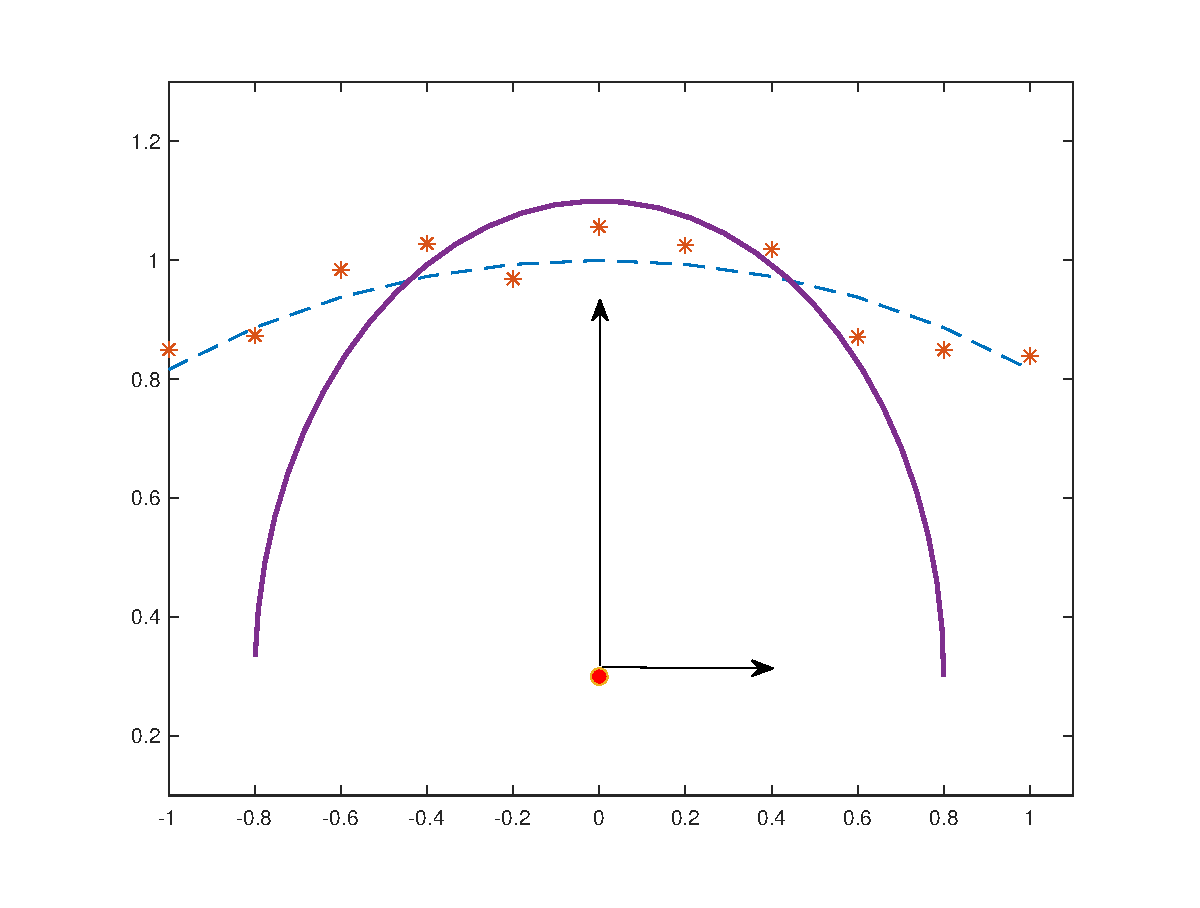
\includegraphics[width=0.32\linewidth]{../figures/demo1.eps} 
%\hspace{-4mm}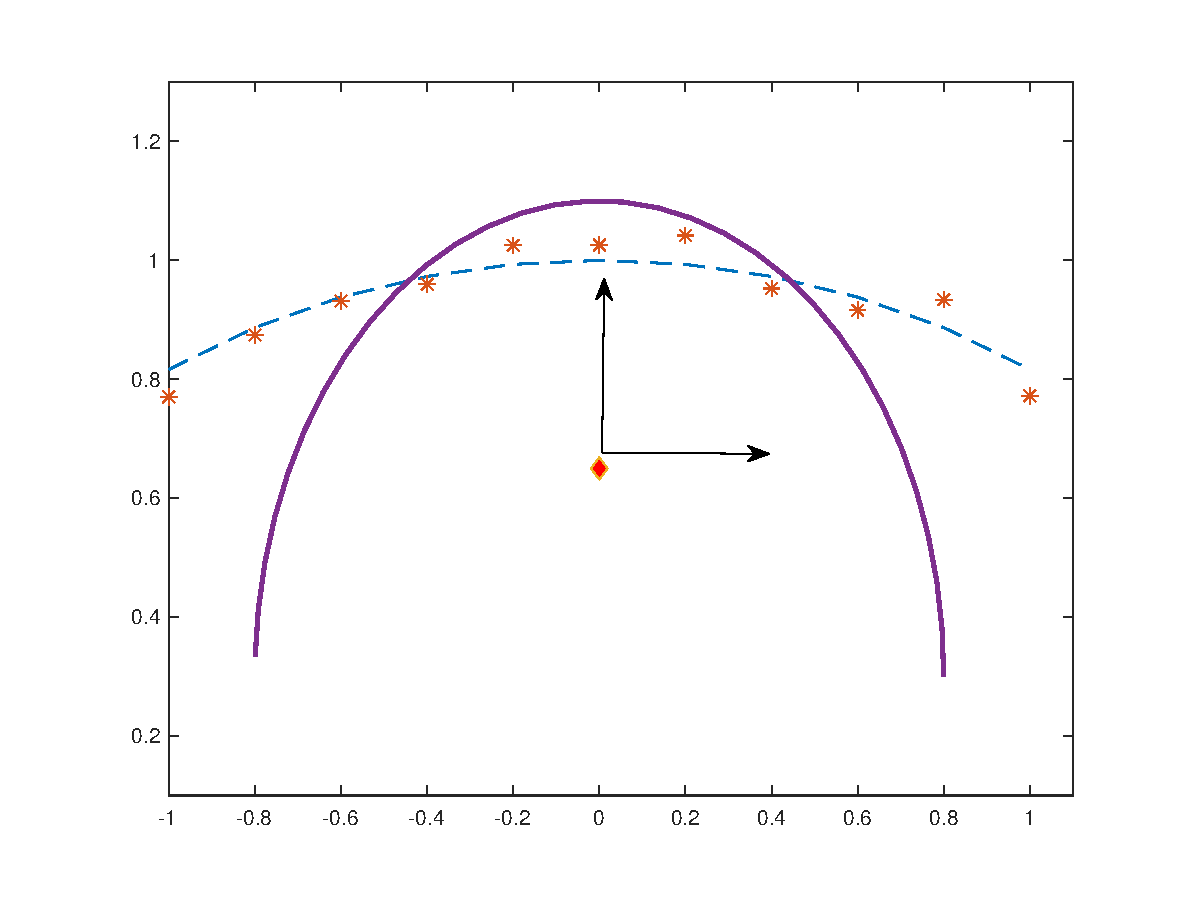
\includegraphics[width=0.32\linewidth]{../figures/demo2.eps} 
%\hspace{-4mm}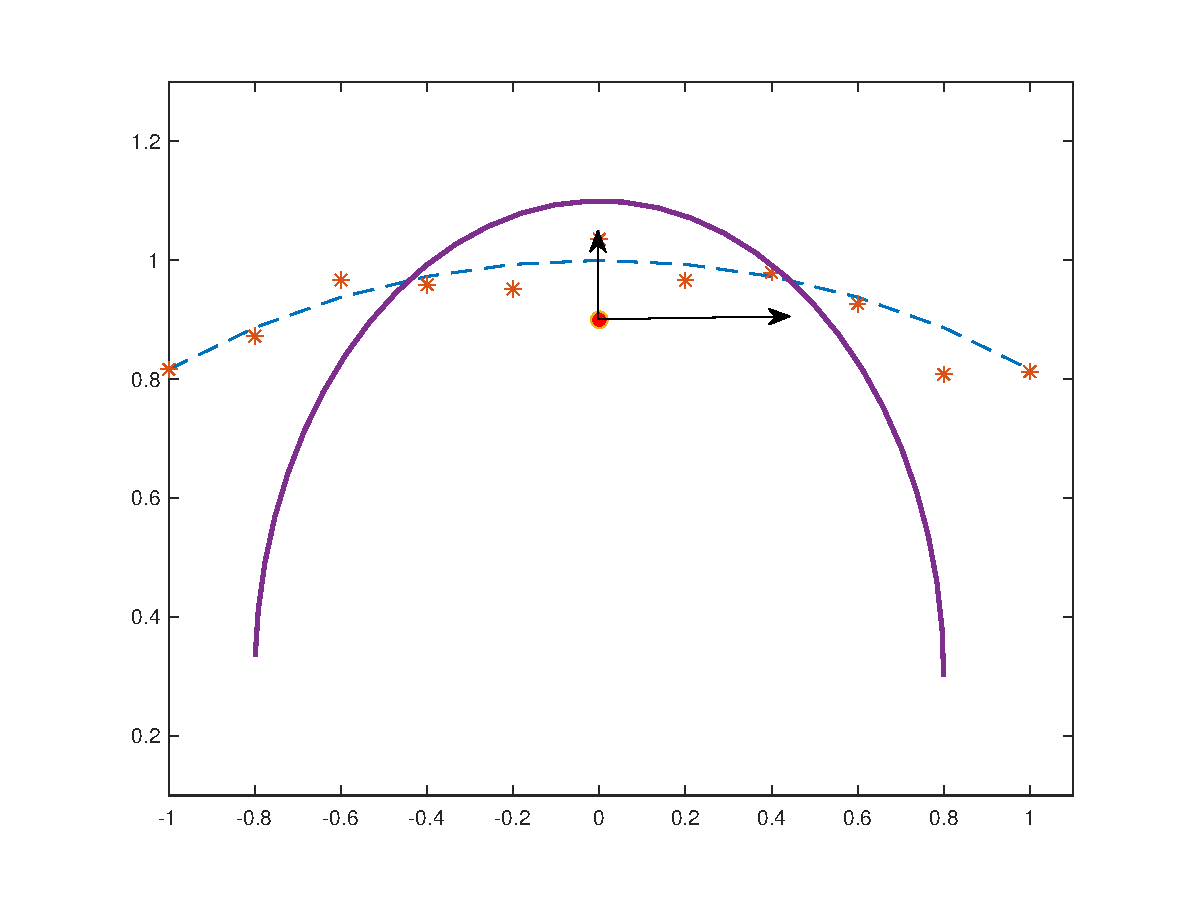
\includegraphics[width=0.32\linewidth]{../figures/demo3.eps} 
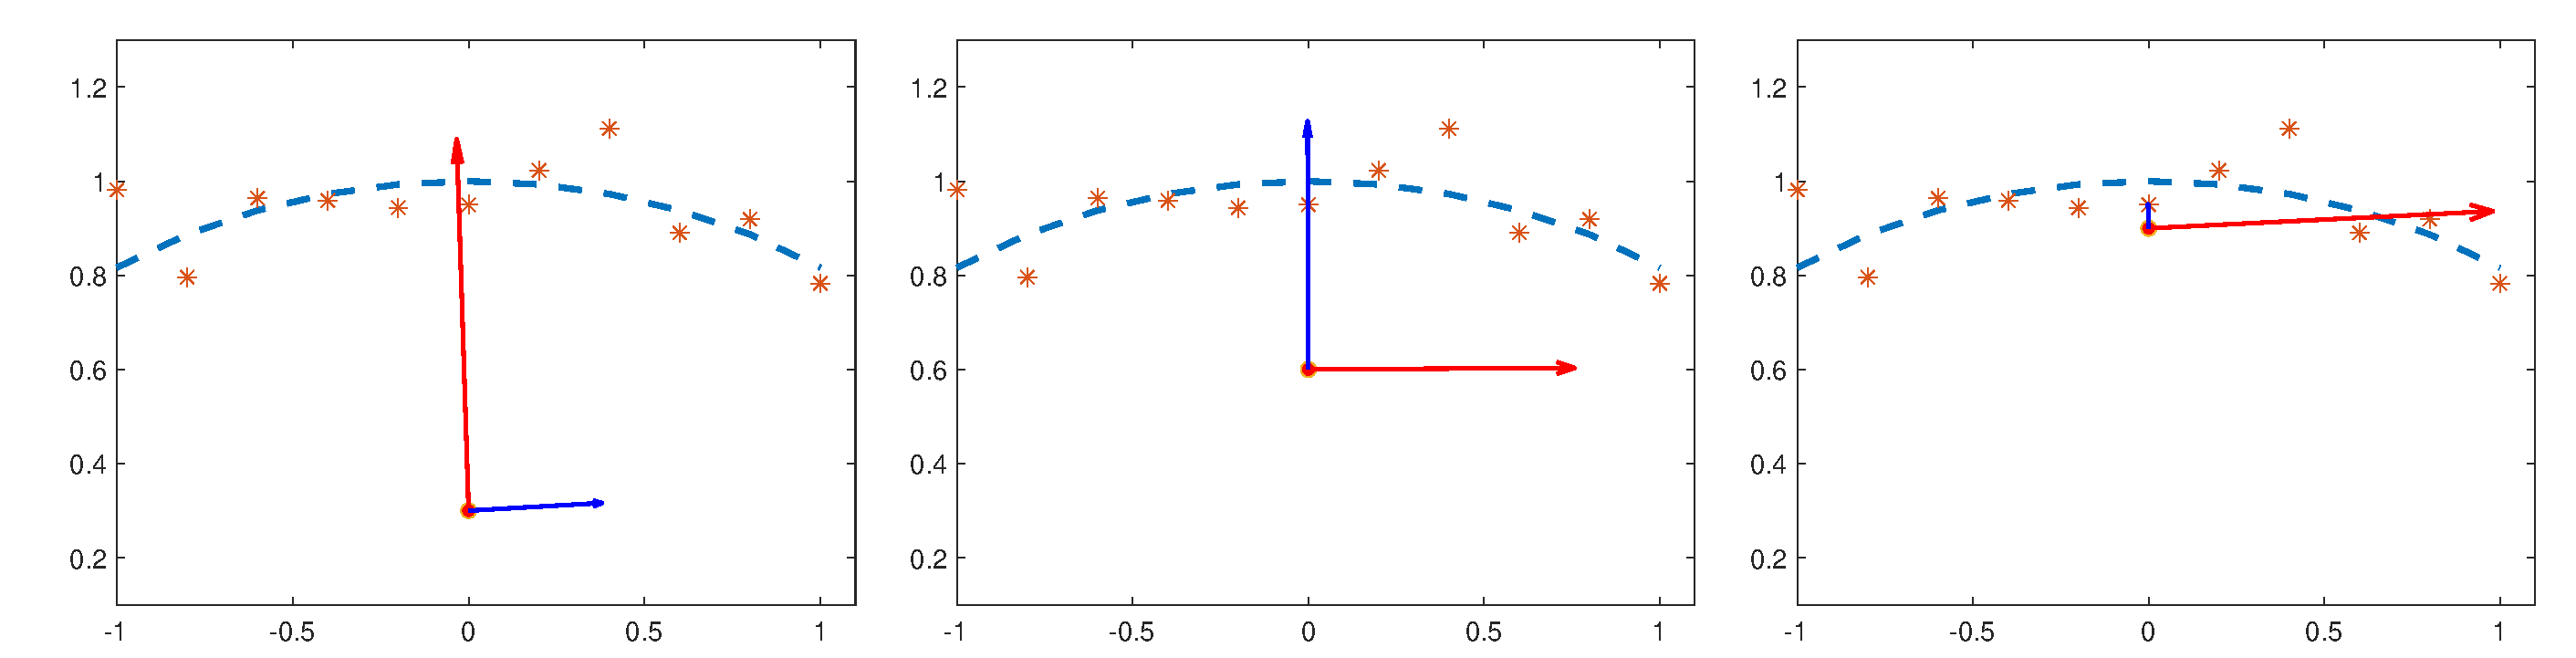
\includegraphics[width=\linewidth]{demo123.eps} 
%\setcaptionwidth{6in}
\caption{The process of the variation of $J_r(x)$'s eigenspace, with $x$ approaching the manifold }
\label{Shifting Eigenvectors}
\end{figure}

The left diagram in the figure shows that, when $x$ is far away from the data points, the space spanned by the principal eigenvectors of $J_r(x)$ resides approximately in the normal space of the manifold. As $x$ comes near the ridge, we can see that the two eigenvalues of $J_r(x)$ will be equal, as shown in the middle diagram. If $x$ continues to approach the ridge, the principal eigenvector will become parallel with the ridge.

The subspace-constrained shifting method requires $x$ to move in the normal space of the manifold to get the projection $x^*$ of $x$ onto the manifold. However, as $x$ is far away from the manifold and $x^*$ is unknown, to overcome this difficulty we can use the space spanned by the eigenvectors of $J_r(x)$, corresponding to some particular eigenvectors, as an approximation of the normal space at $x^*$. We show that this may cause some error because, as $x$ approaches the manifold, the magnitude of $\lambda_d/\lambda_{d+1}$ will change dramatically. Thus, picking the eigenvector corresponding to the largest eigenvalue may cause a sudden turn in the orthogonal direction. The unpredictable directional behavior of the principal eigenvector of $J_r(x)$ causes the searching lower-dimensional ridge algorithm to converge badly. Fortunately, this difficulty can be overcome by using a nonlinear transformation, as introduced in the next section. Through modification with a rank-one matrix, we can obtain a new $J_r(x)$ with a very stable eigenspace, i.e. the order of the first and second eigenvectors will not be reversed with the moving of $x$. %A simple two-dimensional example is provided below to illustrate this.
%The discussion can be split into three cases, depending on the relationship between $x$ and $\{x_i, i=1:N\}$.



\subsection{Eigenspace Analysis for $C_r(x)$ and $J_r(x)$}


Since the convex combination of samples in ${\cal I}_r$ spans a convex hull next to $\cal M$, $c_r(x)$ is in the convex hull, which is supposed to be next to $\cal M$ as well when $r$ is relatively small.
We prefer to use the eigenvectors corresponding to the $d$ principal eigenvalues of $C_r(x)$, instead of $J_r(x)$, to approximate the tangent space. The reasons for this will be explained in detail in the following section.


Recall $J_r(x)$ in \eqref{Hw}, which shares the same eigenvectors with the Hessian of $\hat{p}_{r,h}(x)$. We will now determine the difference between the eigenspaces of $J_r(x)$ and $C_r(x)$. To simplify our analysis, we make the following assumption:
\begin{assumption}\label{assumption}
Assume the vector $c_r(x)-x$ is orthogonal to the subspace spanned by the eigenvectors corresponding to the top $d$ eigenvalues of the covariance matrix $C_r(x)$. %= \sum_{i\in {\cal I}_r} w_h(x, x_i) (x_i-c_r(x)) (x_i-c_r(x))^T$. 
\end{assumption}
\begin{definition}
The distance between two subspaces ${\cal V}$ and ${\cal U} $ is defined as the operator norm of the error of two projection matrices, i.e. $D({\cal V},{\cal U}) = \|P_{\cal V}-P_{\cal U}\|_2$.
\end{definition}

With Assumption \ref{assumption}, and having ${\cal V}_d (C_r(x))$ denote the eigenspace spanned by the eigenvectors corresponding to the largest $d$ eigenvalues of $C_r(x)$, we have the following theorem:
\begin{theorem}
If $\|c_r(x)-x\|_2^2< \lambda_d(C_r(x)))$, the eigenspaces corresponding to the top $d$ eigenvalues of $C_r(x)$ and $J_r(x)$ coincide, i.e. the distance 
\[
D({\cal V}_d (C_r(x)), {\cal V}_d (J_r(x)))=0.
\]
Otherwise, if $\|c_r(x)-x\|_2^2\geq \lambda_d(C_r(x)))$, then 
$
D({\cal V}_d (C_r(x)),{\cal V}_d (J_r(x)))=1.
$
\end{theorem}
The details of the proof can be found in the supplementary material.

\subsection{The Singular-Point Phenomenon}
Here, we use the term `singular point' to refer to the points that satisfy the ridge condition but are obviously not on the ridge.
Suppose there exists $x_0$ such that $\|c_r(x)-x\|_2^2>\lambda_d(J_r(x_0))$, $c_r(x_0)-x_0$ is in the space ${\cal V}_d(J_r(x))$, which is spanned by the eigenvectors corresponding to the top $d$ eigenvalues of $J(x)$, and thus $c_r(x_0)-x_0\perp {\cal V}_{D-d}(J_r(x))$. In this case, applying the subspace-constrained mean-shift algorithm 
\[
x_0' = x_0+ (I-P({\cal V}_d(J_r(x)))) (c_r(x_0)-x_0)
\] 
cannot move $x_0$ because of $(I- P({\cal V}_d(J_r(x)))) (c_r(x_0)-x_0)=0$. This phenomenon will be demonstrated in Figure \ref{Shifting Eigenvectors}. To avoid this phenomenon, we introduce the density-function transformation idea and show the inclusion relation for the ridges before and after the transformation.

The nonlinear transformation to the density function corresponds to the rank-one modification to $J_r(x)$. With a proper chosen nonnegative, increasing, and concave function, the Hessian matrix for the transformed density function will diminish the effect of the uncontrollable term $(c_r(x)-x)(c_r(x)-x)^T$ in $J_r(x)$.
%As shown in the above analysis, a better locally affine space estimation from $J(x)$ requires us to reduce the perturbation effect of the rank-one matrix $(c_r(x)-x)(c_r(x)-x)^T$. Next, we introduce the density-function transformation idea, which provides a way to make a rank-one modification to $J(x)$.
\subsection{Ridge Variation via Transformation}
%\subsubsection{Density Transformation}
In this section, we show that the transformation of the estimated density function by a monotonously increasing function, $f$, will result in a new ridge $R({f(p}(x)))$, which is a subset of $R({p}(x))$. In the following calculations, we can abbreviate $R({f(p}(x)))$ and $R({p}(x))$ as $R({f(p}))$ and $R({p})$, respectively.

For two ridges defined by the density $p(x)$ and $f(p(x))$, where $f(y)$ is a monotonously increasing and concave function satisfying $f'(y)>0$ and $f''(y)<0$, we have 
\begin{equation}\label{derivatef}
\begin{aligned}
&\nabla f(p(x)) = f'(p(x)) \nabla p(x),\\
&H_{f(p)}(x) = f''(p(x)) \nabla p(x) \nabla^T p(x) + f'(p(x)) H_{p}(x).
\end{aligned}
\end{equation}
Let the d-dimensional ridges $R(p)$ and $R(f(p))$, corresponding to $p(x)$ and $f(p(x))$, be defined as
\[
\begin{aligned}
&R({p}) = \{x | \Pi_{H_{p}}^{\perp} (x) \nabla p(x) = 0, \lambda_{d+1}(H_{p}(x))<0\}, \\
&R({f(p)}) = \{x | \Pi_{H_{f(p)}}^{\perp} (x) \nabla f(p(x)) = 0,\lambda_{d+1}(H_{f(p)}(x))<0\}.
\end{aligned}
\]
%\subsubsection{Connections for the Ridges}
Next, we will provide two lemmas to show the relationship between the ridges before and after transformation:
\begin{itemize}
\item[1.]  If $\lambda>0$, a rank-one modification expressed as $\lambda uu^T$ will enlarge the projection of $u$ onto the eigenspace corresponding to the largest $d$ eigenvalues. 
\item[2.] For a rank-one modification expressed as $\lambda uu^T$, if $u$ is in some subspace spanned by the largest $d$ eigenvectors and $\lambda>0$, the rank-one modification will keep the eigenvalues corresponding to the orthogonal complement space unchanged.
\end{itemize}
These two lemmas are aligned with our intuition to some degree, which is a key step in proving the inclusion property of ridges.

\begin{lemma}{ For any symmetric matrix $B$, let $A = B +\lambda uu^T, \forall \lambda\geq 0$. We have $\|\Pi_A u\|_2\geq \|\Pi_B u\|_2$, where $\Pi_A, \Pi_B$ are the projections onto the space spanned by the eigenvectors corresponding to the $d$ largest eigenvalues of $A$ and $B$, respectively.} \label{projection_enlarge}
\end{lemma}

\begin{lemma}\label{eigvenvalue}
For any symmetric matrix $B$, let $A = B+\lambda u u^T$,  $\forall \lambda \geq 0$ and any nonzero vector $u\in  {\rm span}\{ u_1(B(x)), u_2(B(x)),..., u_d(B(x))\}$; the $(d+1)$-th  to $D$-th largest eigenvalues of $A$ and $B$ yield 
\[
\lambda_{d+k}(A) = \lambda_{d+k}(B),\quad k=1,...,D-d,
\]
where $u_k(B(x))$ and $\lambda_k(B(x))$ are the eigenvector and eigenvalue corresponding to the $k$-th largest eigenvalues of $B(x)$.
%where ${\cal S}_d = {\rm span}\{ u_1(B(x)), u_2(B(x)),..., u_d(B(x))\}$
\end{lemma}
The details of the proof of Lemma \ref{projection_enlarge} and Lemma \ref{eigvenvalue} are in the supplementary material. %appendix \ref{Rank-one Enlarge Projection}. 
\begin{remark}
Lemma \ref{projection_enlarge} is a key step in this section, as it shows that the rank-one modification $\lambda uu^T$ will enlarge the projection of $u$ onto the space spanned by the component eigenvectors.
\end{remark}
\begin{remark}
Lemma \ref{eigvenvalue} shows that the semi-positive rank-one modification in the subspace corresponding to the largest $d$ eigenvalues will keep the remaining eigenvalues corresponding to the orthogonal complement subspace unchanged.
\end{remark}
Using Lemma \ref{projection_enlarge} and Lemma \ref{eigvenvalue}, we obtain Lemma \ref{monotonously theorem}:
\begin{lemma}{
For any monotonously increasing and concave function $f(y)$, i.e. $f'(x)>0, f''(x) \leq 0$, for $x\in R({f(p)})$, the following are satisfied simultaneously:
 \begin{gather*}
 \lambda_{d+1}(H_p(x)) < 0,\\
\|\Pi_{H_p}^\perp(x)\nabla p(x)\|_2 \leq \|\Pi_{H_{f(p)}}^{\perp}(x)\nabla p(x)\|_2=0,
%\frac{1}{f'(p(x))}( \lambda_{d+1} (H_{f(p)}(x))-{f''(p(x))}\|\nabla p(x)\|_2^2)\leq 0
\end{gather*}
The condition $\|\Pi_{H_p}^\perp(x)\nabla p(x)\|_2  =0$ implies $\Pi_{H_p}^\perp(x)\nabla p(x)=\bf 0$, which in turn indicates that $x\in R(p)$. Thus, $R(f(p)) \subset R(p)$}. %, where $p(x)$ is a twice-differentiable density function.
%\label{rankonetheorem}
\label{monotonously theorem} 
\end{lemma}

The details of the proof of lemma \ref{monotonously theorem} can be found in the supplementary material. %appendix \ref{monotonously theorem proof}.
\remark{
The inclusion property $R(f(p)) \subset R(p)$ is applicable to any density function $p(x)$. When $p(x)$ is selected to be the special formate at $\hat{p}_{r,h}(x)$, we will obtain the following results by applying Lemma \ref{monotonously theorem} to the local density function $\hat{p}_{r,h}(x)$:
}

\begin{theorem}\label{inclusion}
For any monotonously increasing and concave function $f(y)$, we have $R({f(\hat{p}_{r,h})}) \subset R({\hat{p}_{r,h}})$. Furthermore, 
\[
\|\Pi_{H_{\hat{p}_{r,h}}}^\perp(x)\nabla \hat{p}_{r,h}(x)\|_2 \leq \|\Pi_{H_{f(\hat{p}_{r,h})}}^{\perp}(x)\nabla \hat{p}_{r,h}(x)\|_2.
\]
\end{theorem}

Numerically, we can set some small number $\epsilon$ such that at least $10^{-6}$ will act as a threshold for searching the ridge condition, because of the rounding error occurring with the computation. It can be observed that the ridge searching with a stop condition $\|\Pi_{H_{f(\hat{p}_{r,h})}}^{\perp}(x)\nabla \hat{p}_{r,h}(x)\|_2\leq \epsilon$ is stronger than that with $\|\Pi_{H_{\hat{p}_{r,h}}}^\perp(x)\nabla \hat{p}_{r,h}(x)\|_2\leq \epsilon$ because of the existing inequality in Theorem \ref{inclusion}.
%\begin{theorem}{$Haus(R_f, R) \leq Haus(R_p, R)$}
%\[
%Haus(X, Y) := \max\{\sup_{x\in X}\inf_{y\in Y} \|x-y\|_2, \sup_{y\in Y}\inf_{x\in X}\|x-y\|_2\}
%\]
%\end{theorem}
%\subsubsection{Which Point Resides in $R(p)/R(f(p))$?}

Clearly, the gradients of $p(x)$ and $f(p(x))$ only differ with a scale $f'(p(x))$. The scale difference will not affect the ridge from the ridge definition. As a consequence, we will analyze the Hessian matrices corresponding to $p(x)$ and $f(p(x))$, which will generate a difference between the ridges.

For any density function $p(x)$ and an increasing concave function $f(x)$, and taking the second derivative with respect to $x$, we have
\begin{equation}\label{hessian_fp}
H_{f(p)}(x) = f'(p(x)) H_p(x) +f''(p(x)) \nabla p(x)\nabla^T p(x)
\end{equation}
Rearranging \eqref{hessian_fp}, we have the relationship between Hessian matrices:
\begin{equation}\label{rankone2}
 H_{p}(x) =\frac{1}{ f'(p(x))} (H_{f(p)}(x) - f''(p(x))\nabla p(x) \nabla^T p(x)) .
\end{equation}
From \eqref{rankone2}, we know the rank-one modification becomes even stronger when the term $\|-f''(p(x))\nabla p(x) \nabla p^T(x)\|_F^2$ is at a larger scale. Specifically, if we select $f(y) = \log(y)$, we have $f''(p(x))=-1/p^2(x)$. Then, the rank-one modification term becomes
\[
-f''(y)\nabla p(x) \nabla p^T(x) = \frac{1}{p^2(x)} \nabla p(x) \nabla p^T(x).
\]
Note that
\[
\|-f''(y)\nabla p(x) \nabla p^T(x)\|_F^{1/2} = \frac{\|\nabla p(x)\|_2}{p(x)}.
\]
The difference between the principal eigenspaces (corresponding to the top $d$ eigenvalues) of $H_p(x)$ and $H_{f(p)}$ depends on the balance of values for $\|\nabla p(x)\|_2$ and $p(x)$.
\begin{itemize}
\item[1.] For $x$ that has large $\|\nabla p(x)\|_2$ and small $p(x)$, the rank-one modification will make a big difference.
\item[2.] For $x$ that has small $\|\nabla p(x)\|_2$ and large $p(x)$, the effect of the rank-one modification will be small.
\end{itemize}
\begin{example}
We give an example that has a large scale $\|\nabla p(x)\|_2/p(x)$, estimating $\hat{p}(x)$ using the KDE function with a form of 
\[
\hat{p}(x):=  \frac{1}{n} \sum_i K(-\|x-x_i\|_2^2/h^2).
\]
Then, $\|\nabla \hat{p}(x)\|_2/\hat{p}(x)$ has a geometry interpretation as the distance from $x$ to a point in the convex hull
\[
\frac{\|\nabla \hat{p}(x)\|_2}{\hat{p}(x)} = \frac{2}{h^2} \|c_r(x)-x\|_2,
\]
where $c_r(x)$ is defined in \eqref{c_r_x} as a point
%\[
%\|-f''(y)\nabla \hat{p}(x) \nabla \hat{p}^T(x)\|_F = \|\frac{4}{h^4}  (c_r(x) - x) (c_r(x) - x)^T\|_F = \frac{4}{h^4} \|c_r(x)-x\|_2^2.
%\]
%A convex weighted summation of $\{x_i\}$, it resides 
in the convex hull of $\{x_i, i\in I_r\}$. For any $x\not \in {\rm Conv}\{x_i, i\in I_r \}$, the distance $\|c_r(x) -x\|_2$ has a lower bound:
\[
\|c_r(x) -x\|_2 \geq \|{ P}_{\rm Conv} (x) -x\|_2 = \|{ P}^{\perp}_{\rm Conv} x\|_2,
\]
where ${P}_{\rm Conv}(x)$ is the projection of $x$ into the convex hull. %of samples $\{x_i, i\in {\mathcal I}_r\}$. 
As the initial point $x:=x_0$ could be any point away from the convex hull, the value $\|{ P}^{\perp}_{\rm Conv} x_0\|_2$ could be at any large scale.
\end{example}
\begin{theorem}{The subtract set $R(p)/R(f(p))$ consists of points in the set:
\[
\{ x | c_r(x) - x \in {\rm span} \{u_1,...,u_d\}, c_r(x) - x \not \in {\rm span} \{v_1,...,v_d\}\},
\] 
where $\{u_1,...,u_d\}$ and $\{v_1,...,v_d\}$ are the eigenvectors corresponding to the top $d$ eigenvalues of $H_p(x)$ and $H_{f(p)}(x)$}, respectively. 
\end{theorem}
\begin{remark}
The points in $R(p)/R(f(p))$ are often far from our intended ridge. Neglecting this group of points will yield a ridge much closer than before.
\end{remark}
%As in real cases, $R/R_f$ consists only of a relatively small portion of $R$. Applying KDE with $\log(p(x))$ instead of $p(x)$ will not improve the performance very much. Next, we perform a deep analysis of the relationship between the Hessian and tangent-space estimation, and propose a new way to improve our ridge-estimation method.
We demonstrate that the ridge obtained from the nonlinear transformation can indeed be closer than the original one by showing that ${\rm Haus} (R(f(p)), {\cal M}_{R(f(p))})$ is smaller than ${\rm Haus} (R(p), {\cal M}_{R(p)})$.
\begin{theorem}\label{Transformed Inequality Theorem}
For the ridge $R(f(p))$ defined by the transformed nonlinear increasing and concave function $f$, we have
\[
{\rm Haus} (R(f(p)), {\cal M}_{R(f(p))}) \leq {\rm Haus} (R(p), {\cal M}_{R(p)}),
\]
where $R(p)$ and $R(f(p))$ are the $d$-dimensional ridges corresponding to $p$ and $f(p)$, and ${\cal M}_{R(p)}$ and ${\cal M}_{R(f(p))}$ are the projections of $R(p)$ and $R(f(p))$ onto $\cal M$, respectively.
%$\sup_{x\in R_f} \inf_{y\in {\cal M}_R} \|x-y\|_2 \leq {\rm Haus} (R, {\cal M}_{R})$
\end{theorem}
The proof of Theorem \ref{Transformed Inequality Theorem} can be found in the supplementary material.%appendix \ref{Transformed Inequality}.
\subsection{Geometric Interpretation}

The angle between a vector $v$ and space $\mathcal S$ is defined as the smallest angle between $v$ and $u \in \mathcal S$. Under this condition, $u$ is the projection of $v$ onto the space of $\mathcal S$, i.e. $u = { P_{\mathcal S}}(v)$.
\[
\theta(v, {\mathcal S}) = \arg \cos \frac{\langle v, {P}_{\mathcal S} v\rangle }{\|v\|_2 \|{P}_{\mathcal S} v\|_2} =   \arg \cos( \| P_{\mathcal S} v\|_2 / \|v\|_2 ).
\]
Let ${\mathcal S}_{H_p}$ and ${\mathcal S}_{H_{f(p)}}$ denote the spaces spanned by the eigenvectors corresponding to the top $d$ eigenvalues of $H_p(x)$ and $H_{f(p)}(x)$, respectively.
 
 From Lemma \ref{monotonously theorem}, we know
 \begin{equation}\label{relationHF}
 \nabla p(x)^T \Pi_{H_p}(x) \nabla p(x)\geq \nabla p(x)^T \Pi_{H_{f(p)}}(x) \nabla p(x).
 \end{equation}
 The inequality \eqref{relationHF} indicates $\| \Pi_{H_p}(x) \nabla p(x)\|_2 \geq  \|\Pi_{H_{f(p)}}(x) \nabla p(x)\|_2$, which is equivalent to 
 \begin{equation*}\label{angle_ineq}
\cos( \theta(\nabla p(x), {\mathcal S}_{H_p})) = \frac{\| \Pi_{H_p}(x) \nabla p(x)\|_2}{\|\nabla p(x)\|_2} 
\geq  \frac{\|\Pi_{H_{f(p)}}(x) \nabla p(x)\|_2}{\|\nabla p(x)\|_2} = \cos(\theta(\nabla p(x), {\mathcal S}_{H_{f(p)}})),
\end{equation*}
which implies that, for any $x$ and any increasing concave function $f$, we always have the inequality 
 \[
 \theta(\nabla p(x), {\mathcal S}_{H_{p}}(x)) \leq \theta(\nabla p(x), {\mathcal S}_{H_{f(p)}}(x)).\] 
 \remark{
The absolute value of $\cos( \theta(\nabla p(x), {\mathcal S}_{H_p}))$ stands for the size of the angle between the vector $\nabla p(x)$ and the subspace ${\mathcal S}_{H_p}$. If $|\cos( \theta(\nabla p(x), {\mathcal S}_{H_p}))|=1$, the vector $\nabla p(x)$ is parallel with the subspace. If $|\cos( \theta(\nabla p(x), {\mathcal S}_{H_p}))|=0$, the vector $\nabla p(x)$ is vertical in relation to the subspace. If $|\cos( \theta(\nabla p(x), {\mathcal S}_{H_p}))|$ approaches $1$, this will make $x$ satisfy the ridge condition $\Pi^{\perp}(x)\nabla g(x)=0$ gradually.}

\section{Numerical Experiments}\label{experiments}
In this section, we will show the effectiveness of our method compared with the classical subspace-constrained methods for manifold fitting. The comparison is based on a uniform frame for all methods.
Overall, the manifold algorithm can be split into two parts. For the first part, for any point ${x}$ lying outside the manifold, construct an attraction force starting from ${x}$ and ending with some point (often represented by the observations) on the manifold. For the second part, estimate the normal space and use the projection to modify the attraction force such that $x$'s moving trajectory resembles the projected trajectory as much as possible. We briefly summarize the main methods considered for comparison below and we refer the readers to the Appendix \ref{Uniform_Framework}  for the implementation details (B1-B2) and the Ridge-searching Algorithm for SCRE (B3).

{\bf Implementation:} {\rm SCRE}, {\it l}-SCRE, MFIT-i \citep{fefferman2018fitting}, and MFIT-ii \citep{yao2019manifold}. The MATLAB codes together with all numerical examples used in this paper are available on \url{https://zhigang-yao.github.io/research.html} (for {\rm SCRE}, {\it l}-SCRE and MFIT-ii). We have implemented MFIT-i,  since the authors of \cite{fefferman2018fitting} have not provided implementation due to the nature of their work has been purely abstract. 


\subsection{Ridge Criteria}
The criterion for a point on a ridge is that it must satisfy the ridge condition. The ridge condition indicates that, when $x$ is on the ridge, the attraction vector $F(x)$ resides in the tangent space. The tangent space is usually obtained from the top d eigenvectors of the covariance matrix. Conversely, if the ridge condition is not met at $x$, we can also expect the angle between the attraction vector $F(x)$ and the estimated eigenspace to be large, i.e. a small cos value. 

An example of a one-dimensional curve embedded in a two-dimensional space is provided below. In this case, the tangent space and the normal space are both one-dimensional.
We first sample some points (blue circles) that represent the observations $\{x_k\}$. Then, we randomly sample the filled red diamonds that stand for $x$. The value on the figure is computed as
\[
{\rm s}(x) =  |\cos(v(x),u(x))| = |\frac{\langle v(x), u(x) \rangle}{\|v(x)\|\|u(x)\|}|,
\]
where $u(x)$ is the eigenvector corresponding to the largest eigenvalue of the covariance matrix and $v(x)$ is the gradient of the density function. Clearly, $u(x)$ is parallel with $v(x)$ when $x$ is on the manifold, i.e. ${\rm s}(x)=1$. We want ${\rm s}(x)$ to indicate the relationship between $x$ and the ridge. When ${\rm s}(x)=1$ the point $x$ should lie approximately on the ridge, and the far-away point $x$ makes ${\rm s}(x)$ approach $0$.

Different methods have different forms of attraction and projection. For brevity, we list the covariance matrices corresponding to different methods in the table below.
% \begin{table}
% 
% \resizebox{15cm}{!}{
% \begin{tabular}{c|c|c|c}\hline
% 			&KDE & KDE with $\log$ & LKDE with $\log$\\\hline
%Attraction&$c(x)-x$&$c(x)-x$& $c_r(x)-x$\\
% Co-Matrix& $\sum_k w(x,x_k)(x-x_k)(x-x_k)^T$&$\sum_k w(x,x_k)(c(x)-x_k)(c(x)-x_k)^T$& $\sum_{k\in I_r} w(x,x_k)(c_r(x)-x_k)(c_r(x)-x_k)^T$\\ \hline
% \end{tabular}}
% \end{table}
 
 From Figure \ref{fig:Diff Covariance}, we can draw the following conclusions:
  \begin{figure}[h] %  figure placement: here, top, bottom, or page
    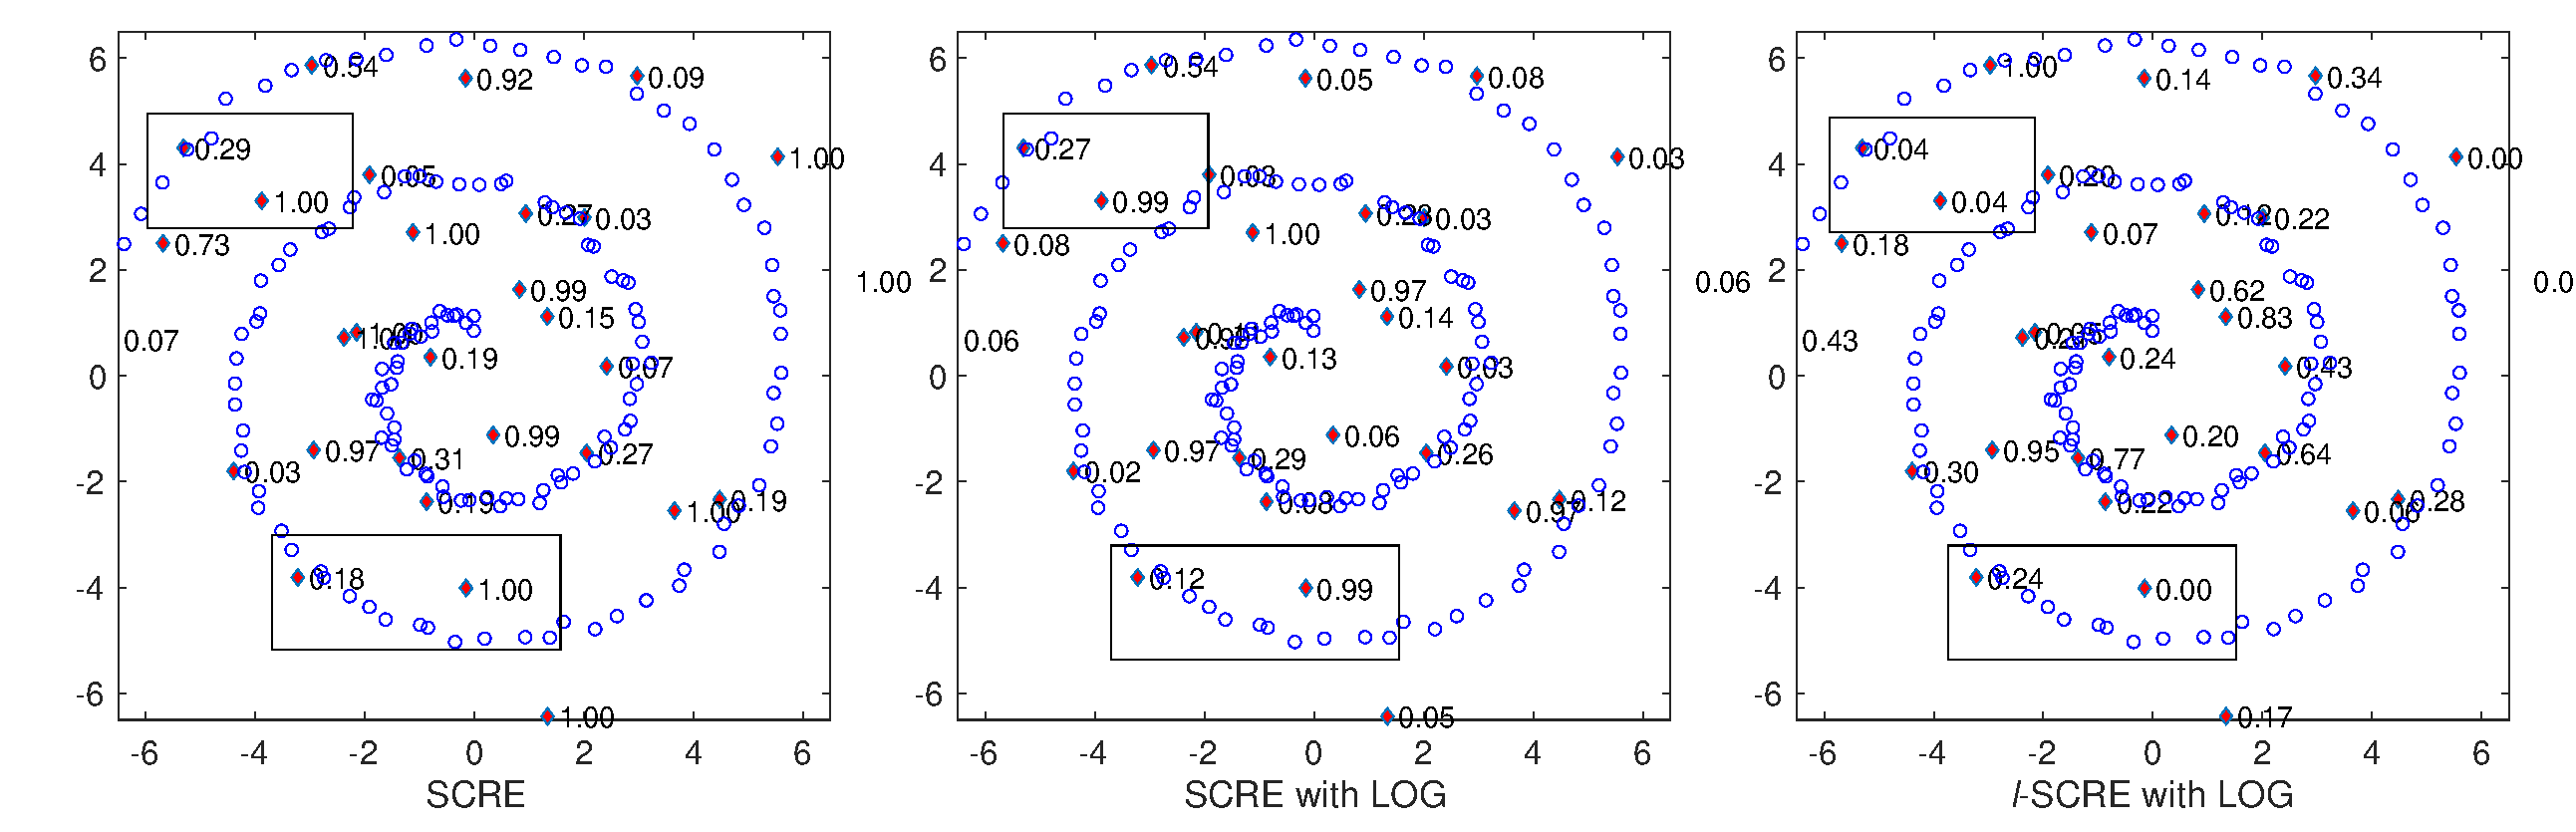
\includegraphics[width=\linewidth]{compare5n.eps} 
    \caption{Illustration of the Performances of Three Difference Covariance Matrices }
    %\setcaptionwidth{6in}
    \label{fig:Diff Covariance}
 \end{figure}
 \begin{itemize}
 \item As the left diagram shows, ${\rm s}(x)=1$ is a necessary but insufficient condition for $x$ to be on the ridge for SCRE. The outliers that are far from the ridge may also make $s(x)=1$, which is the main disadvantage of obtaining the ridge by SCRE without the nonlinear transformation.
 \item Theorem \ref{inclusion} is verified, as the values in the middle figure are uniformly smaller than the corresponding values in the left figure.
\item {\it l}-SCRE has a better property, especially for the values emphasized in the rectangle shown in the right diagram. The outlier points have much smaller values of ${\rm s}(x)$ in the right diagram than those in the former two diagrams.
 \end{itemize}
 
   \begin{figure}[h] %  figure placement: here, top, bottom, or page
    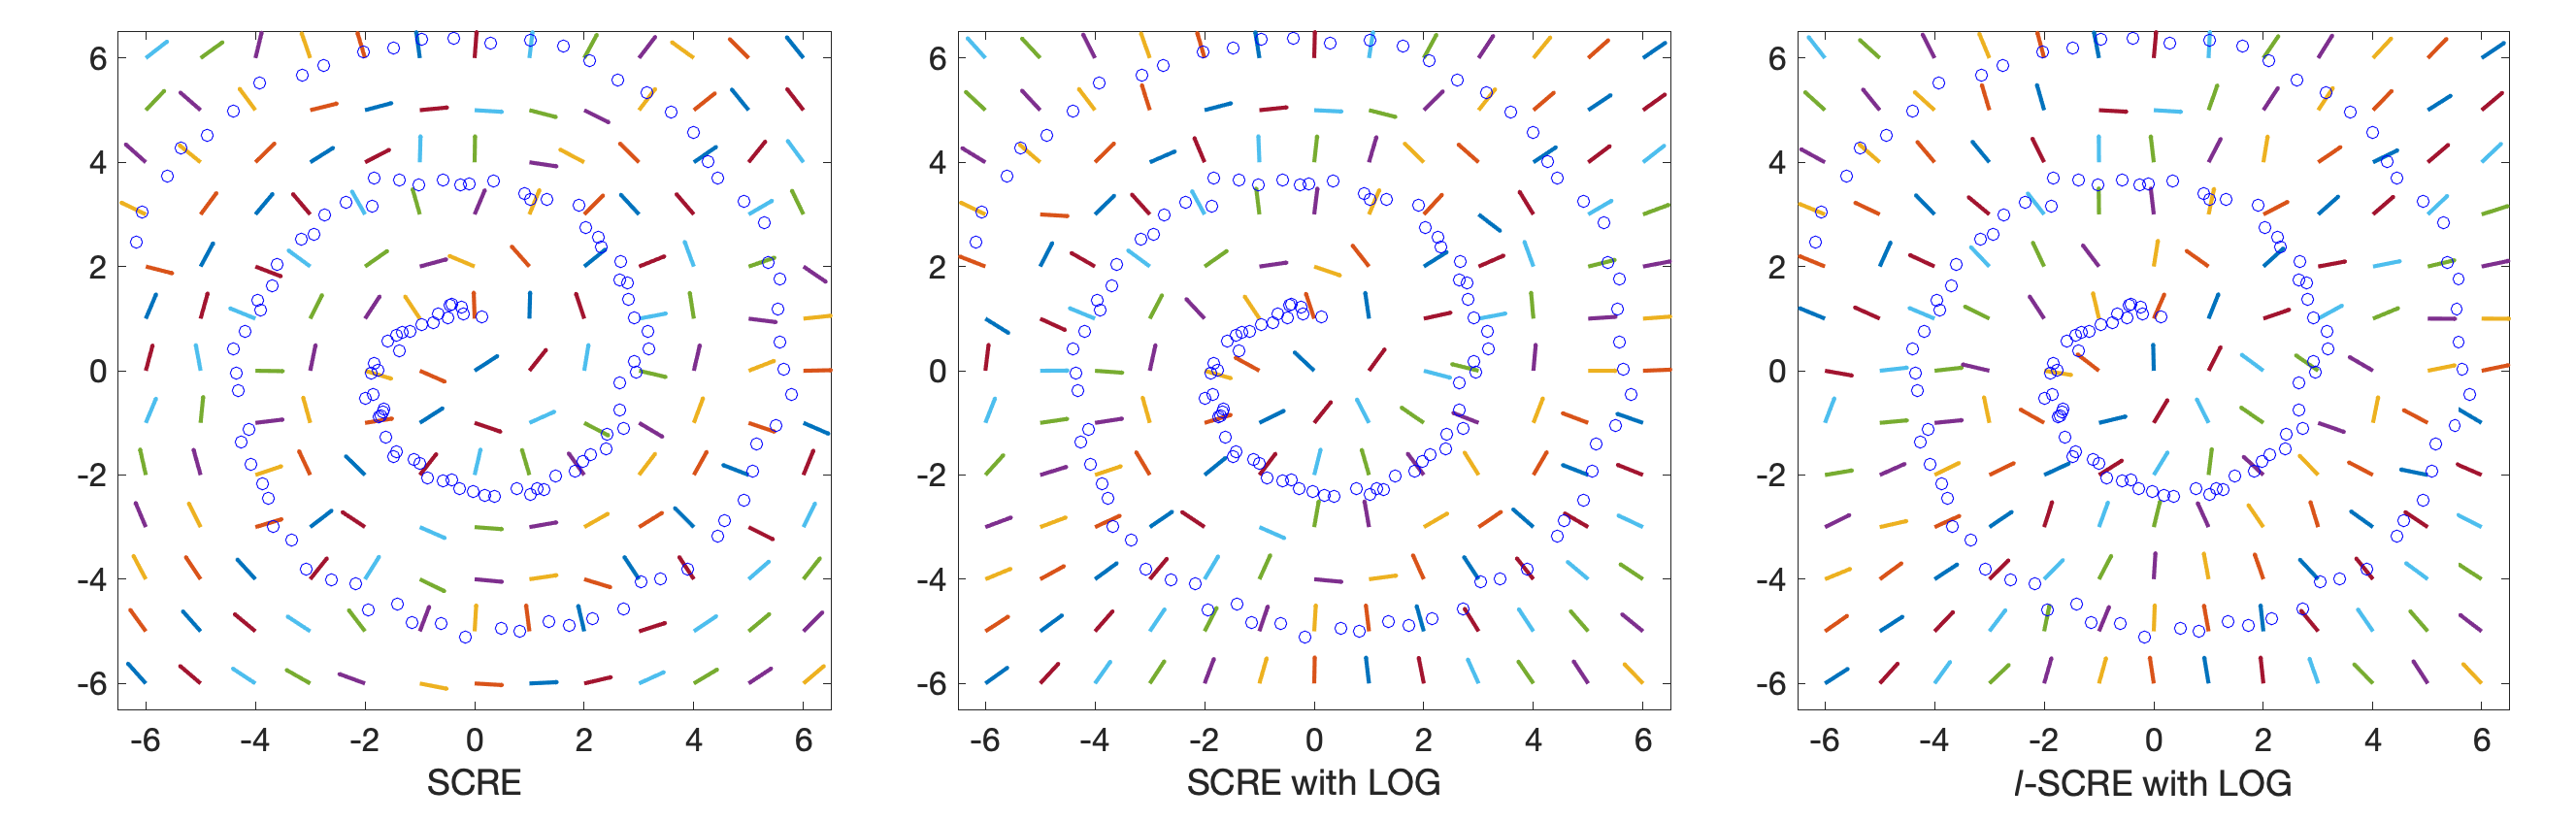
\includegraphics[width=\linewidth]{vectorfield2.eps} 
    % \setcaptionwidth{6in}
    \caption{Illustration of the vector field corresponding to the eigenvector of the second eigenvalue with respect to three difference covariance matrices }
    \label{fig:vectorfield}
 \end{figure}
In Figure \ref{fig:vectorfield}, we plot the vector field generated by the eigenvector corresponding to the smallest eigenvalue. This vector field is the geometric interpretation of the projection $\Pi^{\perp}$ in the two-dimensional space. Because the constrained subspace in the two-dimensional space is one-dimensional, the vector field coincides with the trajectory of the outliers moving onto the ridge. We can conclude from the above figures that the vector field corresponding to {\it l}-SCRE is more smooth and points approximately to the projection onto the manifold, while the vector field of SCRE is not well behaved for samples not close to the manifold.
\subsection{Synthetic Data Set}
First, we provide a one-dimensional ring example to show the effectiveness of our method compared with SCRE. Because of the simplicity of the circle structure, it is easy to compute the real projection onto it. We assume that our hidden manifold ${\mathcal M}$ is the one-dimensional circle embedded in a two-dimensional space with a radius of $1$ and center of $(0,0)$.

The observations are generated in the following two steps. First, a uniform sample from ${\mathcal M}$ is used to obtain the ideal observations without noise $\tilde{y}_i, i = 1:N$. Second, the independent noise from a two-dimensional normal distribution is added to get $y_i = \tilde{y}_i+\epsilon_i, i=1:N$. The observations are used to construct our SCRE and {\it l}-SCRE functions.

Generate a random mesh set $\mathcal G$ arbitrarily. For each point $x_k \in \mathcal G$, apply the subspace-constrained mean-shift algorithm to obtain a point $\hat{x}_k$ that satisfies the ridge definition. Thus, the computed ridge set is ${\cal \hat{G}}=\{\hat{x}_k\}$. Because we use different approaches to define our ridge sets, we have ${\cal \hat{G}}$ and ${\cal \hat{G}}_\ell$, which correspond to the SCRE and {\it l}-SCRE approaches.

For each point $\hat{x}$ belonging to ${\cal \hat{G}}$ or ${\cal \hat{G}}_\ell$, we can define the projection of $\hat{x}$ onto the real manifold $\mathcal M$ as $\pi_{\mathcal M}(\hat{x}) = \arg\min_{y\in \mathcal M} \|y-\hat{x}\|_2$. In the case of the special two-dimensional circle, the projection has an explicit form, $\pi_{\mathcal M}(\hat{x}) = \hat{x}/\|\hat{x}\|$. The average margin from $\cal \hat{G}$ or ${ \cal \hat{G}}_\ell$ to $\mathcal M$ is defined as
\[
{\rm Margin}({ \cal \hat{G}, \mathcal M}) =\frac{1}{|{\cal \hat{G}}|}  \sum_{x_k\in  {\cal \hat{G}}} \min_{y\in \mathcal M}\|x_k-y\|_2.
\]
\begin{figure}[t] %  figure placement: here, top, bottom, or page
   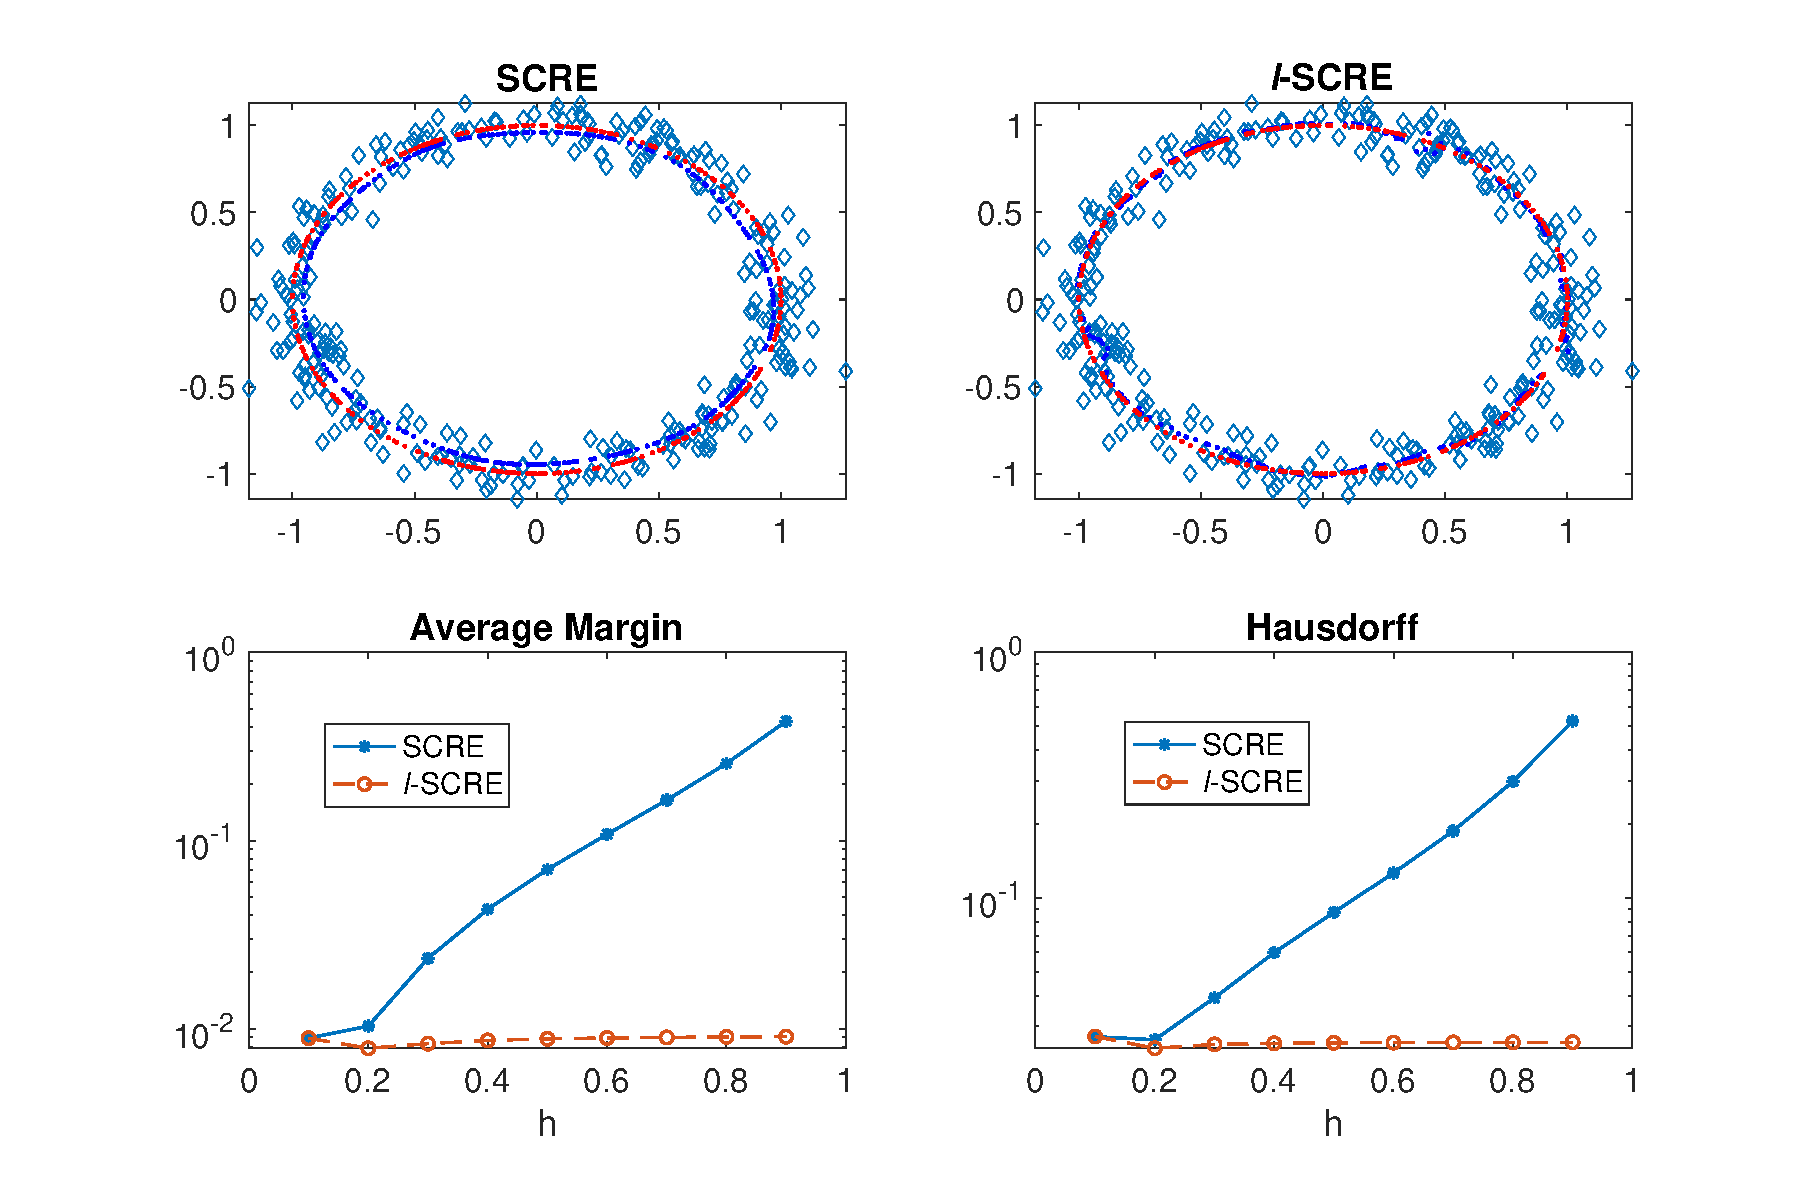
\includegraphics[width=\linewidth]{circle8n.eps} 
   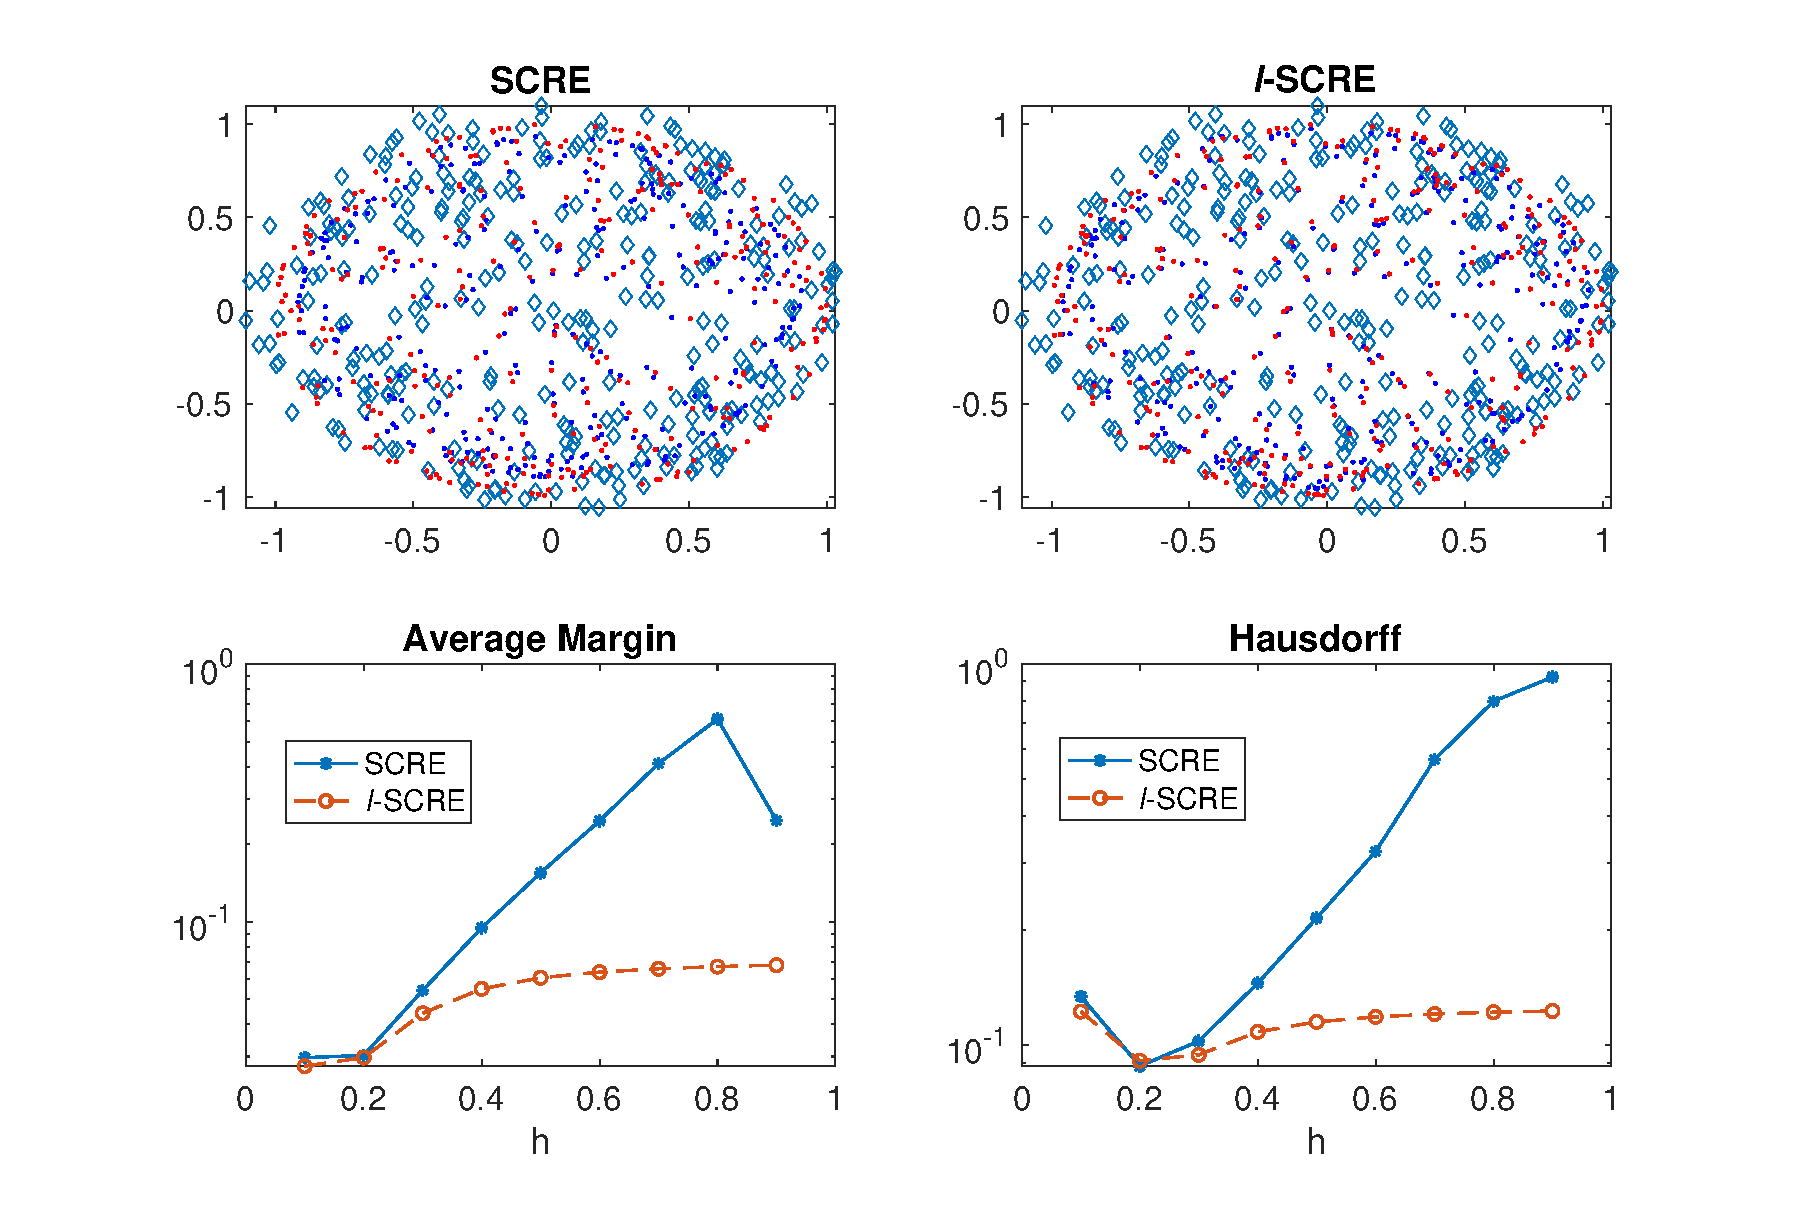
\includegraphics[width=\linewidth]{sphere8.eps} 
   %\setcaptionwidth{6in}
   \vspace{-1cm}
   \caption{Margin and Hausdorff illustration for ridges obtained from {\it l}-SCRE and SCRE}
   \label{fig:circle6}
\end{figure}

In Figure \ref{fig:circle6}, the small blue diamonds $\diamond$ represent the observations that are used to construct our SCRE or {\it l}-SCRE estimator. The blue dots $\bullet$ represent the points that satisfy the ridge condition. The red dots $\bullet$ represent the projection of the blue dots onto the ideal manifold ${\mathcal M}$.

For the above two figures, the margin of the ridge corresponding to SCRE is shown in the left partition and the margin of the ridge corresponding to {\it l}-SCRE is shown in the right partition.
In the two figures below, we show how the average margin and Hausdorff distance, between $\cal \hat{G}$ and ${\cal M}_{\cal \hat{G}}$, change with the parameter $h$ when the neighborhood size parameter is fixed.

%\begin{table}[h]
%\caption{The margin and Hausdorff between $\cal \hat{G}$ and ${\cal \hat{G}}_{\ell}$. $\mathcal M$ varies with $h$ for SCRE and {\it l}-SCRE}.
%\resizebox{14cm}{!}{
%\begin{tabular}{c|c|ccccccccc}\hline
%  & $h$   & 0.1   &0.2 &0.3 &0.4&0.5&0.6&0.7&0.8&0.9\\\hline
% \multirow{2}{*}{Marg} &SCRE  & 0.0121 &   0.0123 &   0.0246 &   0.0445  &  0.0716 &   0.1091 &   0.1648  &  0.2565 &   0.4274 \\ 
%  &{\it l}-SCRE &  0.0118 &   0.0120 &   0.0182 &   0.0225 &   0.0249 &   0.0264 &    0.0272 &    0.0278 &   0.0283 \\ \hline
% \multirow{ 2}{*}{Haus} &SCRE  &  0.0779 &   0.0333 &   0.0468 &   0.0662 &   0.0913 &   0.1307 &   0.1881 &   0.2837  &  0.4765 \\ 
% &{\it l}-SCRE & 0.0492 &   0.0329 &   0.0408 &   0.0456 &   0.0489  &  0.0510 &   0.0524 &   0.0534 &   0.0540 \\ \hline
%\end{tabular}}
%\label{table:margin}
%\end{table}

It is clear from Table \ref{result_compare} and Figure \ref{fig:circle6} that, under the same parameter setting (such as $h$ and noise level $\sigma$), the algorithm of {\it l}-SCRE yields a ridge with a margin much smaller than that of SCRE. The rate of increase of the distance measurement for {\it l}-SCRE is much lower than that for SCRE with the increasing $h$. This phenomenon is also explained in our theoretical analysis.

\begin{table}[h]
\caption{The margin and Hausdorff between $\cal \hat{G}$ and $\mathcal M$ vary with $h$ for SCRE, {\it l}-SCRE, MFIT-i and MFIT-ii on the 1-dimensional circle}.
\resizebox{14cm}{!}{
\label{result_compare}
\begin{tabular}{c|c|ccccccccc}\hline
  & $h$   & 0.1   &0.2 &0.3 &0.4&0.5&0.6&0.7&0.8&0.9\\\hline
  \multirow{4}{*}{Marg}  &SCRE 
& 0.0089 & 0.0103 & 0.0237 & 0.0431 & 0.0702 & 0.1080 & 0.1642 & 0.2569 & 0.4307 \\
  &{\it l}-SCRE
 & 0.0089 & 0.0079 & 0.0083 & 0.0087 & 0.0088 & 0.0089 & 0.0090 & 0.0090 & 0.0091 \\
  &MFIT-i
& 0.0240 & 0.0092 & 0.0076 & 0.0087 & 0.0134 & 0.0200 & 0.0276 & 0.0367 & 0.0473 \\
  &MFIT-ii
& 0.0263 & 0.0113 & 0.0107 & 0.0119 & 0.0155 & 0.0210 & 0.0278 & 0.0356 & 0.0438 \\
  \hline
\multirow{4}{*}{Haus}  &SCRE
& 0.0272 & 0.0265 & 0.0392 & 0.0599 & 0.0875 & 0.1264 & 0.1875 & 0.2979 & 0.5251 \\
  &{\it l}-SCRE
& 0.0273 & 0.0244 & 0.0253 & 0.0256 & 0.0257 & 0.0258 & 0.0258 & 0.0258 & 0.0259 \\
  &MFIT-i
& 0.1164 & 0.0278 & 0.0242 & 0.0260 & 0.0282 & 0.0351 & 0.0443 & 0.0544 & 0.0650 \\
  &MFIT-ii
 & 0.1165 & 0.0461 & 0.0252 & 0.0261 & 0.0332 & 0.0412 & 0.0494 & 0.0583 & 0.0710 \\
 \hline
\end{tabular}}
\end{table}

\begin{table}[h]
\caption{The margin and Hausdorff between $\cal \hat{G}$ and $\mathcal M$ vary with $h$ for SCRE, {\it l}-SCRE, MFIT-i and MFIT-ii on the 2-dimensional sphere}.
\resizebox{14cm}{!}{
\label{result_compare}
\begin{tabular}{c|c|ccccccccc}\hline
  & $h$   & 0.1   &0.2 &0.3 &0.4&0.5&0.6&0.7&0.8&0.9\\\hline
  \multirow{4}{*}{Marg}  &SCRE 
& 0.0296 & 0.0304 & 0.0557 & 0.0955 & 0.1552 & 0.2478 & 0.4155 & 0.7002 & 0.3371 \\
  &{\it l}-SCRE
& 0.0274 & 0.0272 & 0.0323 & 0.0348 & 0.0360 & 0.0366 & 0.0371 & 0.0373 & 0.0375 \\
  &MFIT-i
& 0.1117 & 0.0409 & 0.0305 & 0.0228 & 0.0305 & 0.0457 & 0.0639 & 0.0849 & 0.1098 \\
  &MFIT-ii
& 0.0288 & 0.0357 & 0.0332 & 0.0285 & 0.0327 & 0.0444 & 0.0591 & 0.0763 & 0.0951 \\  \hline
\multirow{4}{*}{Haus}  &SCRE
& 0.1485 & 0.0891 & 0.0977 & 0.1303 & 0.1915 & 0.3047 & 0.5106 & 0.8972 & 0.9847 \\
  &{\it l}-SCRE
& 0.2012 & 0.0915 & 0.0799 & 0.0790 & 0.0800 & 0.0817 & 0.0827 & 0.0833 & 0.0837 \\
  &MFIT-i
& 0.9114 & 0.4856 & 0.1323 & 0.1129 & 0.0761 & 0.0849 & 0.0990 & 0.1191 & 0.1443 \\
  &MFIT-ii
& 0.1117 & 0.1201 & 0.1384 & 0.1648 & 0.1280 & 0.1146 & 0.1360 & 0.1417 & 0.1786 \\
 \hline
\end{tabular}}
\end{table}

In Table \ref{result_compare}, we provide another randomly generated circle-sample dataset. As shown in the table, when $h$ is too small (for instance in the cases shown by `-'), we cannot ensure that the domain of $x$ contains enough samples to run both MFIT-i and MFIT-ii. By comparing the margin and Hausdorff distance, we can conclude that the result of {\it l}-SCRE is more stable and competitive than the results of related methods.



\subsection{Real Data Set}
We also test the performance of our algorithm using the Coil20 \cite{Coil20} dataset. The data is collected by rotating an object with 360 degrees. For each object, there are 72 images corresponding to a particular angle. Therefore, the images for each object can be supposed to reside on a one-dimensional manifold, since the underlying parameter is the angle.

\begin{figure}[h] %  figure placement: here, top, bottom, or page
   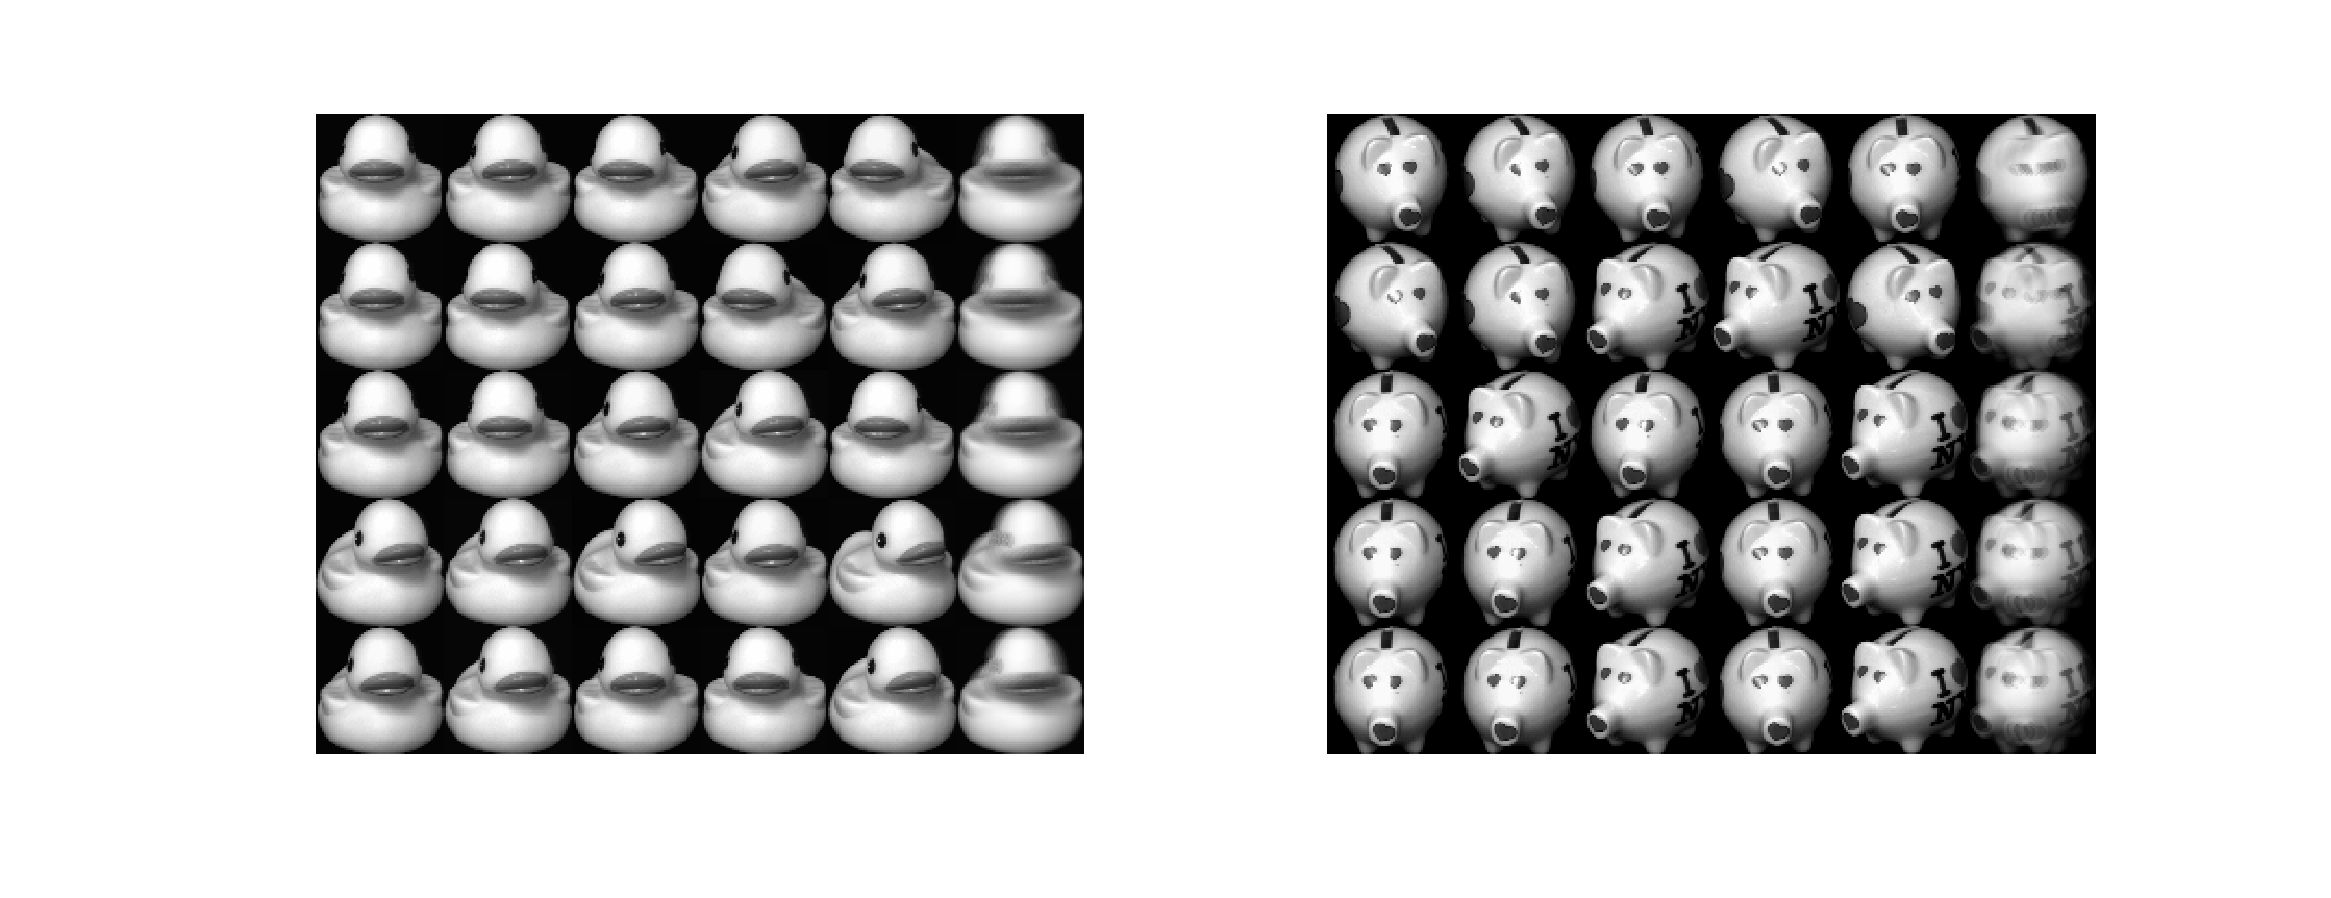
\includegraphics[width=\linewidth]{duck_pig.eps} 
   %\includegraphics[width=0.45\linewidth]{../figures/pig.eps} 
   \caption{Illustration of the interpolation for the one-dimensional Image Manifold}
   \label{fig:interpolation demo}
\end{figure}

Because we need to compute the eigenspace decomposition in the pixel space, the complexity is $O(n^3)$, where $n$ is the number of pixels. To reduce the complexity, we subsample each image with a $2\times 2$ window and obtain an image with the shape of $64\times 64$.

We randomly generate initial figures and use our algorithm to obtain an approximated image that is supposed to lie on the manifold. As Figure \ref{fig:interpolation demo} shows, the last column of each figure is the solution of an interpolation point corresponding to different initial figures. The five figures in the same line ahead of the interpolation figure are the five nearest neighborhoods.



\section{Discussion}
The manifold fitting is a challenging problem because of the unknown topology structure of the hidden manifold $\mathcal M$, which in turn causes three main difficulties. First, since there is no global functional structure for the manifold, we need to approximate within a local domain. Second, the number of observations that assume samples from the underlining manifold is very limited. Third, the noise in the observations often makes it difficult to find the true manifold.

In this work, we mainly consider how to improve the estimated ridge under some distance criteria. On many occasions, our sense is that the ridge that is closer to the true manifold is a better one. To improve the ridge, we propose an {\it l}-SCRE estimator and show that some particular form of nonlinear transformation is also useful in achieving our goals.

Most of the current research focuses on how to approximate the manifold linearly in a local area. However, to approximate the manifold in a large area, a nonlinear approximation may be better because the curvature of the manifold is also taken into consideration. Our subsequent work will concentrate on some nonlinear manifold approximation and projection techniques.

%We may recover the underlining manifold from some observations that are supposed to be generated from $\mathcal M$, which may also be disturbed by some degree of noise.
%The main technique for handling the manifold-fitting problem is to focus on how to project an outlier observation (often disturbed by noise) onto its original uncontaminated manifold. The common approach is the subspace-constrained iteration or the subspace-constrained mean shifting.
%Different algorithms differ in terms of the construction of the attraction force, the tangent-space estimation, and some other factors. Based on the model assumption and the real data distribution, different approaches may vary to some degree in terms of performance.
%\bibliographystyle{imsart-number}
\begin{appendix}
\section{Ridge-Searching Algorithm}
From the above analysis, we adopt the ridge-searching algorithm after transformation by a nonlinear function. Here, the kernel function is selected as $K_h(u) = \exp(-\|u\|_2^2/h^2)$ and the specific transformation function as $f(y) = \log(y)$. Thus, $f(\hat{p}_{r,h}(x))$ becomes
\[
f(\hat{p}_{r,h}(x)) = \log(\frac{1}{n h^D}\sum_{i\in I_{r}} \exp(-\frac{\|x-x_i\|_2^2}{h^2}) ),
\]
where the index set is $I_{r} = \{ i | \|x-x_i\|_2\leq r \}$, where $r$ varies with $x$ such that $x$'s neighborhood ${\mathcal N}_{r,x}$ contains a constant number of samples. For notational convenience, we introduce $w_h(x, x_i)$ to represent the weight for $x_i$, and $c_{r,h}(x)$ to be the local shift mean.
\[
w_h(x, x_i) = \exp(-\frac{\|x-x_i\|_2^2}{h^2}), \quad c_{r,h}(x) = \frac{1}{\sum_{i\in I_r} w_h(x,x_i)}\sum_{i\in I_r} w_h(x, x_i)x_i.
\]
With the above notations, the gradient of $f(\hat{p}_{r,h}(x))$ is
\[
\nabla f(\hat{p}_{r,h}(x)) = c_{r,h}(x) - x,
\] 
which is a vector starting from $x$ and pointing towards the weighted mean $c_{r,h}(x)$.
The Hessian of $f(\hat{p}_{r,h}(x))$ can be written as
\[
H_{f(\hat{p}_{r,h})}(x) = \frac{4}{n h^{4} \hat{p}_{r,h}(x)}(\sum_{i\in I_r} w_h(x,x_i) (x_i - c_{r,h}(x))(x_i - c_{r,h}(x))^T+
\gamma(x)I),
\]
where $\gamma(x) = -\frac{n h^2 \hat{p}_{r,h}(x)}{2}$.
%Apply the eigenspace decomposition for the matrix $H_{f(p_{r,h})}(x)$
%\[
%[U_d, U_d^\perp] 
%\left [
%\begin{array}{cc}
%\Lambda_1&0\\
%0&\Lambda_2
%\end{array}
%\right]
%[U_d, U_d^\perp] ^T = H_{f(p_{r,h})}(x)
%\]
%Let the projection operator be $\Pi = U_d U_d^T $ and $\Pi^{\perp}= I - U_d U_d^T $
The algorithm can be summarized as follows:
\begin{itemize}
\item[1.] {\it Determine the Radius:} For $x$, find $s$ samples that are in the radius $r$ ball of $B_x(r)$. Use the samples to construct the locally weighted center $c_{r,h}(x)$ and local Hessian $H_{f(\hat{p}_{r,h})}(x)$.
\item[2.] {\it Hessian Matrix Decomposition:} Apply spectral decomposition $H_{f(\hat{p}_{r,h})}(x)$ to obtain the projection $\Pi^{\perp}=\sum_{k = d+1}^D u_k u_k^T $ corresponding to the eigenspace of  the smallest $D-d$  eigenvalues of $H_{f(\hat{p}_{r,h})}(x)$.
\item[3.] {\it Subspace-Constraint Iteration:} Apply the subspace-constrained mean-shift iteration as $x_{t+1} = x_t + \lambda \Pi^\perp (c_{r,h}(x_t) - x_t)$.
The step size $\lambda\in (0,1)$ is used to control the speed of convergence and the smoothness of the convergence path.
\end{itemize}

We claim that the convergence point $x_c$ of $\{x_t, t=1,2,3,...\}$ will satisfy 
\[
\Pi^{\perp}(H(x_c)) g(x_c)=0,
\] where the sequence $\{x_t\}$ is generated from the recursive form $x_{t+1} = x_t + \lambda \Pi^\perp (c_{r,h}(x_t) - x_t)$. If the sequence $\{x_t\}$ converges to $x_c$, letting $t \rightarrow +\infty$, we will have $x_c = x_c + \lambda \Pi^\perp (c_{r,h}(x_c) - x_c)$. We will then conclude that the convergence point $x_c$ satisfies $\Pi^{\perp}(H(x_c)) g(x_c)=0$.


 %The sequence $\{x_n\}$ is generated from $x_{n+1} = x_n + \lambda \Pi^\perp (c_{r,h}(x_n) - x_n)$. For any $\epsilon>0$ and any initial point $x_0, \Pi^{\perp}(H(x_0)) g(x_0) \neq 0$, $N$ exists such that $\|x_{n+1}- x_n\|\leq \epsilon$, i.e. $\|\Pi^{\perp}(H(x_n)) g(x_n)\|\leq \epsilon$ when $n\geq N$. Thus, the limiting point $x^* = \lim_{n\rightarrow \infty}x_n$ satisfies $\Pi^{\perp}(H(x^*)) g(x^*)=0$.

Next, we generalize the ridge-searching algorithm into a uniform framework and highlight the fact that the iteration corresponding to kernel-density estimation also belongs to a special case of our uniform framework.

\section{Uniform Framework for Manifold Fitting}\label{Uniform_Framework}

In this section, we demonstrate some manifold-fitting algorithms under a uniform framework, and compare their strengths and weaknesses to those of related methods.

%Overall, the manifold algorithm can be split into two parts. For the first part, for any point ${x}$ lying outside the manifold, construct an attraction force starting from ${x}$ and ending with some point (often represented by the observations) on the manifold. For the second part, estimate the normal space and use the projection to modify the attraction force such that $x$'s moving trajectory resembles the projected trajectory as much as possible.


%$\hat{x}\in R_{f(p_{r,h})}$ satisfies $\Pi^\perp (H_{f(p_{r,h})} (\hat{x}))\nabla f(p_{r,h}(\hat{x}))=0$. Suppose the projection of $\hat{x}$ onto $R$ is $x^*$, i.e. $\pi_R(\hat{x})=x^*$; then
%\[\min_{x\in R} \|x-\hat{x}\|=\|\hat{x}-x^*\|\]
\subsection{Attraction Force}
In the setting of our problem, we have a set of samples $\{x_i^*\}$ drawn from a hidden manifold $\mathcal M$ and an outlier point ${x}$. Then, each $x_i^*-{x}$ is a vector starting from ${x}$ and ending with $x_i^*$ on the manifold. Different algorithms employ different strategies to construct the attraction force using the observations $\{x_i\}$. Of course, if ${x}$ is located within the reach $\tau$ of $\mathcal M$, the ideal attraction point should be the unique projection of $x^*=\pi_{\mathcal M}( x)$. The form of $\pi_{\mathcal M}$ is unknown as the structure of the hidden manifold $\mathcal M$ is not specified. Different algorithms approximate $x^*$ in different ways, from the observations.
\begin{itemize}
\item{\bf SCRE}: For the ridges derived from the classical KDE function, the essence is to approximate $x^*$ by the weighted summation as $\hat{x} = \sum_i w_h({x}, x_i)x_i$ of all the samples $\{x_i\}$, where the weights decay at an exponential rate with the squared distance. The attraction force in this case is $F(x) = \hat{x}-x$. When fixing the observations, the only parameter $h$ decides the error of $\hat{x}-{x}^*$. A larger $h$ corresponds to a larger bias, and a smaller one corresponds to a smaller bias but with a less smooth ridge. When $h\rightarrow +\infty$, $\hat{x}$ tends to gradually become the equal-weighted center of the observations, and when $h\rightarrow 0$, $\hat{x}$ tends to become the nearest neighbor of $x$, i.e. $\hat{x} = \arg\min_{\{x_i\}} \|x-x_i\|_2$.

\item{\bf {\it l}-SCRE}:  {\it l}-SCRE approximates ${x}^*$ by a weighted local summation of samples by $\hat{x} = \sum_{i\in I_r} w_{r,h} ({x}, x_i)x_i$. The attraction force can also be adopted as the subtraction vector $F(x) = \hat{x}-x$. In the local neighborhood of ${x}$, the set ${\mathcal M} \cap  B_{{x}}(r)$ can be regarded as an affine space $\mathcal H$, approximately. As a result, the summation $\hat{x}$ also belongs to the convex hull of $\{x_i\}$, which is also part of $\mathcal H$. Notably, when $h\rightarrow +\infty$, $\hat{x}$ tends to become the equal-weighted center of the partial observations in $B_{{x}}(r)$, and when $h\rightarrow 0$, $\hat{x}$ tends to become the nearest neighbor of samples in $B_{{x}}(r)$, i.e. $\hat{x} = \arg\min_{i \in {\cal I}_r} \|{x}-x_i\|_2$. Considering the weighted summation of samples in a bounded area will provide a fail-safe measure to ensure that $\hat{x}$ maintains a good quality to approximate ${x}^*$.
\item{\bf MFIT-\romannumeral1} :  Unlike the above strategies, the manifold fitting (MFIT) \citep{fefferman2018fitting} constructs the attraction force as a combination of the projection onto the tangent space of each point. The attraction force has an explicit form $F(x)= \sum_{i\in{\mathcal I}_r}\alpha_i(x) \Pi_i^\perp (x_i - x)$, where the projection $\Pi_i^\perp$ is the estimation of the normal space at point $x_i$ and $\alpha_i(x)$ is the normalized weight corresponding to point $x_i$, as $\alpha_i(x) = \tilde{\alpha}_i(x)/ \sum_i \tilde{\alpha}_i(x)$, with $\tilde{\alpha}_i(x)$ defined as $\tilde{\alpha}_i(x) = (1-{\|x-x_i\|_2^2}/{r^2})^{d+2}_+$.
 %$\tilde{\alpha}_i(x) = (1-\frac{\|x-x_i\|_2^2}{r^2})^{d+2}_+, \alpha_i(x) = \tilde{\alpha}_i(x)/ \sum_i \tilde{\alpha}_i(x)$.
\item{\bf MFIT-\romannumeral2:} With similar settings to those of the above method, Yao and Xia propose in \cite{yao2019manifold} that the attraction force can also be constructed with only a one-step projection as $F(x)= \sum_{i\in{\mathcal I}_r}\alpha_i(x)  (x_i - x)$.
%\item{MMLS}: $F(x)= q^* -x$, where $q^*$ is the solution of the minimum optiproblem$q^* = \min_q \sum_i d^2(x_i, H)\theta(\|x_i -  q\|), {\rm s.t}, x - q\perp H$
\end{itemize}
\subsection{Regularization Space}
Usually, the normal space (the orthogonal complement of the tangent space) is used to act as a constraint, such that the iteration of the mean-shift algorithm performs within a proper subspace. This subspace constraint tries to keep the component in the normal space and leave out or diminish the component of scale in the tangent space. All the normal space is obtained from the eigenvalue decomposition of a temporary matrix (Hessian or Combination of Normal Space).
\begin{itemize}
\item{\bf SCRE}:  For the ridges obtained from both SCRE and {log}-SCRE (SCRE transformed with a $\log$ function), we need to compute the second derivative for the function to obtain the Hessian matrix $H(x)$ or the corresponding covariance matrix $J(x)$. Then, the projection can be produced from the eigenvalue decomposition, and we can pick the eigenspace corresponding to the smallest $D-d$ eigenvalues. For SCRE, the covariance matrix is $J(x) = \sum_i w(x_i,x)(x_i-x)(x_i-x)^T$. For {log}-SCRE, the covariance matrix is $J(x) = \sum_i w(x_i,x)(x_i-c(x))(x_i-c(x))^T$, where $c(x)$ is the one-step shift mean of $x$.

\item{\bf {\it l}-SCRE}: In our {\it l}-SCRE approach, we build the semidefinite local covariance matrix as $C_{r}(x)=\sum_{i\in {\cal I}_r} w_{h,r}(x_i, x)(x_i-c_r(x))(x_i-c_r(x))^T$. The {\it l}-SCRE has two main advantages. First, the covariance matrix $C_{r}(x)$ in the local area of $B_{{x}}(r)$ is more similar to a low-rank matrix than one in a global area. As a result, we can easily recover the low-dimensional space to approximate $B_{{x}}(r)\cap \mathcal M$. Second, because we restrict our consideration to a small domain, the smooth parameter $h$ can be chosen more easily than before.

\item{\bf MFIT-\romannumeral1}: Instead of computing the Hessian, the manifold-fitting strategy \cite{fefferman2018fitting}  approximates the normal space at ${x}$ with a weighted combination of projection matrix $\Pi_i^{\perp}$ as $A = \sum_i \alpha_i \Pi_i^{\perp}$ of the normal projection $\Pi_i^{\perp}$ at each point $x_i$ in the neighborhood. Then, the $D-d$ principal components from the eigenvalue decomposition of $A$ are regarded as the projection onto the normal space at ${x}$. The benefit of this approach is that the projection $\Pi_i^{\perp}$ at each point $x_i$ is a constant matrix that does not depend on the location of ${x}$. However, because it is required to approximate a large number of tangent spaces, this approach needs a considerably large amount of computation resources.
%corresponding to the largest D-d eigenvalues of the combination of Normal Space. 

\item{\bf MFIT-\romannumeral2}: The approach for the regularization space in \cite{yao2019manifold}  is similar to that in {\bf MFIT-\romannumeral1}.

\end{itemize}
\begin{table}[t]
 \resizebox{12cm}{!}{
 \begin{tabular}{c|c|c}\hline
 			    & Attraction        &  Projection Construction \\ \hline
		SCRE     & $c(x)-x$          &  $\sum_i w(x,x_i)(x-x_i)(x-x_i)^T$ \\
%KDE   & $c(x)-x$          &  $\sum_k w(x,x_k)(c(x)-x_k)(c(x)-x_k)^T$ \\
{\it l}-SCRE & $c_r(x)-x$       &  $\sum_{i\in I_r} w(x,x_i)(c_r(x)-x_i)(c_r(x)-x_i)^T$\\ 
MFIT-\romannumeral1 &    $ \sum_{i\in{\mathcal I}_r}\alpha_i(x) \Pi_i^\perp (x_i - x)$       &          $\sum_{i} \alpha_i \Pi_i^\perp $        \\
MFIT-\romannumeral2 &      $\sum_{i\in{\mathcal I}_r}\alpha_i(x)(x_i - x)$      &          $\sum_{i} \alpha_i \Pi_i^\perp $           \\
%MFIT                    & $\sum_{k\in{\mathcal I}_r}\alpha_k(x) \Pi_k^\perp (x_k - x)$ & $\sum_{k\in {\mathcal I}_r} \alpha_k \Pi_k^{\perp}$ \\ 
\hline
 \end{tabular}}
 \end{table}

\subsection{Algorithm: Subspace-Constraint Iteration}
It is difficult to project an outlier ${x}$ onto a hidden manifold $\mathcal M$ that is represented by some observed samples, because we cannot provide an explicit form to exactly represent this projection procedure, $\pi_{\mathcal M}({x})$. Since $\pi_{\mathcal M}({x})$ is unknown, we can expect to estimate another point $x_e$, which is not far away from $\pi_{\mathcal M}({x})$. 

For the projection $\pi_{\mathcal M}({x})$, we have $\pi_{\mathcal M}({x})-{x} \perp {\mathcal H}_{\pi_{\mathcal M}({x})}$. We would also like to expect $x_e-{x}\perp {\mathcal H}_{\pi_{\mathcal M}({x})}$, so that $x_e-{x}$ and $\pi_{\mathcal M}({x})-{x}$ reside in the same subspace, which is orthogonal to ${\mathcal H}_{\pi_{\mathcal M}({x})}$. As the tangent space ${\mathcal H}_{\pi_{\mathcal M}({x})}$ is also unknown, we need to give an estimation of it, denoted by ${\mathcal H}_e$.
From our perspective, different manifold-fitting algorithms differ in their approaches to estimate the point $x_e$ and the space of ${\mathcal H}_e$.

Usually, the estimation of $x_e$ and $P_{{\mathcal H}_e}$ is a function of ${x}$. When ${x}$ is far away from $\mathcal M$, the estimated $x_e$ and $P_{{\mathcal H}_e}$ are less accurate. As a result, we use a parameter, $\lambda$, to adjust the step size. Our uniform manifold-fitting algorithm yields the following form:
\[
{x}_{t+1} = {x}_t +\lambda P_{{\mathcal H}_e}^{\perp}({x_t})(x_e({x}_t)-{x_t}).
\]

The stopping condition is that $\|P_{{\mathcal H}_e}^{\perp}(x_e(x_t)-{x_t})\|\leq \epsilon$. When the stopping condition is met, we assume that the current ${x}$ is approximately on the ridge (or the hidden manifold).

\begin{table}[t]
\resizebox{14cm}{!}{
\begin{tabular}{l}\\ \hline
\bf Ridge-Searching Algorithm: \\\hline
\bf Input: $\{x_i, i = 1:N\}$, mesh of random sample initial points $\{y_i, i = 1:s\}$, tolerance $\epsilon$ \\
\bf Output: $\{y^*_i, i=1:s\}$ lies approximately on the manifold defined by $\{x_i, i = 1:N\}$\\  \hline
{\bf Iteration:} \\
0. For each initial point $x_i$ in the mesh:\\
\hspace{1cm} {\bf Iteration:} \\
\hspace{1cm} %1. Find the eigenvectors by factorizing $\hat{H}(x) = U(x) D(x) U(x)^T$, with $U(x) = [u_1(x),..., u_n(x)]$\\
1. Compute the attraction force $F(x)$ and the covariance matrix $J(x)$. Different \\
\hspace{1.5cm} methods could result in different constructions of $F(x)$ and $J(x)$. \\
\hspace{1cm} %2. Compute the attraction force, for example in $c(x) = \frac{1}{\sum_i w(x, x_i)} \sum_i w(x, x_i)x_i$ \\
2. Estimate the tangent space from the covariance matrix $J(x)$ by performing an\\
 \hspace{1.5cm} eigenvalue decomposition: \\
  \hspace{2.5cm} $J(x) = [V_d(x),V_{D-d}(x)] \Lambda(x) [V_d(x), V_{D-d}(x)]$\\
\hspace{1cm} %3. Compute the covariance matrix $C(x)$ from the samples and the current local $x$, such as in LKDE\\
3. Compute the projection operator onto the normal space at $c(x)$ as: \\
 \hspace{3.5cm} ${P}_{\perp}(c(x)) = V_{D-d}(x)V_{D-d}(x)^T$\\
%\hspace{1cm} 4. Find the tangent space at $c(x)$ by factorizing $C(x) = [V_d(x),V_{D-d}(x)] \Lambda(x) [V_d(x), V_{D-d}(x)]$\\
%\hspace{1cm} 5. Compute the projection operator onto the normal space at $c(x)$ as ${\mathcal P}_{\perp}(c(x)) = V_{D-d}(x)V_{D-d}(x)^T$ \\
%\hspace{1cm} 6. Find index $\{c_k;  k = 1:n\}$ by solving $\max_{ \{c_k\in \{0,1\}, \sum_k c_k = D-d\}} \sum_k c_k \|(I - V_d(x)V_d^T(x)) u_k\|_2^2$ \\
\hspace{1cm} 4. Update $x$ as $\tilde{x} = x + \lambda { P}_{\perp}(c(x)) F(x)$\\ 
\hspace{1cm} 5. Check whether $\| \tilde{x} -x\|_2 > \epsilon$; if true, return to step 1 and let $x = \tilde{x}$. Otherwise, \\
\hspace{1.5cm}return to step 0.\\
\hline
\end{tabular}}
\label{algorithm}
\end{table}

\subsection{Complexity Analysis}
The computation cost comes mainly from the eigenvalue decomposition, which is $O((D-d)D^2)$ for the least $D-d$ eigenvectors of a $D\times D$ covariance matrix. SCRE and {\it l}-SCRE only need to compute the eigenvalue-decomposition problem once for each update. Because the MFIT needs the normal space projection at each sample in the neighborhood, it needs to compute $k+1$ eigenvalue problems for each step. Therefore, the complexity of MFIT is $k+1$ times that of the SCRE method.
\end{appendix}

%\section*{Acknowledgements}
\begin{supplement}
\textbf{Supplement to ``Manifold fitting by ridge estimation: a subspace-constrained approach''} \citep{supplement}. We include all materials of proof omitted from the main text.
\end{supplement}

\bibliographystyle{imsart-nameyear}
\bibliography{bibfile}

\end{document}

\begin{appendix}
\section{}
\subsection{Ridge Derivative Lemma}
The following proof is a revised simple version of a similar proof in \cite{genovese2014nonparametric}. For completeness, we also include it in our paper.
\begin{proof}\label{Ridge Derivative Lemma}
 For two ridges $R_1, R_2$, we have two density functions $p_1(x)$ and $p_2(x)$ such that the points on each ridge satisfy the solution of
 $\Pi_{H_1}(x) g_1(x) = 0$ 
 and $\Pi_{H_2}(x) g_2(x) = 0$ respectively. For any starting point $x_a \in R_1$, we can build a unit speed curve $\gamma(s)$ derived from the gradient and Hessian of $p_2(x)$ as
 \[
 \gamma_2(0) = x_a \in R_1, \quad \gamma_2(t_0) = x_b \in R_2, \quad \gamma'_2(s) = \frac{\Pi_{H_2}(\gamma(s))g_2(\gamma(s))}{\|\Pi_{H_2}(\gamma(s))g_2(\gamma(s))\|_2}.
 \]
Note that the curve $\gamma(t)$ connect $x_a$ with $R_2$ by $x_b$. Define the univariate function $\xi(s)$ as
  \[
  \xi_2(s) = p_2(\gamma_2(t_0))-p_2(\gamma_2(s)), \quad 0<s<t_0.
  \]
Through a simple computation, we know 
 \[
 \xi'_2(s)=-\langle  g_2(\gamma_2(s)), \gamma'_2(s) \rangle =- \|\Pi_{H_2}(\gamma_2(s))g_2(\gamma_2(s))\|_2, \quad \xi'_2(t_0) = 0.
 \]
 %\[
 %\xi''(s) = \frac{\langle L_{\gamma'(s)}(\gamma(s)) g(\gamma(s)), L(\gamma(s)g(\gamma(s)))\rangle}{\|L(\gamma(s))g(\gamma(s))\|_2}
 %\]
 %with $\gamma(s)=\frac{L(\gamma(s)g(\gamma(s)))}{\|L(\gamma(s)g(\gamma(s)))\|}$
 The distance from $x_a$ to $R_2$ can be bounded by the curve length of $\gamma_2(t)$ which is $t_0$
 \[
 d(x_a, R_2) = \|x_a-P_{R_2}(x_a)\|_2\leq \|x_a-x_b\|_2 = \|\gamma_2(t_0)-\gamma_2(0)\|_2\leq t_0.
 \]
Finally, the problem becomes to bound $t_0$. Suppose $\sup_u \xi''_2(u)>\frac{1}{c}$, by the mean-value theorem, we have
 \[
 t_0 = \frac{\xi'_2(t_0)-\xi'_2(0)}{\xi''_2(u)} = \frac{\|\Pi_{H_2}(\gamma_2(0))g_2(\gamma_2(0))\|_2}{\xi''_2(u)} \leq c \|\Pi_{H_2}(\gamma_2(0))g_2(\gamma_2(0))\|_2.
 \]
 Next, we show that $\|\Pi_{H_2}(\gamma_2(0))g_2(\gamma_2(0))\|_2$ is of the same order with an approximation error of $H_2(x)$ and $g_2(x)$:
 \[
 \begin{aligned}
 \|\Pi_{H_2}(\gamma_2(0))g_2(\gamma_2(0))\|_2=&  \|\Pi_{H_2}(\gamma_2(0))g_2(\gamma_2(0)) - \Pi_{H_1}(\gamma_2(0))g_1(\gamma_2(0))\|_2\\
 \leq & \|\Pi_{H_2}(\gamma_2(0))g_2(\gamma_2(0)) -\Pi_{H_1}(\gamma_2(0)){g_2}(\gamma_2(0)) \|_2 +...\\
 & + \|\Pi_{H_1}(\gamma_2(0)){g_2}(\gamma_2(0)) - \Pi_{H_1}(\gamma_2(0))g_1(\gamma_2(0))\|_2\\
 \leq & \|\Pi_{H_2}(\gamma_2(0)) - \Pi_{H_1}(\gamma_2(0))\|_F\|g_2(\gamma_2(0))\|_2 +...\\
 &+\|\Pi_{H_1}(\gamma_2(0))\|_F\|g_2(\gamma_2(0))-g_1(\gamma_2(0))\|_2, \\
 \end{aligned}.
 \]
 where the last inequality is obtained by applying the Cauchy-Schwartz inequality on each row of $A$, to get the result $\|Ax\|_2\leq \|A\|_F\|x\|_2$. According to the Davis-Kahan theorem, $\|\Pi_{H_2}(\gamma_2(t))-\Pi_{H_1}(\gamma_2(t))\|_F \leq \beta\|H_2(\gamma_2(t))-H_1(\gamma_2(t))\|_F$. The conclusion is proved!
\end{proof}


\subsection{Derivatives' Bias Bound}\label{bias_proof}
\begin{proof}
Suppose the kernel function vanishes at infinity for each dimension, i.e., it satisfies $\lim_{u_s\rightarrow \infty}K(u)=0$ for each dimension. Then, using the integration-by-parts formula, we obtain the expectation of first-order derivatives:
\begin{equation}\label{Expectation}
\begin{aligned}
{\rm E} (\partial_{x_s} \hat{p}_h(x)) &= \frac{1}{h^D} \int_{y\in \mathbb{R}^D}{\partial_{x_s}}  K(\frac{x-y}{h}) p(y) dy  \\
&=\frac{1}{h^{D+1}}\int \partial_{z_s} K(z)|_{z=\frac{x-y}{h}} p(y) dy=h^{-1} \int_ {u\in \mathbb{R}^D} \partial_{u_s} K(u) p(x-hu)  d u\\
&=h^{-1}\int_ {u\in \mathbb{R}^D} K(u) \partial_{u_s} p(x-hu) d u = \int_ {u\in \mathbb{R}^D} K(u) \partial_{z_s}p(z)|_{z=x-hu} d u.
\end{aligned}
\end{equation}
For the multivariate function $\partial_{x_s} p(x)$, we have the Taylor expansion up to order 2 as
\begin{equation}\label{Taylor}
\partial_{z_s} p(z)|_{z=x-hu}= \partial_{x_s} p(x) -  h u^T\nabla \partial_{x_s} p(x) + \frac{1}{2}h^2 u^T H(\partial_{x_s}p(x))u + o(h^2).
\end{equation}
Since $u^T \nabla \partial_{x_s} p(x) K(u)$ is an odd function with respect to each variable $u_s$, we have the integration $\int u^T \nabla \partial_{x_s} p(x) K(u) du = 0 $ in a symmetric region. 

For the term $u^T H(\partial_{x_s}p(x))u$, we know it is related with the Laplace Beltrami operator of $\Delta(\partial_{x_s}p(x))$ by
\[
\begin{aligned}
\int u^T H(\partial_{x_s}p(x))u K(u) du =& \langle \int uu^TK(u) du, H(\partial_{x_s}p(x))\rangle\\
=&\frac{\int \|u\|_2^2K(u)du}{D} \langle  I, H(\partial_{x_s}p(x))\rangle\\
=&\frac{\int \|u\|_2^2K(u)du}{D} \Delta(\partial_{x_s}p(x))
\end{aligned}
\]
Merging the above results, we know the bias
\begin{equation}\label{BiasResult}
|{\rm E}(\partial_{x_s} \hat{p}_h(x)) - \partial_{x_s}p(x)|  = \frac{|\Delta(\partial_{x_s} p(x))|}{2D} h^2 \int \|u\|_2^2 K(u) du+o(h^2),
\end{equation}
where $\Delta(\partial_{x_s} p(x))$ is the Laplace-Beltrami operator of $\partial_{x_s} p(x)$, which is also the summation of the diagonal elements of the Hessian matrix $H(\partial_{x_s}p(x))$. Similarly, repeating the same procedure as \eqref{Expectation}\eqref{Taylor}, we have the second-order bias as
%where $\lambda_s(x)$ is the largest eigenvalue of the Hessian matrix $H(\partial_{x_s}p(x))$. 
\begin{equation}\label{order2}
|{\rm E}( \partial_{x_s} \partial_{x_t}   \hat{p}_h(x)) -  \partial_{x_s} \partial_{x_t} p(x)| = \frac{|\Delta(\partial_{x_s}\partial_{x_t} p(x))|}{2D} h^2 \int \|u\|_2^2 K(u) du+o(h^2).
\end{equation}
The same with \eqref{BiasResult}, $\Delta(\partial_{x_s}\partial_{x_t} p(x))$ is the Laplace-Beltrami operator of $\partial_{x_s}\partial_{x_t} p(x)$ which is also the summation of the eigenvalues of the matrix $M_{s,t}$ whose $i,j$-th element is $\frac{\partial^4}{\partial x_s\partial x_t \partial x_i \partial x_j} p(x)$.%, i.e., $\lambda_{st}(x)= \max_k \lambda_k( M_{st}(x))$.
\end{proof}
\subsection{Derivatives' Variance Bound}\label{variance_proof}
\begin{proof}
Because of the i.i.d. assumption and the characters of the variance, the first-order derivative yields
\[
\begin{aligned}
 &{\rm Var} (\partial_{x_s} \hat{p}_h(x))  = {\rm Var} (\frac{1}{n h^D}\sum_k \partial_{x_s}(K(\frac{x-y_k}{h})))\\
  = &\frac{1}{n h^{2D}} {\rm Var}(  \partial_{x_s} K(\frac{x-y}{h}))))=  \frac{1}{n h^{2D+2}} {\rm Var} (\partial_ {u_s}  K(u)|_{u=\frac{x-y}{h}}).%= \frac{1}{n h^{2d+4}} (E_y({k^{''}}^2_{rs}(\frac{x-y}{h}))- E_y^2(k^{''}_{rs}(\frac{x-y}{h}))
\end{aligned}
\]
Next, we derive the variance by using the equality of variance and expectation ${\rm Var}(a) = {\rm E}(a^2)-{\rm E}^2(a)$.
In addition, let $M(\frac{x-y}{h}) = \partial_ {u_s}  K(u)|_{u=\frac{x-y}{h}}$, which will lead to
\begin{equation}\label{e11}
 {\rm Var} (\partial_{x_s} \hat{p}_h(x)) = \frac{1}{nh^{2D+2}}({\rm E}_y (M^2(\frac{x-y}{h}))-{\rm E}^2_y(M(\frac{x-y}{h}))).
%\frac{1}{h^d}\int M(\frac{x-y}{h}) p(y)dy = \int M(u)p(x-uh) du=p(x) \int M(u) du+O(h)
\end{equation}
Noting the bias result from \eqref{Expectation} and \eqref{BiasResult}, we have
\begin{equation}\label{EM}
\begin{aligned}
&{\rm E}_y(M(\frac{x-y}{h})) \\
= &h^{D+1} ( {\rm E}(\partial_{x_s} \hat{p}_h(x))\leq h^{D+1} (\partial_{x_s} p(x)+\frac{\Delta(\partial_{x_s}p(x))}{2D} h^2 \int \|u\|^2 K(u) du+o(h^2)).
\end{aligned}
\end{equation}
Taking the square of \eqref{EM} on both sides, we obtain
\[
{\rm E}^2_y(M(\frac{x-y}{h})) = h^{2D+2}((\partial_{x_s} p(x))^2+ O(h^2)).
\]
Taking the expectation of $M^2(\frac{x-y}{h})$, and changing the variable $u=\frac{x-y}{h}$, we obtain
\begin{equation}\label{part1}
{\rm E}_y(M^2(\frac{x-y}{h})) = \frac{1}{h^D} \int M^2(u) p(x-uh) du = \frac{1}{h^D}(p(x)\int M^2(u)du+O(h)).
\end{equation}
Using \eqref{EM},\eqref{part1} we have
\begin{equation}\label{Var}
\begin{aligned}
  & {\rm Var} (\partial_{x_s} \hat{p}_h(x))  \\
=& \frac{1}{n h^{2D+2}}({\rm E}_yM^2(\frac{x-y}{h}))-{\rm E}^2_y(M(\frac{x-y}{h})) = \frac{1}{n h^{D+2}} (p(x)\int M^2(u)du +O(h)).
\end{aligned}
\end{equation}
%We noted that
%\[
%{\rm Var}(\partial_{x_s}p_n(x)) = {\rm E}(\partial_{x_s} p_n(x)-{\rm E}(\partial_{x_s} p_n(x)))^2
%\]
Because the square-root function is concave, we use Jensen's inequality to determine that
\begin{equation}\label{Jensen}
\sqrt{{\rm Var}(\partial_{x_s}\hat{p}_h(x))} = \sqrt{{\rm E}(\partial_{x_s} \hat{p}_h(x)-{\rm E}(\partial_{x_s} \hat{p}_h(x)))^2}\geq {\rm E} |\partial_{x_s} \hat{p}_h(x)-{\rm E}(\partial_{x_s} \hat{p}_h(x))|.
\end{equation}
Combining \eqref{Var} and \eqref{Jensen} yields
\begin{equation}\label{VarResult}
{\rm E} |\partial_{x_s} \hat{p}_h(x)-{\rm E}(\partial_{x_s} \hat{p}_h(x))| \leq \sqrt{\frac{p(x)\int M^2(u)du}{n h^{D+2}}}.
\end{equation}
%From \eqref{error2}, we have
%\begin{equation}\label{expectationd2}
%E_y^2(k^{''}_{rs}(\frac{x-y}{h}) =n h^{2d+4}({\{p^{(2)}_{rs}(x)\}}^2+O(h^2))
%\end{equation}
%Let $M(u) = \max_{r,s} (\partial_{r,s} k(u))^2$. Using \eqref{e1}\eqref{expectationd2} , we have
Repeating the procedures \eqref{e11} - \eqref{Jensen},  we obtain
\begin{equation}\label{VarResult2}
{\rm E} | \partial_{x_s}\partial_{x_t} \hat{p}_h(x) -{\rm E}(\partial_{x_s}\partial_{x_t} \hat{p}_h(x))| \leq \sqrt{\frac{p(x)\int N^2(u)du}{nh^{D+4}}},
\end{equation}
%\[
%|f_n^{(1)}(x) - p^{(1)}(x)|\leq \frac{C}{2} h^2 \int \|u\|^2 k(u) du +\sqrt{\frac{p(x)\int N^2(u)du}{nh^{d+2}}}
%\]
where $N(\frac{x-y}{h}) $ is defined as $N(\frac{x-y}{h}) = \partial_ {u_s}\partial_{u_t}  K(u)|_{u=\frac{x-y}{h}}$ in a similar way.
\eqref{VarResult} and \eqref{VarResult2} have different orders with respect to $h$, which could lead to an optimal-parameter dilemma, as shown in the next section.
\end{proof}
\subsection{Derivatives' Bias for {\it l}-SCRE}
\begin{proof}\label{LKDE bias}
Recall that, in the bias for kernel density estimation, we also have the expression of expectation and the Taylor expansion:
\[
\begin{aligned}
&{\rm E} (\partial_{x_s} \hat{p}_{r,h}(x)) = \int_ {u\in \mathbb{R}^D} K_r(u) \partial_{z_s}p(z)|_{z=x-hu} d u,\\
&\partial_{z_s} p(z)|_{z=x-hu}= \partial_{x_s} p(x) -  h u^T\nabla \partial_{x_s} p(x) + \frac{1}{2}h^2 u^T H(\partial_{x_s}p(x))(x)u + o(h^2).
\end{aligned}
\]
Thus, we have
\begin{equation}\label{biasn1}
{\rm E} (\partial_{x_s} \hat{p}_{r,h}(x))  = \partial_{x_s} p(x) \int_ {u\in \mathbb{R}^D} K_r(u) du + \frac{\Delta(\partial_{x_s}p(x))}{2D} h^2 \int_{\|u\|\leq r/h } \|u\|_2^2 K(u) du + o(h^2).
\end{equation}
Note that $\int_{u\in \mathbb{R}^D} K_r(u) du=\int_{\|u\|\leq r/h} K(u) du$ and 
\[
\int_{\|u\|\leq r/h} K(u) du + \int_{\|u\|> r/h} K(u)du =1.
\]
Subtracting $\partial_{x_s}p(x)$ in \eqref{biasn1} from both sides, we have
\begin{equation}\label{biasn2}
\begin{aligned}
&{\rm E}( \partial_{x_s} \hat{p}_{r,h}(x)) -  \partial_{x_s} p(x) \\
= &
-\partial_{x_s} p(x) \int_{\|u\|\geq r/h} K(u) du  + \frac{\Delta(\partial_{x_s} p(x))}{2D} h^2 \int_{\|u\|\leq r/h } \|u\|_2^2 K(u) du .
\end{aligned}
\end{equation}
Using the absolute value inequality, we have
\begin{equation}\label{biasn22}
\begin{aligned}
&|{\rm E}( \partial_{x_s} \hat{p}_{r,h}(x)) -  \partial_{x_s} p(x)| \\
\leq &
|\partial_{x_s} p(x)| \int_{\|u\|\geq r/h} K(u) du  + \frac{|\Delta(\partial_{x_s} p(x))|}{2D} h^2 \int_{\|u\|\leq r/h } \|u\|_2^2 K(u) du .
\end{aligned}
\end{equation}
Recalling that, the original term for the upper bound of bias in \eqref{BiasResult} is
\[
\frac{|\Delta(\partial_{x_s}p(x))|}{2} h^2 \int \|u\|_2^2 K(u) du,
\] 
By comparing \eqref{biasn22} with \eqref{BiasResult}, we reduce the original term for the upper bound of bias
to the locally restrict version as
\[
\frac{|\Delta(\partial_{x_s}p(x))|}{2} h^2 \int_{\|u\|\leq r/h } \|u\|_2^2 K(u) du,
\] 
except for introducing an extra term $|\partial_{x_s} p(x)| \int_{\|u\|> r/h} K(u) du$. 
Next, we compare the summation of the two terms 
\begin{equation}\label{term1}
|\partial_{x_s} p(x)| \int_{\|u\|> r/h} K(u) du+ \frac{|\Delta(\partial_{x_s}p(x))|}{2} h^2 \int_{\|u\|\leq r/h } \|u\|_2^2 K(u) du,
\end{equation}
with the single term
\begin{equation}\label{term2}
\frac{|\Delta(\partial_{x_s}p(x))|}{2} h^2 \int \|u\|_2^2 K(u) du.
\end{equation}
It can be easily observed that, to make \eqref{term1} less than \eqref{term2} , we only need to make sure the following inequality is satisfied:
\begin{equation}\label{Necessary}
\frac{|\Delta(\partial_{x_s} p(x))|}{2} h^2 \int_{\|u\|> r /h} \|u\|_2^2 K(u) du > |\partial_{x_s} p(x)| \int_{\|u\|> r/h} K(u) du.
\end{equation}
The condition in \eqref{Necessary} is equivalent to
\begin{equation}\label{Necessary2}
\frac{\int_{\|u\|> r /h} \|u\|_2^2 K(u) du }{\int_{\|u\|> r/h} K(u) du} > \frac{2|\partial_{x_s} p(x)| }{h^2 |\Delta(\partial_{x_s} p(x))|}.
\end{equation}
Note that, when $r>h$ which implies $\|u\|>1$,  the left side of \eqref{Necessary2} has a lower bound as
\begin{equation}\label{necess2}
\frac{ \int_{\|u\|> r /h} \|u\|_2^2 K(u) du}{ \int_{\|u\|> r/h} K(u) du}\geq r^2/h^2.
\end{equation}
Note that, when $r>h$, the condition
\begin{equation}\label{suff}
r^2/h^2 > \frac{2|\partial_{x_s} p(x)| }{h^2 |\Delta(\partial_{x_s} p(x))|} ,
\end{equation}
implies \eqref{Necessary2}. \eqref{suff} indicates that if we choose a proper $r>\max\{h,\frac{2|\partial_{x_s} p(x)|}{ |\Delta(\partial_{x_s} p(x))|}\}$, the sufficient  condition for \eqref{Necessary} will be met automaticly, which means
\begin{equation}\label{end1}
|{\rm E}( \partial_{x_s}  \hat{p}_{r,h}(x)) -  \partial_{x_s } p(x)| \leq |{\rm E}( \partial_{x_s}  \hat{p}_{r}(x)) -  \partial_{x_s } p(x)|
\end{equation}
%\[
%\frac{\int_{\|u\|> r /h} \|u\|_2^2 K(u) du }{\int_{\|u\|> r/h} K(u) du} > \frac{2|\partial_{x_s} p(x)| }{h^2 |\Delta(\partial_{x_s} p(x))|}.
%\]
%Furthermore, if we choose a proper $r$($r>h$) such that 
%\[
%r^2 \geq\frac{2|\partial_{x_s} p(x)|}{ |\Delta(\partial_{x_s} p(x))|},
%\]

Similarly, if we choose a proper such that $r>\max\{h,\frac{2|\partial_{x_s}\partial_{x_t} p(x)|}{ |\Delta(\partial_{x_s} \partial_{x_t}p(x))|}\}$, we will get
\begin{equation}\label{end2}
|{\rm E}( \partial_{x_s} \partial_{x_t} \hat{p}_{r,h}(x)) - \partial_{x_s} \partial_{x_t} p(x)| \leq |{\rm E}( \partial_{x_s}  \partial_{x_t} \hat{p}_{r}(x)) -  \partial_{x_s }\partial_{x_t} p(x)|
\end{equation}
\end{proof}
If choosing $r$ such that $ r>\max\{h,\frac{2|\partial_{x_s}\partial_{x_t} p(x)|}{ |\Delta(\partial_{x_s} \partial_{x_t}p(x))|}, \frac{2|\partial_{x_s} p(x)|}{ |\Delta(\partial_{x_s} p(x))|}\}\}$, we will have the conditions  in \eqref{end1} and \eqref{end2} satisfied, simultaneously.
%\subsection{Simplified Bias Result}
%\begin{proof}\label{Simplified Bias Result}
%From comparison \eqref{BiasResult} and \eqref{order11}, we know that if 
%\[
%\begin{aligned}
%&\frac{\lambda_s(x)}{2} h^2 \int_{\|u\|\geq r /h} \|u\|_2^2 K(u) du >  \int_{\|u\|\geq r/h} K(u) du |\partial_{x_s} p(x)|,\\
%&\frac{\lambda_{st}(x)}{2} h^2 \int_{\|u\|\geq r /h} \|u\|_2^2 K(u) du >  \int_{\|u\|\geq r/h} K(u) du |\partial_{x_s}\partial_{x_t} p(x)|.
%\end{aligned}
%\]
%the bound for bias with respect to $\partial_{x_s} p_{r, h}(x), \partial_{x_s} \partial_{x_t} p_{r, h}(x)$ will be reduced through replacement of the {\it l}-SCRE with the SCRE in \eqref{GKDE}.
%\end{proof}
\subsection{Derivatives' Variance for {\it l}-SCRE}
\begin{proof}\label{Derivatives' Variance for LKDE}
Because of ${{\rm Var}}(u) = {\rm E}(u - {\rm E}u)^2 = {\rm E}(u^2) - ({\rm E}(u))^2$, by neglecting the low order  term $({\rm E}(u))^2$,  we have
\begin{equation}\label{step1}
{{\rm Var}}(\partial_{x_s} \hat{p}_{r,h}(x)) \leq {\rm E} ((\partial_{x_s} \hat{p}_{r,h}(x))^2) .
\end{equation}
Also noting that $\hat{p}_{r,h}(x)=\frac{1}{n h^D} \sum_k K_r(\frac{x-x_k}{h})$ and taking the expectation with respect to the random variable $x_k$, we have
\begin{equation}\label{step2}
 {\rm E} ((\partial_{x_s} \hat{p}_{r,h}(x))^2) = \frac{1}{n h^{2D}} {\rm E}_y ((\partial_{x_s } K_r (\frac{x - y}{h}))^2).
\end{equation}
Using \eqref{DTK}, we have
\begin{equation}\label{step3}
\frac{1}{n h^{2D}} {\rm E}_y ((\partial_{x_s } K_r (\frac{x - y}{h}))^2) \leq \frac{1}{n h^{2D}} {\rm E}_y ((\partial_{x_s } K(\frac{x - y}{h}))^2).
\end{equation}
Because of the chain rule of derivatives, we have
\begin{equation}\label{step4}
\frac{1}{n h^{2D}} {\rm E}_y ((\partial_{x_s} K(\frac{x - y}{h}))^2) = \frac{1}{n h^{2D+2}} \int (\partial_{u_s } K (u) |_{u=\frac{x - y}{h}})^2 p(y) dy.
\end{equation}
Using the rule for changing the integrating variable from $y$ to $u$, we have 
\begin{equation}\label{step5}
\frac{1}{n h^{2D+2}} \int (\partial_{u_s } K (u) |_{u=\frac{x - y}{h}})^2 p(y) dy = \frac{1}{n h^{D+2}} \int (\partial_{u_s } K (u) )^2 p(x-uh) du.
\end{equation}\label{step6}
In the same way as before, by Taylor expansion $p(x-uh)=p(x)+O(h)$, we have
\begin{equation}\label{step7}
\frac{1}{n h^{D+2}} \int (\partial_{u_s } K (u) )^2 p(x-uh) du = \frac{1}{n h^{D+2}}  (p(x) \int (\partial_{u_s } K (u) )^2   du + O(h)).
\end{equation}
Combining the inequalities in \eqref{step1}-\eqref{step7}, we can obtain the result.
\end{proof}

\subsection{Minimum Relation}
\begin{proof}\label{minimum_proof}
For a function $\nu(h) = a_0 h^2 + a_1 \sqrt{\frac{1}{nh^{D+m}}}, m=2,4$, the global optimal minimum is achieved at $h^* = 
%\arg\min_h \nu(h) = 
(\frac{a_1^2}{n a_0^2})^{\frac{1}{D+m+4}}$, with the function value being
\[
\nu(h^*) = 2(\frac{a_1^2 a_0^{\frac{D+m}{2}}}{n})^{\frac{2}{D+m+4}}=2 a_0^{\frac{D+m}{D+m+4}} a_1^{\frac{1}{D+m+4}} {n}^{-\frac{2}{D+m+4}}.
\]
Consider another function by replacing $a_0$ in $\nu(h)$ with $\ell a_0$, where $\ell \in(0,1)$
\begin{equation}\label{f_mu}
\nu_\ell (h) = \ell a_0 h^2 + a_1 \sqrt{\frac{1}{nh^{D+m}}}.
\end{equation}
The modified function $\nu_\ell(h)$ will lead to a new minimum optimum point as
\[
h^{**} =\arg\min \nu_\ell( h)=(\frac{a_1^2}{n \ell^2 a_0^2})^{\frac{1}{D+m+4}}.
\] 
Substituting it into \eqref{f_mu}, by a simple calculation, we obtain $\nu_\ell (h^{**}) = \ell^{\frac{D+m}{D+m+4}}\nu(h^*)$.
Since $\frac{D+4}{D+8}>\frac{D+2}{D+6}$ and $\ell^x$ is a decreasing function for $\ell \in (0,1)$, we have $\max\{\ell^{\frac{D+4}{D+8}}, \ell^{\frac{D+2}{D+6}}\} = \ell^{\frac{D+2}{D+6}}$. 
\end{proof}
\subsection{Confidence Region}
\begin{proof}\label{confidence_region}
Since the estimation of eigenvectors of the Hessian has a slower rate of convergence than the estimation of gradient,
we can approximate $V^T({\hat{H}}(x))\hat{g}(x) -V^T(H(x))g(x)$ by a linear combination of $\hat{H}(x)$ and $H(x)$ as:
\[
\sup_{x\in \cal M} \|V^T_{\hat{H}}(x)\hat{g}(x) -V^T_H(x)g(x)-M {\rm vech}(\hat{H}(x)-H(x))\hat{g}(x)\| = O_p(\sqrt{\frac{\log n}{nh^{D+4}}}).
\]
Thus, we only need to ensure, with high probability,
\begin{equation}\label{approx}
\sup_{x\in\cal M}\|\hat{Q}(x)M {\rm vech}(\hat{H}(x)- H(x))\hat{g}(x)\|\leq a_n.
\end{equation}
By bringing a parameter $z$ in the $D-d-1$ dimensional sphere ($\|z\|=1$), the norm in \eqref{approx} equals to 
\begin{equation}\label{supm}
\sup_{x\in{\cal M}, z\in {\mathbb S}^{D-d-1}} z^T\hat{Q}(x)M {\rm vech}(\hat{H}(x)- H(x))\hat{g}(x) \leq a_n.
\end{equation}
A sufficient condition for \eqref{supm} is
\begin{multline}\label{supm2}
\sup_{x\in{\cal M}, z\in {\mathbb S}^{D-d-1}} z^T\hat{Q}(x)M {\rm vech}(\hat{H}(x)- {\rm E}(\hat{H}(x)))\hat{g}(x)+...\\
+\sup_{x\in{\cal M}, z\in {\mathbb S}^{D-d-1}} z^T\hat{Q}(x)M {\rm vech}({\rm E}(\hat{H}(x)) - H(x))\hat{g}(x) \leq a_n.
\end{multline}
The second term is deterministic. Next, we show the limit distribution for the first term of \eqref{supm2} is normal. Let 
\[
g_{x,z}(X) = \frac{1}{\sqrt{h^D}} z^T\hat{Q}(x)M {\rm vech}( \nabla\nabla K_h(X-x))\nabla K_h(X-x).
\]
Define an  empirical process $\{{\mathbb G}_n(g_{x,z}), x\in {\cal M}, z\in {\mathbb S}^{D-d-1}\}$ as
\[
{\mathbb G}_n(g_{x,z}) = \frac{1}{\sqrt{n}} \sum_{i=1}^n (g_{x,z}(X_i)-{\rm E}g_{x,z}(X_1)).
\]
By the central limit theorem, the limit distribution of $\sup_{x\in {\cal M},{z \in {\mathbb S}^{D-d-1}}}{\mathbb G}_n(g_{x,z})$ is the normal distribution $N(0,\sigma)$ with $n$ approaching infinity, i.e.,  
\[
\sup_{x\in {\cal M},{z \in {\mathbb S}^{D-d-1}}}{\mathbb G}_n(g_{x,z}) \rightarrow N(0,\sigma),
\]
where $\sigma$ is the variance of $\sup_{x\in {\cal M},{z \in {\mathbb S}^{D-d-1}}}{\mathbb G}_n(g_{x,z})$.
Thus,  we can choose 
\[
a_n = \sigma\sqrt{2}{\rm erf}^{-1}(1-2\alpha) + \sup_{x\in{\cal M}, z\in {\mathbb S}^{D-d-1}} z^T\hat{Q}(x)M {\rm vech}({\rm E}(\hat{H}(x)) - H(x)) 
\]
such that the condition in \eqref{supm} satisfied with the probability at least $1-\alpha$.
\end{proof}

\section{}
\subsection{Rank-one Enlarge Projection}
\begin{proof}\label{Rank-one Enlarge Projection}
Because of the variational inequality of eigenvectors, the top $d$ eigenvectors can be written as the solution of the maximum optimal problem
 \[
U_A = \arg\max_{U^TU = I_d} {\rm trace} (U^T A U), \quad U_B = \arg\max_{U^TU = I_d} {\rm trace} (U^T B U).
\]
Denote $\Pi_A = U_A {U_A}^T,  \Pi_B = U_B {U_B}^T$, we have 
\begin{equation}\label{variantional}
\langle \Pi_B , B \rangle \geq \langle \Pi_A , B \rangle,  \quad \langle \Pi_A , A \rangle \geq \langle \Pi_B , A \rangle.
\end{equation}
Using \eqref{variantional}, we have
\[
\begin{aligned}
&\langle \Pi_B, B\rangle+ \langle \Pi_A, \lambda uu^T\rangle\\
 \geq &\langle \Pi_A, B+\lambda uu^T \rangle = \langle \Pi_A , A \rangle   \geq  \langle \Pi_B, B+\lambda uu^T \rangle =  \langle \Pi_B, B\rangle + \langle \Pi_B, \lambda uu^T \rangle.
\end{aligned}
\]
Eliminating the constant $\langle \Pi_B, B\rangle$ on both sides, we have $\langle  \Pi_A , uu^T\rangle \geq  \langle  \Pi_B,  uu^T\rangle$. Since 
\[
\langle \Pi_A, uu^T \rangle= u^T \Pi_A u = u^T \Pi_A \Pi_A u = \|\Pi_A u\|_2^2,
\] 
As a consequence, we have $\|\Pi_A u\|_2\geq \|\Pi_B u\|_2$.
\end{proof}
\subsection{Inclusion Theorem}
\begin{proof}\label{monotonously theorem proof}
For any two projections $\Pi_{H_p}(x), \Pi_{H_{f(p)}}(x)$ and their orthogonal complement projection $\Pi^\perp_{H_p}(x), \Pi^\perp_{H_{f(p)}}(x)$, we have the following two equalities:
\[
\begin{aligned}
&\|\Pi_{H_p}^{\perp}(x) \nabla p(x)\|_2^2 +\|\Pi_{H_p}(x) \nabla p(x)\|_2^2 = \|\nabla p(x)\|_2^2,\\
&\|\Pi_{H_{f(p)}}^{\perp}(x) \nabla p(x)\|_2^2 +\|\Pi_{H_{f(p)}}(x) \nabla p(x)\|_2^2 = \|\nabla p(x)\|_2^2.
\end{aligned}
\] 
Note that $\|\Pi_{H_p}^{\perp}(x)\nabla p(x)\|_2 \leq \|\Pi_{H_{f(p)}}^{\perp}(x)\nabla p(x)\|_2$ is equivalent to \[
\|\Pi_{H_p}(x)\nabla p(x)\|_2 \geq \|\Pi_{H_{f(p)}}(x)\nabla p(x)\|_2.\] To prove $\|\Pi_{H_p}(x)\nabla p(x)\|_2 \geq \|\Pi_{H_{f(p)}}(x)\nabla p(x)\|_2$ is equivalent to prove 
\begin{equation}\label{relationHF}
\nabla p(x)^T \Pi_{H_p}(x) \nabla p(x)\geq \nabla p(x)^T \Pi_{H_{f(p)}}(x) \nabla p(x),
\end{equation} 
which is clear, as the $d$ principal components of $H_p(x)$ are enlarged by adding a rank-one modification in the direction of $\nabla p(x)\nabla p(x)^T$ from $H_f(x)$; this is proved in Lemma \ref{projection_enlarge}.

If $x\in R_{f(p(x))}$, we have $ \Pi_{H_{f(p)}}^{\perp} (x) \nabla p(x) = 0$, %i.e., $\nabla p(x)\perp {\rm span}\{ u^{d+1}_{H_f}(x), ...,u^{D}_{H_f}(x)\}$; 
in other words, $\nabla p(x)\in {\rm span}\{u^{1}_{H_f}(x), ..., u^{d}_{H_f}(x) \}$. Note that $H_p(x)$ is a rank-one modification with $H_{f}(x)$ by 
\begin{equation}\label{rankone}
 H_{p}(x) =\frac{1}{ f'(p(x))} H_{f(p)}(x) - \frac{f''(p(x))}{ f'(p(x))} \nabla p(x) \nabla^T p(x) .
\end{equation}
 Because $f(y)$ is a monotonously increasing and concave function, we know 
\[
- f''(p(x))/f'(p(x))>0.
\] 
Because of $\|\Pi_{H_p}^\perp(x)\nabla p(x)\|_2 \leq \|\Pi_{H_{f(p)}}^{\perp}(x)\nabla p(x)\|_2$, $\|\Pi_{H_{f(p)}}^{\perp}(x)\nabla p(x)\|_2=0$ indicates that we also have $\|\Pi_{H_p}^\perp(x)\nabla p(x)\|_2=0$, i.e. $x \in R_{p(x)}$, which implies $R_{f(p(x))} \subset R_{p(x)}$. 

%We can conclude that, as long as $\nabla p(x)$ is in the space spanned by the top $d$ eigenvectors of $H_{f(p)}(x)$, $\nabla p(x)$ is in the space spanned by the top $d$ eigenvectors of $H_p(x)$, i.e. $\Pi_{H_p}^{\perp}(x) \nabla p(x) = 0$, which means $x \in R_{p(x)}$. Thus, we can conclude that $R_{f(p(x))} \subset R_{p(x)}$. 

\end{proof}
\subsection{Transformed Inequality}
\begin{proof}\label{Transformed Inequality}
Since the projection from $R$ to ${\cal M}_{R}$ is surjective, for any $y^*\in {\cal M}_{R}$, such as
$\inf_{x\in R} \|x-y^*\| = \sup_{y\in {\cal M}_R} \inf_{x\in R}\|x-y\|_2$, there is $x_{y^*}\in R$ such as $y = P_{{\cal M}_R}(x_{y^*})$. 
\[
\begin{aligned}
&\sup_{y\in {\cal M}_R} \inf_{x\in R}\|x-y\|_2 \\
=&\inf_{x\in R} \|x-y^*\|_2 \leq \|x_{y^*} - y^*\|_2 = \inf_{z\in{\cal M}_R }\|x_{y^*}-z\|_2 \leq \sup_{x\in R}\inf_{z\in{\cal M}_R }\|x-z\|_2.
\end{aligned}
\]
%Therefore, we have $\sup_{x\in {R}} \inf_{y\in {\cal M}_R}\|x-y\|_2\geq  \sup_{y\in {\cal M}_R} \inf_{x\in R}\|x-y\|_2$
Since ${\rm Haus} (R, {\cal M}_{R}) = \max \{\sup_{x\in R} \inf_{y\in {\cal M}_R} \|x-y\|_2, \sup_{x\in {\cal M}_R} \inf_{y\in R} \|x-y\|_2\}$, we can conclude that
\[
{\rm Haus} (R, {\cal M}_{R}) = \sup_{x\in R} \inf_{y\in {\cal M}_R} \|x-y\|_2.
\]
Also, noting that $R = R/R_f\cup R_f$, we know that
\begin{equation}\label{partial_ridge}
\sup_{x\in R} \inf_{y\in {\cal M}_R} \|x-y\|_2 = \max\{\sup_{x\in R/R_f} \inf_{y\in {\cal M}_R} \|x-y\|_2, \sup_{x\in R_f} \inf_{y\in {\cal M}_R} \|x-y\|_2 \}.
\end{equation}
Because of \eqref{partial_ridge}, we can easily obtain
\begin{equation}\label{m_R_f_1}
\sup_{x\in R_f} \inf_{y\in {\cal M}_R} \|x-y\|_2 \leq {\rm Haus} (R, {\cal M}_{R}).
\end{equation}
Because of $R_f\subset {\cal M}_R$, 
\begin{equation}\label{m_R_f_2}
\sup_{x\in R_f} \inf_{y\in {\cal M}_{R_f}} \|x-y\|_2=\sup_{x\in R_f} \inf_{y\in {\cal M}_R} \|x-y\|_2,
\end{equation}
Since the projection from $R_f$ to ${\cal M}_{R_f}$ is surjective, we also have
\begin{equation}\label{m_R_f_3}
{\rm Haus} (R_f, {\cal M}_{R_f}) = \sup_{x\in R_f} \inf_{y\in {\cal M}_{R_f}} \|x-y\|_2,
\end{equation}
Merging \eqref{m_R_f_1},\eqref{m_R_f_2},\eqref{m_R_f_3}, we have:
$
{\rm Haus} (R_f, {\cal M}_{R_f}) \leq {\rm Haus} (R, {\cal M}_{R}).
$
\end{proof}

\end{appendix}




This template helps you to create a properly formatted \LaTeXe\ manuscript.
%%%%%%%%%%%%%%%%%%%%%%%%%%%%%%%%%%%%%%%%%%%%%%
%% `\ ' is used here because TeX ignores    %%
%% spaces after text commands.              %%
%%%%%%%%%%%%%%%%%%%%%%%%%%%%%%%%%%%%%%%%%%%%%%
Prepare your paper in the same style as used in this sample .pdf file.
Try to avoid excessive use of italics and bold face.
Please do not use any \LaTeXe\ or \TeX\ commands that affect the layout
or formatting of your document (i.e., commands like \verb|\textheight|,
\verb|\textwidth|, etc.).

\section{Section headings}
Here are some sub-sections:
\subsection{A sub-section}
Regular text.
\subsubsection{A sub-sub-section}
Regular text.

\section{Text}
\subsection{Lists}

The following is an example of an \emph{itemized} list,
two levels deep.
\begin{itemize}
\item
This is the first item of an itemized list.  Each item
in the list is marked with a ``tick.''  The document
style determines what kind of tick mark is used.
\item
This is the second item of the list.  It contains another
list nested inside it.
\begin{itemize}
\item This is the first item of an itemized list that
is nested within the itemized list.
\item This is the second item of the inner list.  \LaTeX\
allows you to nest lists deeper than you really should.
\end{itemize}
This is the rest of the second item of the outer list.
\item
This is the third item of the list.
\end{itemize}

The following is an example of an \emph{enumerated} list of one level.

\begin{longlist}
\item This is the first item of an enumerated list.
\item This is the second item of an enumerated list.
\end{longlist}

The following is an example of an \emph{enumerated} list, two levels deep.
\begin{longlist}
\item[1.]
This is the first item of an enumerated list.  Each item
in the list is marked with a ``tick.''  The document
style determines what kind of tick mark is used.
\item[2.]
This is the second item of the list.  It contains another
list nested inside of it.
\begin{longlist}
\item
This is the first item of an enumerated list that
is nested within.  
\item
This is the second item of the inner list.  \LaTeX\
allows you to nest lists deeper than you really should.
\end{longlist}
This is the rest of the second item of the outer list.
\item[3.]
This is the third item of the list.
\end{longlist}

\subsection{Punctuation}
Dashes come in three sizes: a hyphen, an intra-word dash like ``$U$-statistics'' or ``the time-homogeneous model'';
a medium dash (also called an ``en-dash'') for number ranges or between two equal entities like ``1--2'' or ``Cauchy--Schwarz inequality'';
and a punctuation dash (also called an ``em-dash'') in place of a comma, semicolon,
colon or parentheses---like this.

Generating an ellipsis \ldots\ with the right spacing
around the periods requires a special command.

\section{Fonts}
Please use text fonts in text mode, e.g.:
\begin{itemize}
\item[]\textrm{Roman}
\item[]\textit{Italic}
\item[]\textbf{Bold}
\item[]\textsc{Small Caps}
\item[]\textsf{Sans serif}
\item[]\texttt{Typewriter}
\end{itemize}
Please use mathematical fonts in mathematical mode, e.g.:
\begin{itemize}
\item[] $\mathrm{ABCabc123}$
\item[] $\mathit{ABCabc123}$
\item[] $\mathbf{ABCabc123}$
\item[] $\boldsymbol{ABCabc123\alpha\beta\gamma}$
\item[] $\mathcal{ABC}$
\item[] $\mathbb{ABC}$
\item[] $\mathsf{ABCabc123}$
\item[] $\mathtt{ABCabc123}$
\item[] $\mathfrak{ABCabc123}$
\end{itemize}
Note that \verb|\mathcal, \mathbb| belongs to capital letters-only font typefaces.

\section{Notes}
Footnotes\footnote{This is an example of a footnote.}
pose no problem.\footnote{Note that footnote number is after punctuation.}

\section{Quotations}

Text is displayed by indenting it from the left margin. There are short quotations
\begin{quote}
This is a short quotation.  It consists of a
single paragraph of text.  There is no paragraph
indentation.
\end{quote}
and longer ones.
\begin{quotation}
This is a longer quotation.  It consists of two paragraphs
of text.  The beginning of each paragraph is indicated
by an extra indentation.

This is the second paragraph of the quotation.  It is just
as dull as the first paragraph.
\end{quotation}

\section{Environments}

\subsection{Examples for \emph{\texttt{plain}}-style environments}
\begin{axiom}\label{ax1}
This is the body of Axiom \ref{ax1}.
\end{axiom}

\begin{proof}
This is the body of the proof of the axiom above.
\end{proof}

\begin{claim}\label{cl1}
This is the body of Claim \ref{cl1}. Claim \ref{cl1} is numbered after
Axiom \ref{ax1} because we used \verb|[axiom]| in \verb|\newtheorem|.
\end{claim}

\begin{theorem}\label{th1}
This is the body of Theorem \ref{th1}. Theorem \ref{th1} numbering is
dependent on section because we used \verb|[section]| after \verb|\newtheorem|.
\end{theorem}

\begin{theorem}[Title of the theorem]\label{th2}
This is the body of Theorem \ref{th2}. Theorem \ref{th2} has additional title.
\end{theorem}

\begin{lemma}\label{le1}
This is the body of Lemma \ref{le1}. Lemma \ref{le1} is numbered after
Theorem \ref{th2} because we used \verb|[theorem]| in \verb|\newtheorem|.
\end{lemma}


\begin{proof}[Proof of Lemma \ref{le1}]
This is the body of the proof of Lemma \ref{le1}.
\end{proof}

\subsection{Examples for \emph{\texttt{remark}}-style environments}
\begin{definition}\label{de1}
This is the body of Definition \ref{de1}. Definition \ref{de1} is numbered after
Lemma \ref{le1} because we used \verb|[theorem]| in \verb|\newtheorem|.
\end{definition}

\begin{example}
This is the body of the example. Example is unnumbered because we used \verb|\newtheorem*|
instead of \verb|\newtheorem|.
\end{example}

\begin{fact}
This is the body of the fact. Fact is unnumbered because we used \verb|\newtheorem*|
instead of \verb|\newtheorem|.
\end{fact}

\section{Tables and figures}
Cross-references to labeled tables: As you can see in Table~\ref{sphericcase}
and also in Table~\ref{parset}.

\begin{table*}
\caption{The spherical case ($I_1=0$, $I_2=0$)}
\label{sphericcase}
\begin{tabular}{@{}lrrrrc@{}}
\hline
Equil. \\
points & \multicolumn{1}{c}{$x$}
& \multicolumn{1}{c}{$y$} & \multicolumn{1}{c}{$z$}
& \multicolumn{1}{c}{$C$} & S \\
\hline
$L_1$    & $-$2.485252241 & 0.000000000  & 0.017100631  & 8.230711648  & U \\
$L_2$    & 0.000000000  & 0.000000000  & 3.068883732  & 0.000000000  & S \\
$L_3$    & 0.009869059  & 0.000000000  & 4.756386544  & $-$0.000057922 & U \\
$L_4$    & 0.210589855  & 0.000000000  & $-$0.007021459 & 9.440510897  & U \\
$L_5$    & 0.455926604  & 0.000000000  & $-$0.212446624 & 7.586126667  & U \\
$L_6$    & 0.667031314  & 0.000000000  & 0.529879957  & 3.497660052  & U \\
$L_7$    & 2.164386674  & 0.000000000  & $-$0.169308438 & 6.866562449  & U \\
$L_8$    & 0.560414471  & 0.421735658  & $-$0.093667445 & 9.241525367  & U \\
$L_9$    & 0.560414471  & $-$0.421735658 & $-$0.093667445 & 9.241525367  & U \\
$L_{10}$ & 1.472523232  & 1.393484549  & $-$0.083801333 & 6.733436505  & U \\
$L_{11}$ & 1.472523232  & $-$1.393484549 & $-$0.083801333 & 6.733436505  & U \\
\hline
\end{tabular}
\end{table*}

\begin{table}
\caption{Sample posterior estimates for each model}
\label{parset}
%
\begin{tabular}{@{}lcrcrrr@{}}
\hline
&& & &\multicolumn{3}{c}{Quantile} \\
\cline{5-7}
Model &Parameter &
\multicolumn{1}{c}{Mean} &
Std. dev.&
\multicolumn{1}{c}{2.5\%} &
\multicolumn{1}{c}{50\%}&
\multicolumn{1}{c@{}}{97.5\%} \\
\hline
{Model 0} & $\beta_0$ & $-$12.29 & 2.29 & $-$18.04 & $-$11.99 & $-$8.56 \\
          & $\beta_1$  & 0.10   & 0.07 & $-$0.05  & 0.10   & 0.26  \\
          & $\beta_2$   & 0.01   & 0.09 & $-$0.22  & 0.02   & 0.16  \\[6pt]
{Model 1} & $\beta_0$   & $-$4.58  & 3.04 & $-$11.00 & $-$4.44  & 1.06  \\
          & $\beta_1$   & 0.79   & 0.21 & 0.38   & 0.78   & 1.20  \\
          & $\beta_2$   & $-$0.28  & 0.10 & $-$0.48  & $-$0.28  & $-$0.07 \\[6pt]
{Model 2} & $\beta_0$   & $-$11.85 & 2.24 & $-$17.34 & $-$11.60 & $-$7.85 \\
          & $\beta_1$   & 0.73   & 0.21 & 0.32   & 0.73   & 1.16  \\
          & $\beta_2$   & $-$0.60  & 0.14 & $-$0.88  & $-$0.60  & $-$0.34 \\
          & $\beta_3$   & 0.22   & 0.17 & $-$0.10  & 0.22   & 0.55  \\
\hline
\end{tabular}
%
\end{table}

\begin{figure}[htbp] %  figure placement: here, top, bottom, or page
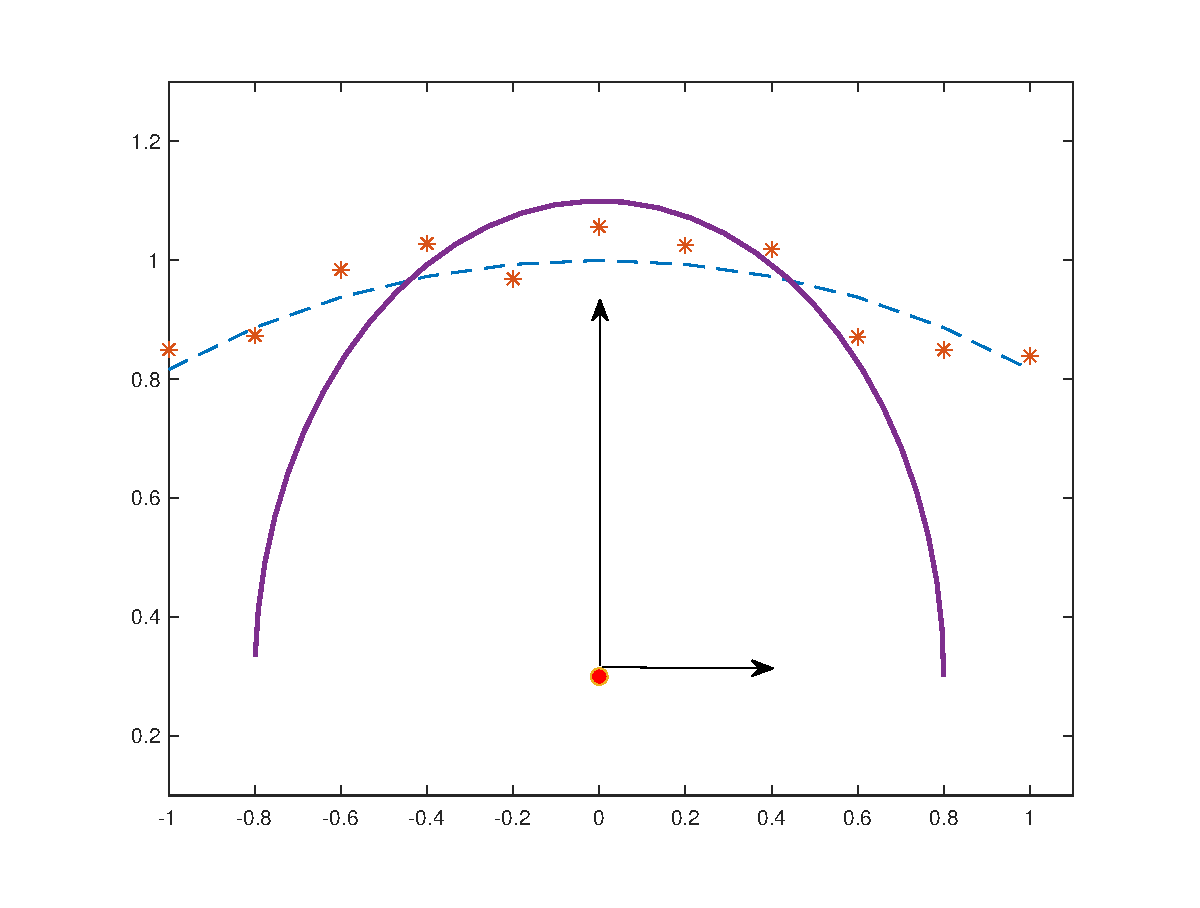
\includegraphics[width=0.32\linewidth]{../figures/demo1.eps} 
\hspace{-4mm}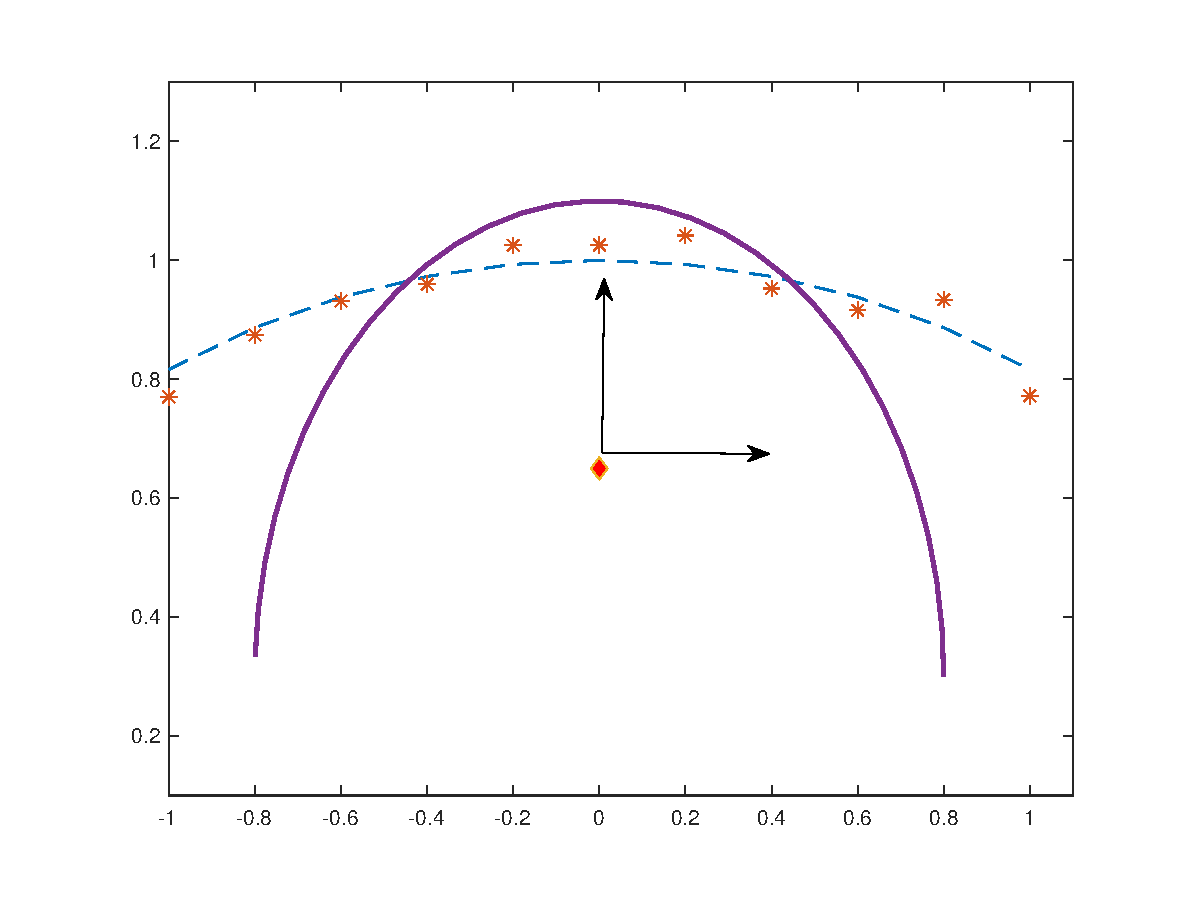
\includegraphics[width=0.32\linewidth]{../figures/demo2.eps} 
\hspace{-4mm}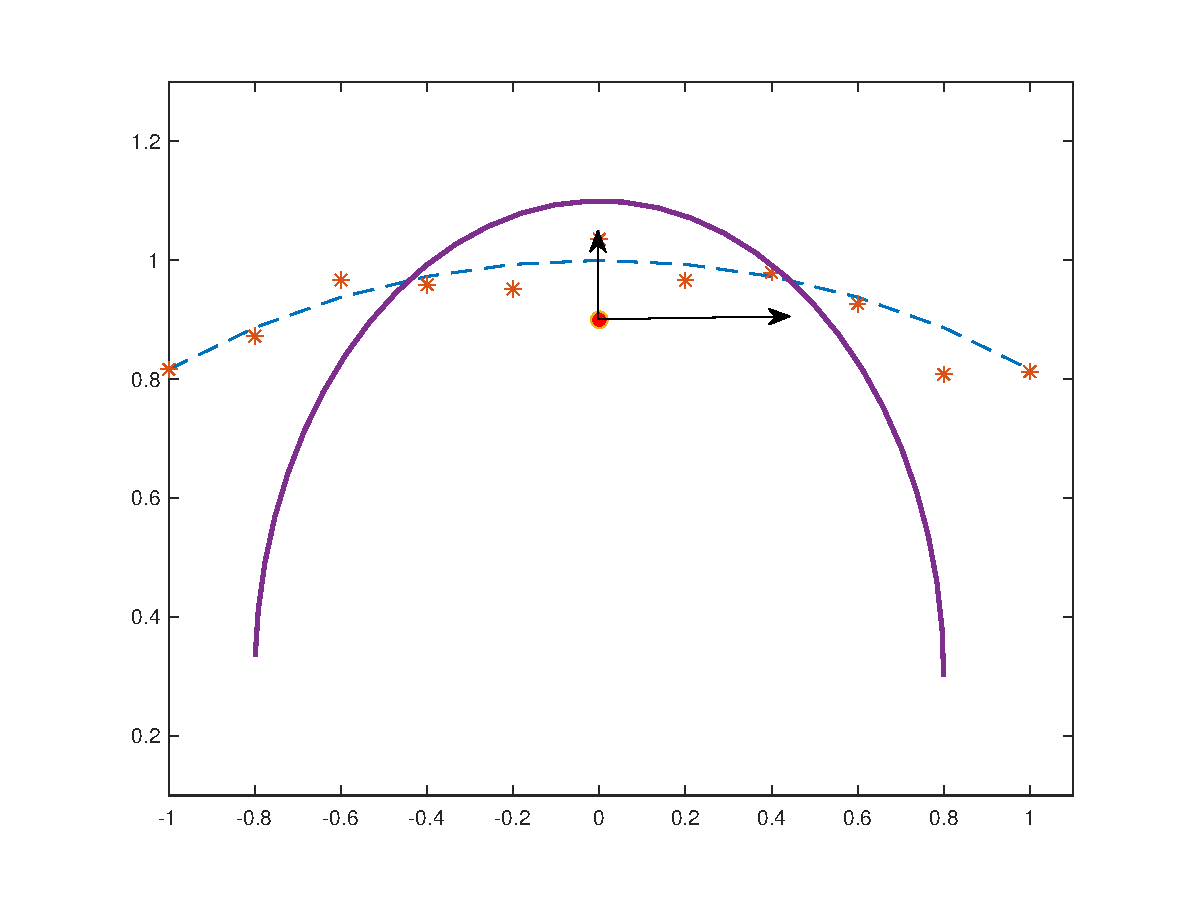
\includegraphics[width=0.32\linewidth]{../figures/demo3.eps} 
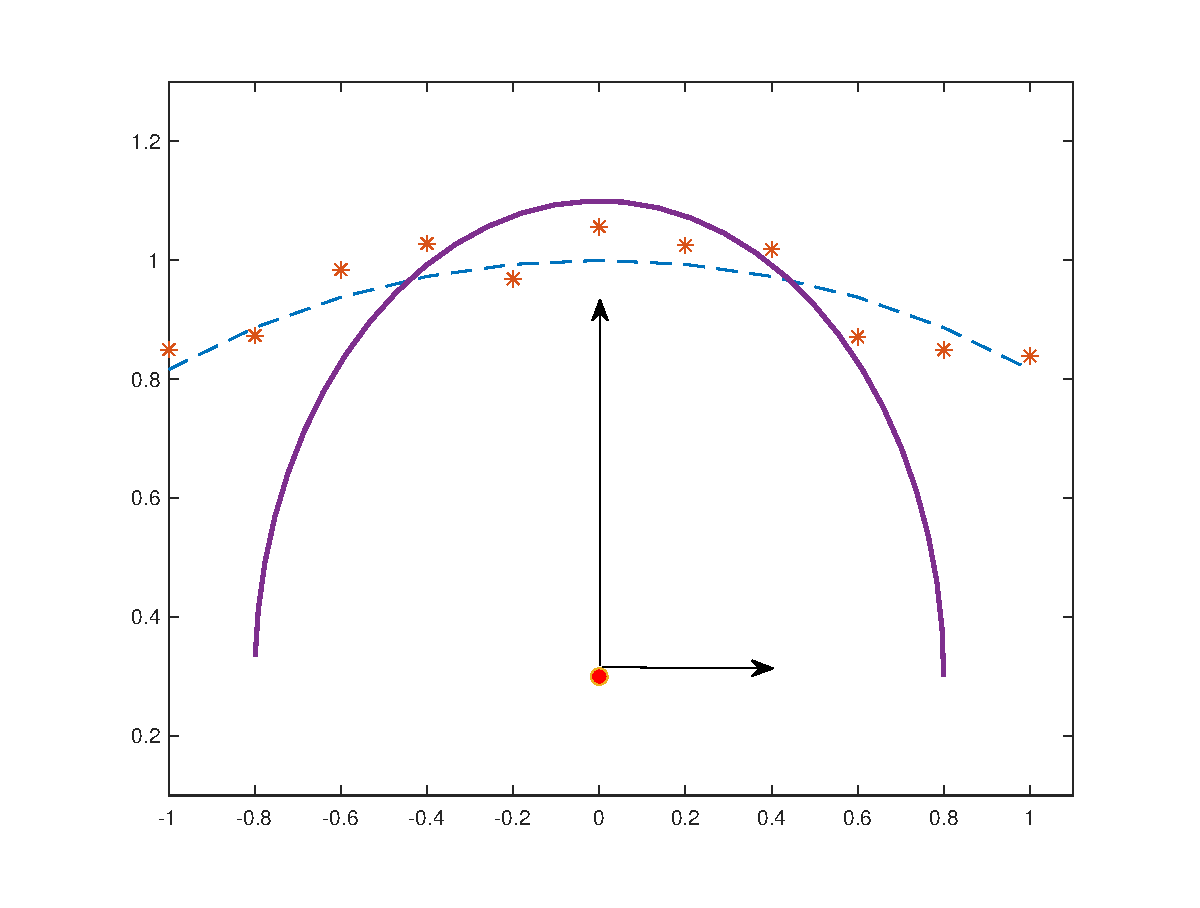
\includegraphics{../figures/demo1.eps}
%\setcaptionwidth{6in}
\caption{The process of $J(x)$'s eigenspace's variation with $x$ approaching the manifold }
\label{Shifting Eigenvectors}
\end{figure}

\begin{figure}
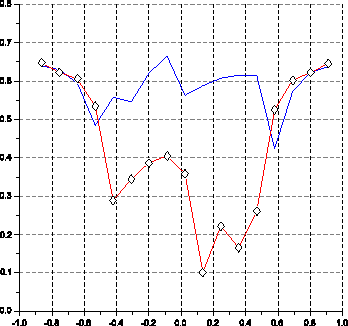
\includegraphics{figure1}
\caption{Pathway of the penicillin G biosynthesis.}
\label{penG}
\end{figure}

Sample of cross-reference to figure.
Figure~\ref{penG} shows that it is not easy to get something on paper.

\section{Equations and the like}

Two equations:
\begin{equation}
    C_{s}  =  K_{M} \frac{\mu/\mu_{x}}{1-\mu/\mu_{x}} \label{ccs}
\end{equation}
and
\begin{equation}
    G = \frac{P_{\mathrm{opt}} - P_{\mathrm{ref}}}{P_{\mathrm{ref}}}  100(\%).
\end{equation}

Equation arrays:
\begin{eqnarray}
  \frac{dS}{dt} & = & - \sigma X + s_{F} F,\\
  \frac{dX}{dt} & = &   \mu    X,\\
  \frac{dP}{dt} & = &   \pi    X - k_{h} P,\\
  \frac{dV}{dt} & = &   F.
\end{eqnarray}
One long equation:
\begin{eqnarray}
 \mu_{\text{normal}} & = & \mu_{x} \frac{C_{s}}{K_{x}C_{x}+C_{s}}  \nonumber\\
                     & = & \mu_{\text{normal}} - Y_{x/s}\bigl(1-H(C_{s})\bigr)(m_{s}+\pi /Y_{p/s})\\
                     & = & \mu_{\text{normal}}/Y_{x/s}+ H(C_{s}) (m_{s}+ \pi /Y_{p/s}).\nonumber
\end{eqnarray}
%%%%%%%%%%%%%%%%%%%%%%%%%%%%%%%%%%%%%%%%%%%%%%
%% Example with single Appendix:            %%
%%%%%%%%%%%%%%%%%%%%%%%%%%%%%%%%%%%%%%%%%%%%%%
\begin{appendix}
\section*{Title}\label{appn} %% if no title is needed, leave empty \section*{}.
Appendices should be provided in \verb|{appendix}| environment,
before Acknowledgements.

If there is only one appendix,
then please refer to it in text as \ldots\ in the \hyperref[appn]{Appendix}.
\end{appendix}
%%%%%%%%%%%%%%%%%%%%%%%%%%%%%%%%%%%%%%%%%%%%%%
%% Example with multiple Appendixes:        %%
%%%%%%%%%%%%%%%%%%%%%%%%%%%%%%%%%%%%%%%%%%%%%%
\begin{appendix}
\section{Title of the first appendix}\label{appA}
If there are more than one appendix, then please refer to it
as \ldots\ in Appendix \ref{appA}, Appendix \ref{appB}, etc.

\section{Title of the second appendix}\label{appB}
\subsection{First subsection of Appendix \protect\ref{appB}}

Use the standard \LaTeX\ commands for headings in \verb|{appendix}|.
Headings and other objects will be numbered automatically.
\begin{equation}
\mathcal{P}=(j_{k,1},j_{k,2},\dots,j_{k,m(k)}). \label{path}
\end{equation}

Sample of cross-reference to the formula (\ref{path}) in Appendix \ref{appB}.
\end{appendix}

%%%%%%%%%%%%%%%%%%%%%%%%%%%%%%%%%%%%%%%%%%%%%%
%% Support information (funding), if any,   %%
%% should be provided in the                %%
%% Acknowledgements section.                %%
%%%%%%%%%%%%%%%%%%%%%%%%%%%%%%%%%%%%%%%%%%%%%%
\section*{Acknowledgements}
The authors would like to thank the anonymous referees, an Associate
Editor and the Editor for their constructive comments that improved the
quality of this paper.

The first author was supported by NSF Grant DMS-??-??????.

The second author was supported in part by NIH Grant ???????????.


%%%%%%%%%%%%%%%%%%%%%%%%%%%%%%%%%%%%%%%%%%%%%%
%% Supplementary Material, if any, should   %%
%% be provided in {supplement} environment  %%
%% with title and short description.        %%
%%%%%%%%%%%%%%%%%%%%%%%%%%%%%%%%%%%%%%%%%%%%%%
\begin{supplement}
\textbf{Title of Supplement A}.
Short description of Supplement A.
\end{supplement}
\begin{supplement}
\textbf{Title of Supplement B}.
Short description of Supplement B.
\end{supplement}

%%%%%%%%%%%%%%%%%%%%%%%%%%%%%%%%%%%%%%%%%%%%%%%%%%%%%%%%%%%%%
%%                  The Bibliography                       %%
%%                                                         %%
%%  imsart-???.bst  will be used to                        %%
%%  create a .BBL file for submission.                     %%
%%                                                         %%
%%  Note that the displayed Bibliography will not          %%
%%  necessarily be rendered by Latex exactly as specified  %%
%%  in the online Instructions for Authors.                %%
%%                                                         %%
%%  MR numbers will be added by VTeX.                      %%
%%                                                         %%
%%  Use \cite{...} to cite references in text.             %%
%%                                                         %%
%%%%%%%%%%%%%%%%%%%%%%%%%%%%%%%%%%%%%%%%%%%%%%%%%%%%%%%%%%%%%

%% if your bibliography is in bibtex format, uncomment commands:
%\bibliographystyle{imsart-number} % Style BST file (imsart-number.bst or imsart-nameyear.bst)
%\bibliography{bibliography}       % Bibliography file (usually '*.bib')

%% or include bibliography directly:
\begin{thebibliography}{4}
%%
\bibitem{r1}
\textsc{Billingsley, P.} (1999). \textit{Convergence of
Probability Measures}, 2nd ed.
Wiley, New York.

\bibitem{r2}
\textsc{Bourbaki, N.}  (1966). \textit{General Topology}  \textbf{1}.
Addison--Wesley, Reading, MA.

\bibitem{r3}
\textsc{Ethier, S. N.} and \textsc{Kurtz, T. G.} (1985).
\textit{Markov Processes: Characterization and Convergence}.
Wiley, New York.

\bibitem{r4}
\textsc{Prokhorov, Yu.} (1956).
Convergence of random processes and limit theorems in probability
theory. \textit{Theory  Probab.  Appl.}
\textbf{1} 157--214.
\end{thebibliography}

\end{document}

